%%%%%%%%%%%%%%%%%%%%%%%%%%%%%%%%%%%%%%%%%
% Masters/Doctoral Thesis 
% LaTeX Template
% Version 2.5 (27/8/17)
%
% This template was downloaded from:
% http://www.LaTeXTemplates.com
%
% Version 2.x major modifications by:
% Vel (vel@latextemplates.com)
%
% This template is based on a template by:
% Steve Gunn (http://users.ecs.soton.ac.uk/srg/softwaretools/document/templates/)
% Sunil Patel (http://www.sunilpatel.co.uk/thesis-template/)
%
% Template license:
% CC BY-NC-SA 3.0 (http://creativecommons.org/licenses/by-nc-sa/3.0/)
%
%%%%%%%%%%%%%%%%%%%%%%%%%%%%%%%%%%%%%%%%%

%----------------------------------------------------------------------------------------
%	PACKAGES AND OTHER DOCUMENT CONFIGURATIONS
%----------------------------------------------------------------------------------------

\documentclass[
12pt, % The default document font size, options: 10pt, 11pt, 12pt
oneside, % Two side (alternating margins) for binding by default, uncomment to switch to one side
english, % ngerman for German
onehalfspacing, % Single line spacing, alternatives: onehalfspacing or doublespacing
%draft, % Uncomment to enable draft mode (no pictures, no links, overfull hboxes indicated)
onehalfspacing, % If the document is onehalfspacing or doublespacing, uncomment this to set spacing in lists to single
%liststotoc, % Uncomment to add the list of figures/tables/etc to the table of contents
%toctotoc, % Uncomment to add the main table of contents to the table of contents
%parskip, % Uncomment to add space between paragraphs
%nohyperref, % Uncomment to not load the hyperref package
headsepline, % Uncomment to get a line under the header
%chapterinoneline, % Uncomment to place the chapter title next to the number on one line
%consistentlayout, % Uncomment to change the layout of the declaration, abstract and acknowledgements pages to match the default layout
]{MastersDoctoralThesis} % The class file specifying the document structure

\usepackage[utf8]{inputenc} % Required for inputting international characters
\usepackage[T1]{fontenc} % Output font encoding for international characters
\usepackage{amsmath}
\usepackage{multirow}
%\usepackage{mathpazo} % Use the Palatino font by default
\usepackage{booktabs}
\usepackage[backend=bibtex,style=numeric-comp,natbib=true,sorting=none]{biblatex} % Use the bibtex backend with the authoryear citation style (which resembles APA)

\addbibresource{example.bib} % The filename of the bibliography

\usepackage[autostyle=true]{csquotes} % Required to generate language-dependent quotes in the bibliography

%----------------------------------------------------------------------------------------
%	MARGIN SETTINGS
%----------------------------------------------------------------------------------------

\geometry{
	paper=a4paper, % Change to letterpaper for US letter
	inner=2.5cm, % Inner margin
	outer=3.8cm, % Outer margin
	bindingoffset=.5cm, % Binding offset
	top=1.5cm, % Top margin
	bottom=1.5cm, % Bottom margin
	%showframe, % Uncomment to show how the type block is set on the page
}

%----------------------------------------------------------------------------------------
%	THESIS INFORMATION
%----------------------------------------------------------------------------------------

\thesistitle{Manifestation of the cluster structure of weakly bound light nuclei in the direct nuclear reactions} % Your thesis title, this is used in the title and abstract, print it elsewhere with \ttitle
\supervisor{Prof. Nunzio \textsc{Itaco}} % Your supervisor's name, this is used in the title page, print it elsewhere with \supname
\examiner{} % Your examiner's name, this is not currently used anywhere in the template, print it elsewhere with \examname
\degree{Doctor of Philosophy} % Your degree name, this is used in the title page and abstract, print it elsewhere with \degreename
\author{Bakytzhan \textsc{Urazbekov}} % Your name, this is used in the title page and abstract, print it elsewhere with \authorname
\addresses{} % Your address, this is not currently used anywhere in the template, print it elsewhere with \addressname

\subject{Theory of nuclear reactions} % Your subject area, this is not currently used anywhere in the template, print it elsewhere with \subjectname
\keywords{} % Keywords for your thesis, this is not currently used anywhere in the template, print it elsewhere with \keywordnames
\university{\href{http://www.unicampania.it}{Luigi Vanvitelli university of Campania}} % Your university's name and URL, this is used in the title page and abstract, print it elsewhere with \univname
\department{\href{http://matfiz.unicampania.it}{Department of Mathematics and Physics}} % Your department's name and URL, this is used in the title page and abstract, print it elsewhere with \deptname
\group{} % Your research group's name and URL, this is used in the title page, print it elsewhere with \groupname
\faculty{} % Your faculty's name and URL, this is used in the title page and abstract, print it elsewhere with \facname

\AtBeginDocument{
\hypersetup{pdftitle=\ttitle} % Set the PDF's title to your title
\hypersetup{pdfauthor=\authorname} % Set the PDF's author to your name
\hypersetup{pdfkeywords=\keywordnames} % Set the PDF's keywords to your keywords
}

\begin{document}
\frontmatter % Use roman page numbering style (i, ii, iii, iv...) for the pre-content pages

\pagestyle{plain} % Default to the plain heading style until the thesis style is called for the body content

%----------------------------------------------------------------------------------------
%	TITLE PAGE
%----------------------------------------------------------------------------------------

\begin{titlepage}
\begin{center}

%\vspace*{.06\textheight}
{\scshape\LARGE \univname\par}\vspace{1.5cm} % University name
\textsc{\Large Doctoral Thesis}\\[0.5cm] % Thesis type

\HRule \\[0.4cm] % Horizontal line
{\huge \bfseries \ttitle\par}\vspace{0.4cm} % Thesis title
\HRule \\[1.5cm] % Horizontal line
 
\begin{minipage}[t]{0.4\textwidth}
\begin{flushleft} \large
\emph{Author:}\\
\href{https://www.researchgate.net/profile/Bakytzhan_Urazbekov}{\authorname} % Author name - remove the \href bracket to remove the link
\end{flushleft}
\end{minipage}
\begin{minipage}[t]{0.4\textwidth}
\begin{flushright} \large
\emph{Supervisor:} \\
\href{https://www.researchgate.net/profile/Nunzio_Itaco}{\supname} % Supervisor name - remove the \href bracket to remove the link  
\emph{Co-Supervisor:} \\
\href{https://www.researchgate.net/profile/A_Denikin}{Prof. Andrey \textsc{Denikin}} %
\end{flushright}
\end{minipage}
\\[3cm] 
%\vfill

%\large \textit{A thesis submitted in fulfillment of the requirements\\ for the degree of \degreename}\\[0.3cm] % University requirement text
%\textit{in the}\\[0.4cm]
%\groupname\\
\deptname
\\[1cm] % Research group name and department name
 
%\vfill

%{\normalsize \today}\\[4cm] % Date
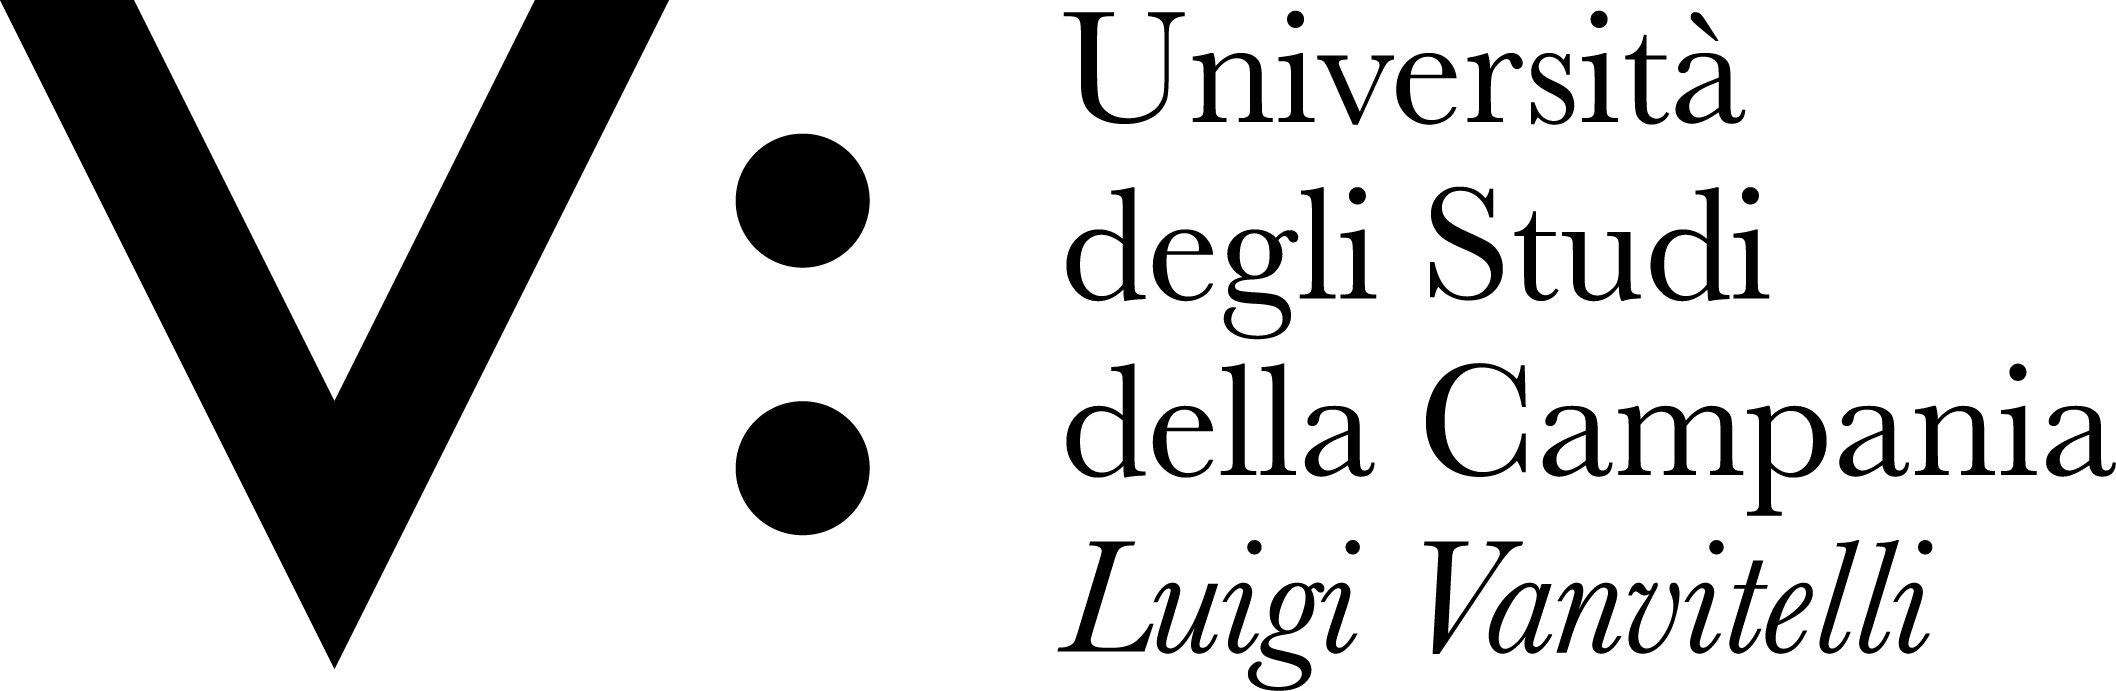
\includegraphics[scale=0.07]{logo} % University/department logo - uncomment to place it
 
%\vfill
\end{center}
\end{titlepage}

%----------------------------------------------------------------------------------------
%	DECLARATION PAGE
%----------------------------------------------------------------------------------------

\begin{declaration}
\addchaptertocentry{\authorshipname} % Add the declaration to the table of contents
\noindent I, \authorname, declare that this thesis titled, \enquote{\ttitle} and the work presented in it are my own. I confirm that:

\begin{itemize} 
\item This work was done wholly or mainly while in candidature for a research degree at this University.
\item Where any part of this thesis has previously been submitted for a degree or any other qualification at this University or any other institution, this has been clearly stated.
\item Where I have consulted the published work of others, this is always clearly attributed.
\item Where I have quoted from the work of others, the source is always given. With the exception of such quotations, this thesis is entirely my own work.
\item I have acknowledged all main sources of help.
\item Where the thesis is based on work done by myself jointly with others, I have made clear exactly what was done by others and what I have contributed myself.\\
\end{itemize}
 
\noindent Signed:\\
\rule[0.5em]{25em}{0.5pt} % This prints a line for the signature
 
\noindent Date:\\
\rule[0.5em]{25em}{0.5pt} % This prints a line to write the date
\end{declaration}

\cleardoublepage

%----------------------------------------------------------------------------------------
%	QUOTATION PAGE
%----------------------------------------------------------------------------------------

\vspace*{0.2\textheight}

\noindent\enquote{\itshape 
By the love of God, the nations are created, and you love them like yourself. Love people as brothers, like freedom, then truth and life are for you. 
}
\bigbreak

\hfill  Abay Qunanbayev

%----------------------------------------------------------------------------------------
%	ABSTRACT PAGE
%----------------------------------------------------------------------------------------

\begin{abstract}
\addchaptertocentry{\abstractname} % Add the abstract to the table of contents

In this work, the following light weakly bound atomic nuclei were studied: $^6$He, $^6$Li and $^9$Be. A three-body model $\alpha$ + 2N for $^6$He and $^6$Li, and 2$\alpha$ + N model for $^9$Be are proposed. The wave function of the three-body system was obtained within the framework of variational calculations based on the Gaussian basis. The interaction potentials for three-body systems have a Pauli projector, which excludes forbidden states. An analytical expression is obtained for the density distribution function of nuclear matter using the three-body wave function. Calculated and given comparisons of root-mean-square matter radii.

The interactions of $^6$He, $^6$Li and $^9$Be have been studied in detail with the simplest particles, such as $\alpha$, $d$, $^3$He. On the basis of the obtained calculations on the density distribution function of nuclear matter, the folding interaction potential was obtained, and shown their comparison with optical potentials with global optical parametrizations. The resulting folding interaction potential is used to calculate the differential cross section for elastic scattering. Using the Coupled Channels approach for $^9$Be the contribution of channels  is studied, and deformation parameters are derived. Comparisons of theoretical cross sections with experimental data in inelastic channels for nuclear reactions $\alpha$ + $^9$Be, $d$ + $^9$Be are given. Within the framework of the Coupled Reaction Channels method, the cross sections for nuclear reactions of single-nucleon and cluster transfers were calculated taking into account the internal structure of atomic nuclei $^6$He, $^6$Li and $^9$Be. Features of the internal structure of these nuclei in direct nuclear reactions are manifested in their mechanism of transfer of clusters and nucleons. In this regard, several mechanisms have been proposed for the transfer of clusters and nucleons in $^6$He, $^6$Li and $^9$Be.

\end{abstract}

%----------------------------------------------------------------------------------------
%	ACKNOWLEDGEMENTS
%----------------------------------------------------------------------------------------

\begin{acknowledgements}
\addchaptertocentry{\acknowledgementname} % Add the acknowledgements to the table of contents
I believe that if it were not for these people, then the thesis in the form in which you are reading, would not have taken place.

I am very grateful to my scientific supervisors Prof. Nunzio Itaco and Prof. Andrey Denikin, who gave a great chance to implement my scientific ideas. Their suggestions, ideas and comments always gave me goals, raised my understanding of science higher and higher.

Undoubtedly, I think it is worthwhile to thank the staff of the Department of Physics and Astronomy and the CIRCE laboratory: Prof. D'Onofrio, Prof. Gialanella, Giuseppe Porzio, Liz, and all members.

In addition, I would like to express my gratitude to Prof. Vladimir Kukulin (Moscow Sate University), who gave advice on a scientific career, Prof Sayabek Sakhiyev (Abay State University), who gave not only scientific guides but also about life.

I also want to thank my dear friends Riccardo Mancino and Felice Pignatelli, without whom I could not just cope with simple life questions in Caserta.

Thanks to Prof. Ian Thompson (LLNL) for explaining the input file for the FRESCO code, Prof. Alexandr Volya (MSU), for providing the values of the spectroscopic amplitudes of alpha particles for p-shell nuclei.

I also dedicate my big thanks to my wife Mervet, who has always supported me at all stages of my scientific career, and my newborn daughter Dina, who has been a source of strength and positiveness.
\end{acknowledgements}

%----------------------------------------------------------------------------------------
%	LIST OF CONTENTS/FIGURES/TABLES PAGES
%----------------------------------------------------------------------------------------

\tableofcontents % Prints the main table of contents

\listoffigures % Prints the list of figures

\listoftables % Prints the list of tables

%----------------------------------------------------------------------------------------
%	ABBREVIATIONS
%----------------------------------------------------------------------------------------

\begin{abbreviations}{ll} % Include a list of abbreviations (a table of two columns)

OM & optical model\\
DF & double folding\\
CC & coupled channel \\
CRC & coupled reaction channels \\
DWBA & distorted wave Born approximation\\
SA & spectroscopic amplitude \\


\end{abbreviations}

%----------------------------------------------------------------------------------------
%	PHYSICAL CONSTANTS/OTHER DEFINITIONS
%----------------------------------------------------------------------------------------

\begin{constants}{lr@{${}={}$}l} % The list of physical constants is a three column table

% The \SI{}{} command is provided by the siunitx package, see its documentation for instructions on how to use it

Speed of Light & $c_{0}$ & \SI{2.99792458e8}{\meter\per\second} (exact)\\
Constant Name & $Symbol$ & $Constant Value$ with units\\

\end{constants}

%----------------------------------------------------------------------------------------
%	SYMBOLS
%----------------------------------------------------------------------------------------

\begin{symbols}{lll} % Include a list of Symbols (a three column table)

%$a$ & distance & \si{\meter} \\
%$P$ & power & \si{\watt} (\si{\joule\per\second}) \\
Symbol & Name & Unit \\

\addlinespace % Gap to separate the Roman symbols from the Greek

$\omega$ & angular frequency & \si{\radian} \\

\end{symbols}

%----------------------------------------------------------------------------------------
%	DEDICATION
%----------------------------------------------------------------------------------------

\dedicatory{to my mom \\~ \\ whom we had immeasurable love of mother and child\ldots} 

%----------------------------------------------------------------------------------------
%	THESIS CONTENT - CHAPTERS
%----------------------------------------------------------------------------------------

\mainmatter % Begin numeric (1,2,3...) page numbering

\pagestyle{thesis} % Return the page headers back to the "thesis" style

% Include the chapters of the thesis as separate files from the Chapters folder
% Uncomment the lines as you write the chapters

\chapter{Introduction} % Main chapter title
In recent years, the study of light weakly bound nuclei  has not lost interest due to the successful development of experimental technology. 
In particular, it should be noted a significant achievement in the field of production of secondary radioactive beams. 
It is known that in light nuclei nucleons tend to group into clusters, the relative motion of which mainly determines the properties and characteristics of the being explored nuclei. 
The cluster structure of the ground and low-lying excited states of light exotic nuclei is one of the priority areas of both experimental and theoretical nuclear physics.


Exotic states in most cases have a rarefied structure and an increased size, which are reflected in rms radii. Such peculiar properties are manifested in the second excited state of the $^{12}$C 7.65 MeV nucleus (Jp = 0+), which in the framework of many well-known models has a cluster structure. 
A similar behavior is predicted for excited states in nuclei 11B and 13C, possibly also having Hoyle states.
 In the framework of the $\alpha$-condensate theory [4, 5], the radius of the Hoyle state is approximately 1.4–1.7 times the radius of the ground state, and the existence of states with a radius close to the radius of uranium nuclei is predicted in $^{12,13}$C and $^{11}$B nuclei.


In the framework of the cluster model, atomic nuclei can be formed from simple particles, such as ions: deuterium-2, tritium-3, hellium-3 alpha and others.
 As an example, $^{6}$He and $^6$Li nuclei can be used. 
 Based on the successful application of theoretical research within the framework of the hyperspherical harmonic model [6], as well as correlation gaussoids [7], it can be deduced that the $^{6}$He and 6Li nuclei are well described by three-body cluster models $\alpha$ + n + n and $\alpha$ + n + p, respectively.
The clustering effect is manifested in many cases in unstable nuclei located on the border of the stability of the nuclear map.
 But there are stable atomic nuclei that clearly show the cluster structure as 7Li, $^{9}$Be, $^{12}$C, and 16O. 
 The $^{9}$Be nucleus is of particular interest for research, since it is a stable, but at the same time weakly bound nucleus. 
 For example, the binding energy of one neutron Sn ($^{9}$Be) = 1.7 MeV in $^{9}$Be is less than the binding energy of one neutron Sn ($^{6}$He) = 1.9 MeV in the unstable $^{6}$He nucleus. 
 Moreover, the $^{9}$Be nucleus has a Borromian structure in which each pair combination in the triple $\alpha$ + $\alpha$ + n structure has no bound state.


The cluster configuration of the $^{9}$Be nucleus is also of interest in nuclear technology. In particular, this nucleus plays an important role in thermonuclear fusion. It is known that the larger the proton number in the atomic nucleus of the wall material, the more the material mixture is formed. In [8] calculations show that with a low proton number the $^{9}$Be nucleus is the most suitable material for the wall of thermonuclear devices. Moreover, if one take into account that the $^{9}$Be nucleus is easily decomposed by electrons and gamma particles into two fast alpha particles, then their kinetic energy contributes to the burning of fuel in the active zone.

It is widely acknowledged that 8Be and 5He nuclei do not exist in nature. 
The lifetime of these nuclei is very short -  approximately 10-20 seconds.
 However, the formation of new elements through these unstable nuclei exists. 
 In particular, the formation of the $^{9}$Be nucleus based on 8Be and 5He nuclei is strongly suppressed. 
 However, in [9] it was shown that under certain circumstances this synthesis is possible. 
% For example, at a temperature of T 109 K, the synthesis of the $^{9}$Be nucleus through the 5Не nucleus becomes dominant.
It is interesting to note the properties of neutron-rich beryllium isotopes. The addition of three neutrons to $^{9}$Be leads to the filling of the neutron p-shell. Along with other beryllium isotopes, the 12Be nucleus has a sufficient lifetime (21.3 ms) for registration and a binding energy of 3.17 MeV greater than the binding energy of the stable beryllium isotope. Therefore, the 12Be core is a remarkable subject of study within the framework of both the shell and cluster models. The study of the structure of radioactive atomic nuclei within the framework of the shell model is interesting because it allows one to take into account all degrees of freedom of nucleons, use realistic effective NN interactions and take into account the contribution of three-nucleon forces when describing the structure of the nucleus [10]. The model describes well the ground states p, sd shell nuclei, but not resonant excitations in the continuous spectrum. To study the state of the continuum, it is necessary to use theoretical approaches that correctly take into account the asymptotic behavior of wave functions at large distances.
Beryllium isotopes exhibit an exceptional $\alpha$-cluster structure — the ground and excited states form molecular structures with two $\alpha$-particles bound by additional neutrons. The configuration of this kind of light nuclei is manifested not only in the structure, but also in the mechanism of interaction with other nuclei. To a large extent, this is observed in the cross sections of the channels of the fusion and transfer reactions. It is also interesting to note that the clustering effect in light nuclei can manifest themselves during the interaction by means of exotic systems, such as 2n, 8Be, 5He, etc. For example, 8Be and 5He nuclei are associated with a breakup as an intermediate channel for a stable $^{9}$Be nucleus. In this case, it is important to note the works [9, 11],  which shows the path of the breakup of this nucleus. In this experimental work, it was proved that low-lying states of the $^{9}$Be nucleus up to an energy of 4 MeV have an n + 8Be configuration, and high-lying excited states from 4 MeV have a 5He + $\alpha$ structure.
In addition to studying the cluster structure in breakup reactions, it is interesting to note the interaction of deuterons with clustered nuclei [12]. In [12] conducted experiments to study the interaction of deuterons with $^{9}$Be nuclei. In particular, the nuclear reaction $^{9}$Be(d,a)7Li should be noted. For this nuclear reaction, different reaction mechanisms were evaluated: direct deuteron transfer, contribution of evaporation residues, and transfer of the 5He heavy cluster. The contribution of the mechanism through the compound nucleus, calculated in the framework of the statistical method, has a small contribution for this reaction at a laboratory energy of 7 MeV. It turned out that a large contribution to the cross section for the (d,a) reaction on the $^{9}$Be nucleus is mainly due to the mechanism of 5He cluster transfer at backward scattering angles. However, [13] concluded that the nuclear reaction $^{9}$Be(d, a)7Li goes through the mechanism the compound nucleus. One of the main arguments in favor of this mechanism is that the energy of the nuclear reaction at 12 and 14 MeV lies precisely in the range of giant resonance in the excitation spectrum of the 11B compound nucleus. In addition, in the work [12], theoretical calculations for the cross section (d, a) of the reaction underestimate the experimental data at the front scattering angles, which suggests the presence of two more direct mechanisms: sequential transfer of the n + p system. Nevertheless, one more experiment should be carried out, and the data should be analyzed in a different energy range. It is assumed that on the basis of a new set of experiments in the framework of the proposed Project, it will be possible to answer the question which mechanism has the greatest contribution to the reaction cross section $^{9}$Be(d,a)7Li.
In Ref. [14 - 16] theoretically studied the reactions of elastic and inelastic scattering, as well as single-nucleon transfers in the interactions of d and 3,4He and with the $^{9}$Be nucleus. The interaction potential of light d and 3,4He particles with $^{9}$Be was calculated in the framework of the folding model using the wave function of the $^{9}$Be ground state in the three-particle 2$\alpha$ + n approximation. Within the framework of the coupled channel method and the distorted wave Born approximaton method, the differential cross sections of inelastic scattering and the reactions of single nucleon transfer were calculated using the folding potential. The obtained angular distributions are in good agreement with experimental data. Thus, it was concluded that the three-cluster approximation $^{9}$Be = 2$\alpha$ + n constructed on the basis of the multicluster dynamic model taking into account the Pauli principle, provides an adequate description of the internal structure and properties of the $^{9}$Be nucleus.  
In particular, interesting information about the properties of exotic nuclei is manifestation of their cluster structure, which can also be obtained from experiments on elastic scattering. The study of exotic states in light nuclei is a priority in the development of nuclear physics in recent decades. Exotic conditions in most cases have a rarefied structure and increased size. Of particular interest is the second excited $^{12}$C state, the Hoyle state, which in many models has a cluster structure and increased dimensions [17, 18]. A similar increase is predicted for states in nuclei 11B and 13C [19, 20], possible analogues of the Hoyle state. As mentioned above, in the framework of the $\alpha$-condensate theory, the radius of the Hoyle state is 1.4–1.7 times the radius of the ground state and the existence of states which has a radius close to the radius of the uranium nucleus are predicted in the $^{12}$C and 11B nuclei.
Hoyle's state plays an important astrophysical role in the synthesis of $^{12}$C in the Universe. The formation of elements heavier than carbon goes through this state. If it would not exist, the rate of carbon formation reaction was 7 orders of magnitude lower. This state is interesting from the hypothesis describing it as a gas of interacting alpha particles, which can be represented as a Bose condensate. Despite numerous studies, the properties of this state, lying above the threshold of decay into three alpha particles, are still poorly understood.
To study the theory of nuclear reactions and its use to describe experimental data a method the Distorted Wave Born Approximation (DWBA) has been successfully applied. The distorted wave method is a good tool for describing nuclear reactions with products registered in the ground state. For transfer channels with excited states, calculations using the DWBA method in many cases give disagreement with the experimental data. In this case, the disagreement is explained by the fact that the wave function of the bound state for the output channel corresponds to a discrete eigenvalue, while the state of this excited nucleus in the experimental data has a resonance with a certain width in the order of several MeV. An adequate theoretical analysis of such problems requires other approaches and methods that require taking into account the degrees of freedom associated with the dynamics of the movement of three clusters and its influence on the mechanisms of nuclear reactions.
The consideration of the continuum in the processes of nuclear reactions is used in the Continuum Discretized Coupled Channels (CDCC) approach [21]. According to the name of the method, the essence of the method consists in discretizing the continuum and in coupling the reaction channels. As in the DWBA method, CDCC requires data which take into account the internal structure of colliding nuclei. The structure is determined by calculations of spectroscopic amplitudes, which strongly depend on the theoretical models under consideration. To date, a well-developed approach for studying the internal structure of the light nuclei of the ground state is ab initio. The ab initio method, which uses realistic NN forces, differs from the shell model in independence from model spaces. There is another method developed on the basis of the CDCC method, this is XCDCC [22]. The addition to the name “X” means taking into account the excited state of the target nucleus. Recently, a continuum discretization method was proposed based on imaginary correlated gaussian functions [23]. This approach successfully describes the displacement phases of elastic scattering of the p +  system and reproduces well the real Coulomb functions.
The aim of this project are: an adequate description of the properties and characteristics of $^{9}$Be and $^{12}$C nuclei using the above methods, obtaining new experimental data on the scattering of light particles by $^{9}$Be and $^{12}$C nuclei, extraction of experimental differential cross sections for elastic, inelastic, single-nucleon and cluster transmission channels. It is expected that the features of the experimental methodology, the latest equipment and modern theoretical approaches will provide an opportunity to better understand the properties and characteristics of the studied nuclei.
Research on this topic is one of the rapidly developing areas of modern nuclear physics of all major scientific centers of the world. Kazakhstan scientists also conduct intensive research in these areas, and work closely with renowned scientists, major research centers, and the results are quite competitive internationally. This is evidenced by the scientific publications of Project managers in international journals with a high impact factor, and thereby show the high importance of this project. New data on the cross sections of nuclear reactions, reliable parameters of the optical potential, and spectroscopic characteristics of the excited states of 5He, 8Be, 10,11,12B, and $^{12}$C nuclei will be useful for testing various cluster nuclear models and for carrying out model calculations of nucleosynthesis reactions for astrophysical and thermonuclear applications.
The project is expected to obtain a number of new and relevant results. The new experimental technique will allow, firstly, to conduct experiments at high energies, and secondly, to experimentally measure cross sections at large scattering angles. In the first case, it is important to note that in the scientific world there are still no enough data on the scattering of 3He and $\alpha$ particles by $^{9}$Be nuclei above energies of 35 MeV. It is very important to conduct an experiment at such energies, since they make it possible to measure the cross sections of relatively heavy reaction products, which reflect direct evidence of cluster transfer. In the second case, modern devices provide a great opportunity to extract information from nuclear reactions at the backward scattering angles. The available information from world-famous databases on the cross section for the 3He + $^{9}$Be reactions for today, unfortunately, has limitations due to poor resolution of detectors. Therefore, the realization of this project, which is not only of academic interest, but also of great practical importance, is highly desirable.

\label{Chapter1} % For referencing the chapter elsewhere, use \ref{Chapter1} 

%----------------------------------------------------------------------------------------

% Define some commands to keep the formatting separated from the content 
\newcommand{\keyword}[1]{\textbf{#1}}
\newcommand{\tabhead}[1]{\textbf{#1}}
\newcommand{\code}[1]{\texttt{#1}}
\newcommand{\file}[1]{\texttt{\bfseries#1}}
\newcommand{\option}[1]{\texttt{\itshape#1}}

%----------------------------------------------------------------------------------------

\chapter{The three body model}
The wave function for the three-body system in the current work was taken from \cite{kukulin1977stochastic}. The work \cite{kukulin1977stochastic} great progress has been made in understanding the structure and properties of the $^6$He, $^6$Li, $^9$Be nuclei based on a three-particle model. It should be noted the progress achieved as a result of the study of the three-body structure, reproduced by the three-body wave function:
\begin{itemize}
\item  structure and static characteristics of the ground state;
\item low-lying excited states and geometric structure;
\item processes of $^6$Li interaction with hadrons, including quasi-elastic scattering ($ \alpha $, 2 $\alpha $), ($ p $, $ d $) and (p, p$\alpha$), high energy proton scattering, and the lightest nuclei on $^6$Li
\item processes of absorption and scattering of $\pi^{\pm}$-mesons by $^6$Li
\item electromagnetic structure;
\item $\beta$-decay of $^6$He and $\mu$-capture by $^6$Li and \textit{etc}.
\end{itemize}

\section{The basis function}
The model \cite{kukulin1977stochastic} uses three pair pseudo-potentials to describe the three-body system, taking into account forbidden states by the Pauli principle:
\begin{equation}
\label{pseudopot}
\widetilde{V}_{ij}=V_{ij}+\Delta_{ij},
\end{equation}
where $V_{ij}$ is  an interaction potential of $(ij)$ subsystem and $\Delta_{ij}=\lambda \Gamma$ is a orthogonalizer with the $\lambda$ constant and with $\Gamma$ projector, which  for  forbidden $f$ state is as follows:
\begin{equation}
\label{projector}
\Gamma=\Gamma(f)=\sum\limits_{m_f}\vert \phi_{fm_f} ({\mathbf x})\rangle \langle  \phi_{fm_f} ({\mathbf x'}) \vert \delta({\mathbf y - \mathbf y'}).
\end{equation}
The principle plays a huge role in the structure of the nucleus, which does not allow overlapping of two constituent particles. Thus, the three body pseudo-Hamiltonian including kinetic energy and pseudo potentials looks like this
\begin{equation}
\label{pseudohamiltonian}
\widetilde{H}=H_0+\sum_{i < j} \widetilde{V }_{ij}.
\end{equation}

As an example, in this work the $2\alpha-n$ three body model of the $^9$Be nucleus is taken. The three-body wave function of the $^9$Be nucleus with total spin $ J $ and spin projection $ M_J $ is represented as
 \begin{equation}
 \Psi^{JM_J}= \sum_{i} C_{i} \psi_{i}^{JM_J} \left( k,pq \right).
 \label{totwf}
 \end{equation}
For simplicity the Jacobi coordinates $ {\bf x}_k $ and $ {\bf y}_k $ are down, the symbols $ k $, $ p $ and $ q $ comply with the cluster indices (see Fig. \ref{fig:jacobiSet}), and the combination of indices ($ k $, $ pq $) corresponds to a certain choice of Jacobi coordinates $ {\bf x}_k $ and $ {\bf y}_k $ of the three-body system, where $ {\bf x}_k $ is a vector of the relative distance between the pair of particles $ pq $ and $ k $, and $ {\bf y}_k $ is the vector of the relative distance between the center of mass of the pair $ pq $ and the particle $ k $. 
The coefficients $ C_{i} $ in Eq.~(\ ref {totwf}) are the parameters of the wave function expansion and are found as a result of solving the generalized eigenvalue problem. 

\begin{figure}[b]
\centering
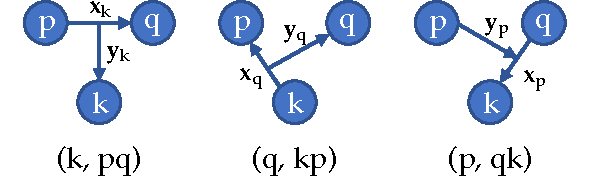
\includegraphics[scale=0.8]{pic1}
\decoRule
\caption{\footnotesize The schemes of Jacobi coordinate sets for the three body system.}
\label{fig:jacobiSet}
\end{figure}

The explicit form of the basis functions $ \psi_{i}^{\gamma} \left(k, pq \right) $ is chosen in the form of the multiplication of the spatial and spin wave functions:
\begin{equation}
\psi_{i}^{JM_J}\left(k, pq \right) = \left[ \phi_{i}^{\gamma} \left(k, pq \right) 
\times \chi^{S} \right] _{JM_{J}},
\label{subwf}
\end{equation}
here the index $\gamma$ includes the quantum numbers $L \lambda l$. The spatial part $\phi_{i}^{\gamma} \left(k, pq \right) $ of the wave function (\ref {subwf}) is constructed using the Gaussian functions:
 \begin{equation}
 \phi_{i}^{\gamma} \left(k, pq \right) =
 x_{k}^{\lambda} y_{k}^{l} exp\left(- \tfrac{1}{2}\alpha^{(k)}_{i} x_{k}^{2} - \tfrac{1}{2} \beta^{(k)}_{i}  y_{k}^{2} \right) 
 \left[ Y_\lambda \left(  \hat{ \bf x}_k \right) \times Y_l \left( \hat{\bf y}_k \right) \right]_{LM_L},
 \label{radial_wf}
 \end{equation}
where $ L $ and $ M_L $ are the total orbital momentum of the system and its projection, $ \lambda $, $ l $ are the orbital moments conjugated to the coordinates $ {\bf x} _k $ and $ {\bf y} _k $ respectively, $ \alpha^{(k)} _ {i} $, $ \beta^{(k)}_{i}$ are the linear parameters of the three-body wave function.
%, the values of which are given in the work \ cite {voronchev1994analysis}.
 \section{Transformation of the basis function }
 The chosen form of the basis function (\ref{subwf}) is convenient in that it can be easily transformed for use with an alternative set of Jacobi coordinates. A rotation matrix connecting different sets of the Jacobi coordinates is provided through
 
\begin{equation}
\begin{pmatrix}
{\bf x}_k \\ 
{\bf y}_k
\end{pmatrix}  = {\bf T}^{(kq)}
\begin{pmatrix}
{\bf x}_q \\ 
{\bf y}_q
\end{pmatrix}.
\end{equation}
here, particularly for  the $(kq)$ transition, the ${\bf T}^{(kq)}$ matrix is 
\begin{equation}
{\bf T}^{(kp)} = 
 \begin{pmatrix}
 {\bf T}^{(kq)}_{11} & {\bf T}^{(kq)}_{12} \\
 {\bf T}^{(kq)}_{21}  &  {\bf T}^{(kq)}_{22}
 \end{pmatrix}
=
 \begin{pmatrix}
 -\tfrac{m_p}{m_p+m_q} & 1 \\
 -\tfrac{m_q(m_k+m_p+m_q)}{(m_p+m_q)(m_k+m_q)}  &  -\tfrac{m_k}{(m_k+m_q)}.
 \end{pmatrix}
\end{equation}

There is no need to consider the transformation of spin part of the basis function. The reason is that the $S$ spin of the $2\alpha-n$ three-body system is defined only by the vacant nucleon, and it doesn't depend on the choice of the Jacobi coordinate. That is to say, the coupling of the vacant nucleon spin with the $\alpha-\alpha$ subsystem spin gives again the spin of the nucleon due to the $\alpha$ particles having a spin of zero.  

The transformation of the space part of the wave function from the set $ \left(k, qp \right) $ to the set $ \left(q, kp \right) $ can be expressed in the following way

  \begin{equation}
 \label{transformbasisfunction}
 \phi_{i}^{\gamma}\left(k, pq \right) = \sum_{\tilde{\gamma}} A_{\tilde{\gamma}\gamma}\left( {\bf T}^{(kq)} \right)
  \phi_{i}^{\tilde{\gamma} } \left(q, kp \right) ,
 \end{equation}
where the sum is over quantum numbers of the $ \tilde {\gamma} $ new set, and the new basis function is
\begin{align}
\phi_{i}^{\tilde{\gamma} } \left(q, kp \right)  =  &
 x_{q}^{\tilde{\lambda}} y_{q}^{\tilde{l}} exp\left(- \tfrac{1}{2} \alpha^{(q)}_{i} x_{q}^{2} - \tfrac{1}{2} \beta^{(q)}_{i}  y_{q}^{2} - \rho^{(q)}_i {\bf x}_{q} \cdot {\bf y}_{q}  \right) 
\times  \nonumber \\ 
&\times  \left[ Y_{\tilde{\lambda}} \left(  \hat{ \bf x}_q \right) \times Y_{\tilde{l}} \left( \hat{\bf y}_q \right) \right]_{LM_L},
\label{newBasis}
\end{align}
%, !taking into account the condition $ \tilde{\lambda} + \tilde{l} = \lambda + l $!.
where new parameters of the wave function are given by
\begin{align}
\begin{pmatrix}
\alpha_i^{(q)} & \rho_i^{(q)} \\ 
\rho_i^{(q)} & \beta_i^{(q)}
\end{pmatrix}  = \left( {\bf T}^{(kq)} \right)^{T} \times 
\begin{pmatrix}
\alpha_i^{(k)} & \rho_i^{(k)} \\ 
\rho_i^{(k)} & \beta_i^{(k)}
\end{pmatrix} \times  {\bf T}^{(kq)}.
\end{align}
%\nonumber \\
%\alpha^{(q)}_{i} =& \alpha^{(k)}_{i} T_{11}^2 + \beta^{(k)}_{i} T_{21}^2 
%\nonumber \\
%\beta^{(q)}_{i} =& \alpha^{(k)}_{i} T_{12}^2 + \beta^{(k)}_{i} T_{22}^2 
%\nonumber \\
%\rho^{(q)}_{i} =& 2 \alpha^{(k)}_{i} T_{11} T_{12} + 2 \beta^{(k)}_{i} T_{21}  T_{22} 
Note, that for the $(k,pq)$ coordinate set the radial wave function (\ref{radial_wf}) does not include the scalar product ${\bf x}_k \cdot {\bf y}_k$, which means $\rho_i^{(k)}=0$.  
 Using Eq.~(\ref{sphHarmDecomp}) and~(\ref{hyperSphTrans}) it is easy to get the coupling coefficient $ A_{\tilde{\gamma} \gamma} \left( {\bf T}^{(kq)} \right) $ from Eq.~(\ref{transformbasisfunction}), which is defined as follow 
 \begin{align}
A_{\tilde{\gamma}\gamma}\left( {\bf T}^{(kq)} \right) = & \sum_{\lambda_1 \lambda_2 l_1 l_2} 
\left({\bf T}_{11}^{(kq)} \right)^{\lambda_1} 
\left({\bf T}_{12}^{(kq)} \right)^{\lambda_2} 
\left({\bf T}_{21}^{(kq)} \right)^{l_1} 
\left({\bf T}_{22}^{(kq)} \right)^{l_2} 
\times \nonumber
\\
& \times {E}^{\lambda_1 \lambda_2 \lambda l_1 l_2 l L}_{\tilde{\lambda} \tilde{l} } \mathcal{D}(\lambda,\lambda_1,\lambda_2) \mathcal{D}(l,l_1,l_2).    
\label{trans_coef}
\end{align}

\section{Overlap matrix elements}
Within the $\left(k, pq \right)$ scheme an overlap matrix element, in particular for the space part $ \phi_{i}^{\gamma}\left(k, pq \right)$ of the basis function, is expressed by
\begin{equation}
\langle \phi_{i}^{\gamma}\left(k, pq \right) \vert 
\phi_{j}^{\gamma^{\prime}}\left(k, pq \right) \rangle= \int \int d{\bf x}_k d{\bf y}_k ~\phi_{i}^{\gamma}\left(k, pq \right) \left( \phi_{j}^{\gamma^{\prime}}\left(k, pq \right) \right)^{*}.
\end{equation}
Following the properties of spherical harmonics the latter six dimensional integral gets $\delta_{\gamma \gamma^{\prime}}$. Then, it  is reduced to analytical expression as  
\begin{equation}
\mathcal{I} \left( \lambda,l,\alpha_{ij}^{(k)},\beta_{ij}^{(k)} \right)= 2^{1+\lambda+l}\frac{\Gamma \left( \frac{3}{2}+\lambda \right) \Gamma \left( \frac{3}{2}+l \right) }{ \left( \alpha_{ij}^{(k)} \right) ^{\frac{3}{2}+\lambda} \left( \beta_{ij}^{(k)} \right) ^{\frac{3}{2}+l}} .
\end{equation}
with 
\begin{equation}
\alpha_{ij}^{(k)}=\alpha_{i}^{(k)}+\alpha_{j}^{(k)}~~~~~~
\beta_{ij}^{(k)}=\beta_{i}^{(k)}+\beta_{j}^{(k)}
\end{equation}


However, to calculate overlap matrix elements for arbitrary basis functions, for example
\begin{equation}
\langle \phi_{i}^{\tilde{\gamma}}\left(q,kp \right) \vert 
\phi_{j}^{\tilde{\gamma}^{\prime}}\left(q,kp \right) \rangle =
\int \int d{\bf x}_k d{\bf y}_k ~\phi_{i}^{\tilde{\gamma}}\left(q,kp \right) \left( \phi_{j}^{\tilde{\gamma}^{\prime}}\left(q,kp \right) \right)^{*},
\label{me_arb}
\end{equation}
one must handle with the scalar product $exp\left(- \rho {\bf x} \cdot {\bf y} \right)$ in  Eq.~(\ref{newBasis}), in which radial and angular parts are mixed. It makes a problem in integration procedure, consequently, mathematical techniques must be applied. There are two tricks to solve this problem.  First is the solution of problem is in expansion of  the exponential function into the partial waves. Another one is in projection of the factor of scalar product into the rotation matrix ${\bf T}$. Both approaches give the same results in calculation of the matrix elements. 
\subsection{By means of the  exponential function expansion}
\label{overlap_by_exp}
The expansion of exponential function is given by 
\begin{equation}
exp(-\rho {\bf x} \cdot {\bf y}) = 4 \pi \sum_{\kappa} \sqrt{2\kappa+1} 
\epsilon(\kappa, \rho)i_{\kappa}(|\rho|xy)Y_{00}^{(\kappa\kappa)}(\hat{{\bf x}},\hat{{\bf y}})
\end{equation} 
where $i_{\kappa}(x) $ -- modified spherical Bessel function of the first kind, $\epsilon(\kappa, \rho)=(-1)^{\kappa}$ for $\rho \le 0$, otherwise it equals to $1$.
Once radial part is separated, defining an integral
\begin{equation}
\int_0^\infty \int_0^\infty  dx dy~ x^{2\lambda+\kappa+2}y^{2 l +\kappa+2} exp\left( -\alpha x^2 - \beta y^2 \right) i_{\kappa}(|\rho|xy),
\end{equation}
one can get its analytical form
\begin{align}
\mathcal{I}(\lambda, l, n, \alpha, \beta, |\rho|) =& \sqrt{\frac{\pi}{8}}(2l)!!~ \Gamma(l+n+\tfrac{3}{2})~|\rho|^{n} ~\beta^{-l-n-\tfrac{3}{2}} \times \nonumber \\
& \times \sum_{\kappa=0}^{l} \frac{\Gamma(\kappa+\lambda+n+\tfrac{3}{2})}{\kappa! (l-\kappa)! \Gamma(\kappa+n+\tfrac{3}{2})}
\left(\frac{\rho^2}{2\beta}\right)^{\kappa} \left( \frac{\alpha}{2} - \frac{\rho^2}{2\beta}  \right)^{-\kappa-\lambda-n-\tfrac{3}{2}}.
\label{overlap1}
\end{align}
The angular part is integrated all over angular variables, then,  it can be expressed analytically in the following way
\begin{align}
\int \int d\hat{\bf x}~d\hat{\bf y}~ Y_{00}^{(\kappa\kappa)}(\hat{{\bf x}},\hat{{\bf y}})  Y_{L^{\prime}M_{L^{\prime}}}^{(\lambda^{\prime} l^{\prime})}(\hat{{\bf x}},\hat{{\bf y}}) \left(  Y_{LM_L}^{(\lambda l)}(\hat{{\bf x}},\hat{{\bf y}}) \right)^{*} =  {E}^{\kappa \kappa 0 \lambda^{\prime} l^{\prime} L L}_{\lambda l} \delta_{LL^{\prime}} 
\label{angular_part_overlap1}
\end{align}

Using the property of the 9-j symbol, in which one of the numbers is zero, ${E}^{\kappa \kappa 0 \lambda^{\prime} l^{\prime} L L}_{\lambda l}$ can be reduced as
\begin{equation}
{E}^{\kappa \kappa 0 \lambda^{\prime} l^{\prime} L L}_{\lambda l}
=U\left(  \lambda L \kappa l^{\prime};~ l \lambda^{\prime} \right) \frac{\mathcal{C} \left( \lambda^{\prime}, \lambda, \kappa \right) \mathcal{C} \left( l^{\prime}, l, \kappa \right) }{ \sqrt{\left( 2L+1 \right) \left( 2\kappa +1 \right)}}.
\end{equation}

The Jacobian  matrix ${\bf J}^{(kq)}$ for transformation from the ${\bf x}_k, {\bf y}_k$ coordinates to the ${\bf x}_q, {\bf y}_q$ coordinates gives the ${\bf T}^{(kq)}$ matrix
\begin{equation}
{\bf J}^{(kq)} = 
\begin{pmatrix}
\frac{\partial {\bf x}_k \left({\bf x}_q,{\bf y}_q \right)}{ \partial {\bf x}_q }  
& \frac{\partial {\bf x}_k \left({\bf x}_q,{\bf y}_q \right)}{ \partial {\bf y}_q } \\
\frac{\partial {\bf y}_k \left({\bf x}_q,{\bf y}_q \right)}{ \partial {\bf x}_q }  
& \frac{\partial {\bf y}_k \left({\bf x}_q,{\bf y}_q \right)}{ \partial {\bf y}_q } 
\end{pmatrix} = {\bf T}^{(kq)}.
\end{equation}
Accordingly, the determinant $\vert {\bf J}^{(kq)} \vert$ is a determinant of the ${\bf T}^{(kq)}$ matrix, which equals to $1$:
\begin{equation}
\vert {\bf J}^{(kq)} \vert = \vert {\bf T}^{(kq)} \vert =1
\end{equation}
  Therefore, the integration variables in Eq.~(\ref{me_arb}) can be changed without any factorization. 
  
  Lastly, an expression for the overlap matrix element of the $(q,kp)$ coordinate sets ~(\ref{me_arb}) can be determined as follow
\begin{align}
\langle \phi_{i}^{\tilde{\gamma}}\left(q,kp \right) & \vert 
\phi_{j}^{\tilde{\gamma}^{\prime}}\left(q,kp \right) \rangle =
\int \int d{\bf x}_k d{\bf y}_k  ~\phi_{i}^{\tilde{\gamma}}\left(q,kp \right) \left( \phi_{j}^{\tilde{\gamma}^{\prime}}\left(q,kp \right) \right)^{*}  = \nonumber 
\\ & = 4 \pi \sum_{\tilde{\gamma}\tilde{\gamma}^{\prime}}  A_{\gamma\tilde{\gamma}}\left( T^{(kq)} \right) A_{\gamma\tilde{\gamma}^{\prime}}\left( T^{(kq)} \right)
 \sum_{\kappa} \sqrt{2\kappa+1}~ \epsilon(\kappa, \rho) {E}^{\kappa \kappa 0 \lambda^{\prime} l^{\prime} L L}_{\lambda l} \times  \nonumber \\
 &\times \mathcal{I}\left(
 \tfrac{\tilde{\lambda}+\tilde{\lambda^{\prime}}-\kappa}{2}, ~
 \tfrac{\tilde{l}+\tilde{l^{\prime}}-\kappa}{2},~
 \kappa,~
 \alpha^{(q)}_{ij},~
 \beta^{(q)}_{ij} ,~
 \vert \rho^{(q)}_{ij} \vert ~
  \right).
\end{align}
with $\rho_{ij}^{(q)}=\rho_{i}^{(q)}+\rho_{j}^{(q)}$.

\subsection{By means of the projection into the ${\bf T}$ matrix}
\label{overlap_by_proj}
In this approach the rotation matrix ${\bf Q}$, projecting the scalar product in the radial part of the wave function, is implemented by
\begin{equation}
{\bf Q}_i^{(kq)}= {\bf T}^{(kq)} \times
\begin{pmatrix}
1 & -\tfrac{\rho^{(q)}_{i}}{\alpha^{(q)}_i} \\ 
0 & 1
\end{pmatrix} .
\end{equation}
Consequently, the radial part of the wave function can be rewritten with no scalar product term as
\begin{align}
\phi_{i}^{\tilde{\gamma} } \left(q, kp \right)  =  &
 x_{q}^{\tilde{\lambda}} y_{q}^{\tilde{l}} exp\left(- \tfrac{1}{2} \alpha^{(q)}_{i} x_{q}^{2} - \tfrac{1}{2} \left(  \beta^{(q)}_{i} - \tfrac{\left(\rho^{(q)}_i\right)^2}{\alpha^{(q)}_i} \right)  y_{q}^{2}  \right) 
\times  \nonumber \\ 
&\times  \left[ Y_{\tilde{\lambda}} \left(  \hat{ \bf x}_q \right) \times Y_{\tilde{l}} \left( \hat{\bf y}_q \right) \right]_{LM_L}.
\end{align}
One can get easily the expression of the overlap matrix element for the $(q,kp)$ coordinate sets ~(\ref{me_arb}) can be determined as follow
\begin{align}
\langle \phi_{i}^{\tilde{\gamma}}\left(q,kp \right) & \vert 
\phi_{j}^{\tilde{\gamma}^{\prime}}\left(q,kp \right) \rangle =
\int \int d{\bf x}_k d{\bf y}_k  ~\phi_{i}^{\tilde{\gamma}}\left(q,kp \right) \left( \phi_{j}^{\tilde{\gamma}^{\prime}}\left(q,kp \right) \right)^{*} =  \nonumber \\
=& \sum_{\tilde{\gamma}\tilde{\gamma}^{\prime}}  
A_{\gamma\tilde{\gamma}}\left( {\bf Q}_{ij}^{(kq)} \right)
 A_{\gamma\tilde{\gamma}^{\prime}}\left( {\bf Q}_{ij}^{(kq)} \right) \mathcal{I} \left( \tilde{\lambda}, \tilde{l}, \alpha^{(q)}_{ij}, \left(  \beta^{(q)}_{ij} - \tfrac{\left(\rho^{(q)}_{ij}\right)^2}{\alpha^{(q)}_{ij}} \right) \right) \delta_{\tilde{\gamma}\tilde{\gamma}^{\prime}}.
 \label{projectionMethod}
\end{align}
Analogously, changing the integration variables is carried out with no factorizations due to the $\vert {\bf Q}_i^{(kq)} \vert = 1$. Notably,   rotation matrix becomes depended on the $ij$ indexes in this approach.


\section{Normalization and correlation density of the three-body wave function}
Using the overlap matrix elements the normalization of the total three-body wave function is given by
\begin{align}
\mathcal{N}^{(k)}= & \langle \Psi^{JM_J} \vert \Psi^{JM_J} \rangle = \sum_{\gamma} \mathcal{N}^{(k)}_{\gamma},    \nonumber \\
 \mathcal{N}^{(k)}_{\gamma} = & \sum_{ij} C_i C_j \mathcal{I} \left( \lambda,l,\alpha_{ij}^{(k)},\beta_{ij}^{(k)} \right).
\end{align}
For the alternative set of Jacobi coordinates the overlap of the total wave function is given by
\begin{equation}
\mathcal{N}^{(q)}= \langle \Psi^{JM_J} \vert \Psi^{JM_J} \rangle = \sum_{\gamma} \sum_{\gamma^{\prime}} \mathcal{N}^{(q)}_{\gamma \gamma^{\prime}}
\end{equation}
It should be mentioned, that in the latter expression the basis functions is not orthogonal. Therefore, according to the Eq.~(\ref{angular_part_overlap1}) the sum is limited with the condition $\delta_{LL^{\prime}}$ only. Using the analytical form  of overlap matrix element (\ref{overlap1}), $\mathcal{N}^{(q)}_{\gamma \gamma^{\prime}}$ can be given by
\begin{align}
\mathcal{N}^{(q)}_{\gamma \gamma^{\prime}}= & 4 \pi \sum_{ij} C_i C_j \sum_{\tilde{\gamma}\tilde{\gamma}^{\prime}}  A_{\gamma\tilde{\gamma}}\left( {\bf T}^{(kq)} \right) A_{\gamma\tilde{\gamma}^{\prime}}\left( {\bf T}^{(kq)} \right) \times
\nonumber \\
 & \times \sum_{\kappa} \sqrt{2\kappa+1}~ \epsilon(\kappa, \rho^{(k)}_{ij}) {E}^{\kappa \kappa 0 \lambda^{\prime} l^{\prime} L L}_{\lambda l} \times  \nonumber 
 \\ & \times \mathcal{I}\left(
 \tfrac{\tilde{\lambda}+\tilde{\lambda^{\prime}}-\kappa}{2}, ~
 \tfrac{\tilde{l}+\tilde{l^{\prime}}-\kappa}{2},~
 \kappa,~
 \alpha^{(q)}_{ij},~
 \beta^{(q)}_{ij} ,~
 \vert \rho^{(q)}_{ij} \vert ~
  \right),
\end{align}
or using the Eq.~(\ref{projectionMethod})
\begin{align}
\mathcal{N}^{(q)}_{\gamma \gamma^{\prime}}= & \sum_{ij} C_i C_j  \sum_{\tilde{\gamma}\tilde{\gamma}^{\prime}}
A_{\gamma\tilde{\gamma}}\left( {\bf Q}_{ij}^{(kq)} \right)
 A_{\gamma\tilde{\gamma}^{\prime}}\left( {\bf Q}_{ij}^{(kq)} \right) \times\nonumber \\
 & \times
  \mathcal{I} \left( \tilde{\lambda}, \tilde{l}, \alpha^{(q)}_{ij}, \left(  \beta^{(q)}_{ij} - \tfrac{\left(\rho^{(q)}_{ij}\right)^2}{\alpha^{(q)}_{ij}} \right) \right) \delta_{\tilde{\gamma}\tilde{\gamma}^{\prime}}.
\end{align}  

A correlation density function of the total wave function (\ref{totwf})  can be expressed in the following way
\begin{align}
W\left( x_k,y_k \right) =& \sum_{\gamma} W_{\gamma}\left( x_k,y_k \right) \nonumber \\
W_{\gamma}\left( x_k,y_k \right) =& \sum_{ij} C_i C_j x^{2+2\lambda}_k y^{2+2l}_k \text{exp}\left( - \tfrac{1}{2} \alpha^{(k)}_{ij} x_k^2 -  \tfrac{1}{2} \beta^{(k)}_{ij} y_k^2 \right) .
\end{align}
 
% Please add the following required packages to your document preamble:
% \usepackage{booktabs}
\begin{table}[bp]
\footnotesize
\begin{tabular}{@{}ccccc@{}}
\toprule
                                    & \multicolumn{4}{c}{$\gamma \equiv \lambda l L$} \\
                                    & 011     & 211     & 212     & 231               \\ \midrule
$\mathcal{N}_{\gamma}^{(k)}$        & 0.4358  & 0.3619  & 0.1826  & 0.0091            \\
$\mathcal{N}_{\gamma \gamma}^{(q)}$ & 0.4358  & 0.3619  & 0.1826  & 0.0091            \\
$W_{\gamma}\left(x_k,y_k\right)$    
&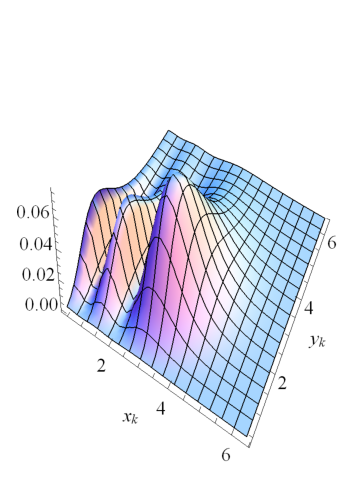
\includegraphics[scale=0.5]{W1_1}         
&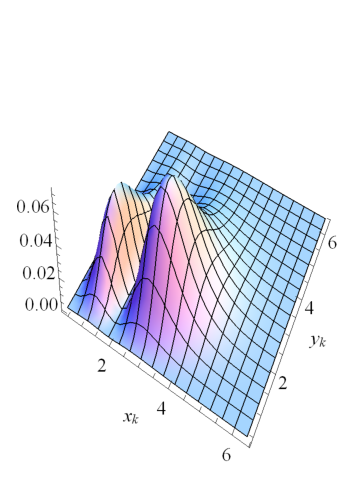
\includegraphics[scale=0.5]{W1_2}         
&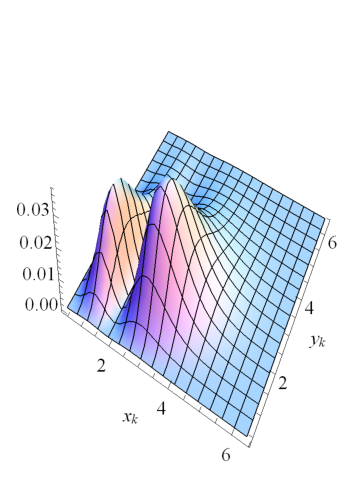
\includegraphics[scale=0.5]{W1_3}         
&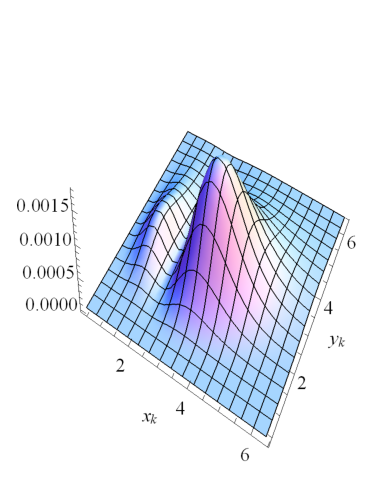
\includegraphics[scale=0.5]{W1_4}                   
\\ \midrule
                                    & \multicolumn{4}{c}{$\gamma \equiv \lambda l L$} \\ 
                                    & 232     & 431     & 432     & $\sum_i \gamma_i$ \\ \midrule
$\mathcal{N}_{\gamma}^{(k)}$        & 0.0022  & 0.0064  & 0.0019  & 1.0               \\
$\mathcal{N}_{\gamma \gamma}^{(q)}$ & 0.0022  & 0.0064  & 0.0019  & 1.0               \\
$W_{\gamma}\left(x_k,y_k\right)$    
&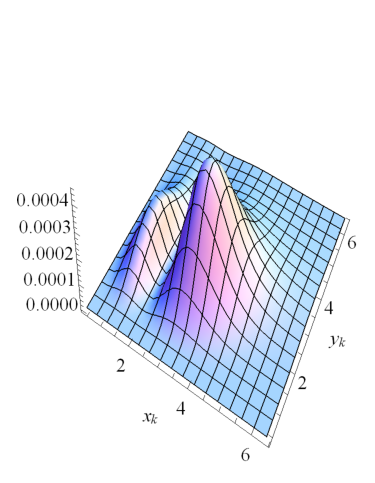
\includegraphics[scale=0.5]{W1_5}         
&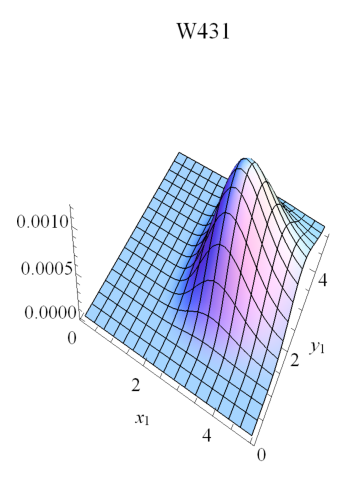
\includegraphics[scale=0.5]{W1_6}         
&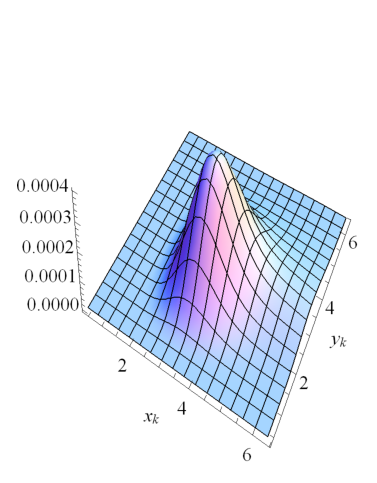
\includegraphics[scale=0.5]{W1_7}         
&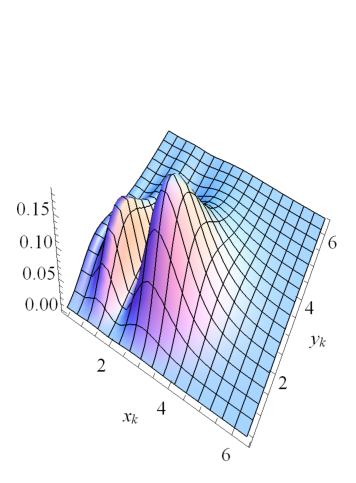
\includegraphics[scale=0.5]{W1_all}                  
\\ \bottomrule
\end{tabular}
\caption{
\footnotesize
Values of the $\mathcal{N}_{\gamma}^{(k)}$ and  $\mathcal{N}_{\gamma \gamma}^{(q)}$ normalizations for each $\gamma$'s, and 3-d plot of the correlation density function $W_{\gamma}\left(x_k,y_k\right)$ of the wave function depending on $\gamma$.}
\label{table:atable}
\end{table}


\section{The density distribution function of nuclear matter}

An operator of matter density distribution of the three body system takes the sums of all three clusters and brings it from the center of  system mass 
\begin{equation}
\rho(\textbf{R})=\sum_{\scriptscriptstyle{cluster}=i,j,k} \rho_{\scriptscriptstyle cluster}(\textbf{R}) .
\end{equation}
In particular,  nucleon cluster is treated as point like particle, while in alpha cluster  one takes into account its internal structure  (see Fig.2)  $ \displaystyle \rho_\alpha(r_{\alpha})=\rho_0 \exp\left(-\gamma_0 r^2_{\alpha} \right)$ with parameters $ \displaystyle \gamma_0= 0.7024$, $  \displaystyle \rho_0=0.4229$ \cite{satchler1979folding}. So corresponding matrix elements for both nucleon cluster and alpha cluster are
\begin{equation}
\label{densities}
\begin{gathered}
\rho_{N_i}(\textbf{R})=
\langle\varphi^{{\gamma}}(i,jk) 
\vert \delta(\textbf{R}-\textbf{y}_i)
\vert \varphi^{{\gamma}}(i,jk)\rangle \\
\rho_{\alpha_i}(\textbf{R})= 
\langle\varphi^{{\gamma}}(i,jk) 
\vert \rho_{\alpha}(\textbf{R}-\textbf{y}_i) \delta(\textbf{y}_i-\textbf{r}_\alpha)
\vert \varphi^{{\gamma}}(i,jk)\rangle \\
\end{gathered}
\end{equation}


In the case of the cluster is in another set of coordinate, one can express taking the equation \eqref{basisfunction}
\begin{align*}
\begin{gathered}
\rho_{N_j}(\textbf{R})=
\sum_{  \widetilde{ \gamma }     } A_{\Omega}^{j \leftarrow i}  A_{\Omega}^{j \leftarrow i} 
\langle \varphi^{ \widetilde{\gamma} }(j,ki) 
\vert \delta(\textbf{R}-\textbf{y}_j)
\vert \varphi^{\widetilde{\gamma}}(j,ki)\rangle \\
\rho_{\alpha_j}(\textbf{R})= 
\sum_{  \widetilde{ \gamma }     } A_{\Omega}^{j \leftarrow i}  A_{\Omega}^{j \leftarrow i} 
\langle \varphi^{ \widetilde{\gamma} }(j,ki) 
\vert \rho_{\alpha}(\textbf{R}-\textbf{y}_j) \delta(\textbf{y}_j-\textbf{r}_{\alpha})
\vert \varphi^{\widetilde{\gamma}}(j,ki)\rangle.\\
\end{gathered}
\end{align*}




 Using the well known expansion of exponent function
\begin{align*}
\exp(-\rho_0 \textbf{R} \cdot \textbf{y} )=
4 \pi \sum_k \sqrt{2k+1} \text{ } i_k(\rho_0 R y) Y^{kk}_{00} \left( \widehat{R},\widehat{y} \right)
\end{align*}
and an analytical expression of integral kind of
\begin{align*}
\int_0^\infty y^{2l+k+2}\exp(-\beta y^2)i_k(\mu y) dy=
\sqrt{\frac{\pi}{2}} \frac{   (2l)!!   (\mu)^k}{   \left( \frac{1}{2}\beta \right)^{l+k+3/2}   }
\exp \left( \frac{\mu^2}{\beta} \right) L^{k+\frac{1}{2}}_{l}   \left( -\frac{\mu^2}{\beta} \right)
\end{align*}
one able to obtain equation \eqref{densities}  analytically for both nucleon and alpha clusters as follows
\begin{equation}
\begin{gathered}
 \rho_{N_i}({R})=  
 \frac{1}{2}  
 \left( \frac{R}{y_0} \right)^{2l+2}
 \Gamma \left( \frac{3}{2}+\frac{\lambda}{2} \right)
 \sum_{{\imath}{\jmath}} C_{\imath} C_{\jmath}
 \frac{ \exp  \left( - \frac{ \left(  \beta_{\imath} + \beta_{\jmath}  \right)}{y_0^2} R^2 \right) }
 		{   \left( \alpha_{\imath}+\alpha_{\jmath} \right)^{\frac{3}{2}+\frac{\lambda}{2}} } 
   \\
   \rho_{\alpha_i}({R})= 
(2 \pi)^{\frac{3}{2}}  \text{ }  \rho_0
\sum_{\imath \jmath} C_{\imath} C_{\jmath}
 \frac{\Gamma \left( \frac{3}{2}+\lambda \right) \text{ }    (2l)!! \text{ }   L^{ 1/2}_l \left( -\frac{\left(\gamma_0 \text{ } \right) R^2}{\beta_{\imath} + \beta_{\jmath} + \gamma_0} \right)  } 
 	{ \left( \alpha_{\imath}+\alpha_{\jmath} \right)^{\frac{3}{2} + \lambda }  \left(  \beta_{\imath} + \beta_{\jmath} + \gamma_0 \right)^{\frac{3}{2}+l}}  \times \\
 	\exp \left( \left( -\gamma_0 + \frac{\gamma_0^2}{\beta_{\imath} + \beta_{\jmath} + \gamma_0} \right) \left( \frac{R}{y_0} \right)^2 \right) \\
 \end{gathered} 
\end{equation}
where $y_0=\frac{m_j+m_k}{m_i+m_j+m_k}$, $ i_k(x)$ - modified spherical Bessel function  of the first kind, $L_{l}^{k+1/2}(x)$ - associated Laguerre polynomial and $\Gamma (x)$ - Gamma function.


\chapter{Theoretical models describing nuclear reactions} % Main chapter title

\label{Chapter2} % For referencing the chapter elsewhere, use \ref{Chapter1} 

%----------------------------------------------------------------------------------------

\section{Description of elastic scattering}
Descriptions of the scattering of two nuclei are considered in this chapter when the interaction between them is a potential $U$ which may depend on the spins of the two nuclei but not on their internal coordinates. Thus, it cannot excite the nuclei internally or cause the transfer between them. It can only change their relative motion and, perhaps, reorient spins to each other or to the orbital motion. In general, $U$ will be complex. 

In the case of the colliding the  $a$ + $A$  particles without spin the potential $U\left( r \right)$ is central, depending only on the magnitude of the channel coordinate ${\bf r}$.
The corresponding Shr\"{o}dinger equation may be written explicitly
\begin{equation}
\left( E + \frac{\hbar^2}{2 \mu} {\bf \nabla}^2 - U \left( r \right) \right) 
\chi \left( {\bf r} \right) =0 
\label{es_she1}
\end{equation}
where $\mu$ is the reduced mass of the $a$+$A$ system, $E$ is the energy in the centre-of-mass system.
The $\chi \left( {\bf r} \right)$ wave function is known as distorted waves describing elastic scattering. The expression "distorted wave" is meant to denote distortion away from the plane wave form due to the presence   of the distorting potential $U \left( r \right)$ (see Fig. \ref{fig:scattering_scheme}). Asymptotically, it has the form of an incident plane wave plus outgoing (scattered) spherical waves
\begin{equation}
\chi^{(+)} \left( {\bf k}, {\bf r} \right) \rightarrow
e^{i {\bf k} \cdot {\bf r}} + f \left( \theta \right) \frac{1}{{\bf r}}
e^{i k r}, ~~  {\bf r} \rightarrow \infty
\label{es_chi_assymp_with_f}
\end{equation}
where $f \left( \theta \right)$ is the scattering amplitude. The $(+)$ superscript stands for outgoing plane wave, while incoming spherical waves is the time-reverse of the $\chi^{(+)}$
\begin{equation}
\chi^{(-)} \left( {\bf k}, {\bf r} \right) = 
\left( \chi^{(+)} \left(- {\bf k}, {\bf r} \right) \right)^{*}
\end{equation}


\begin{figure}
\centering
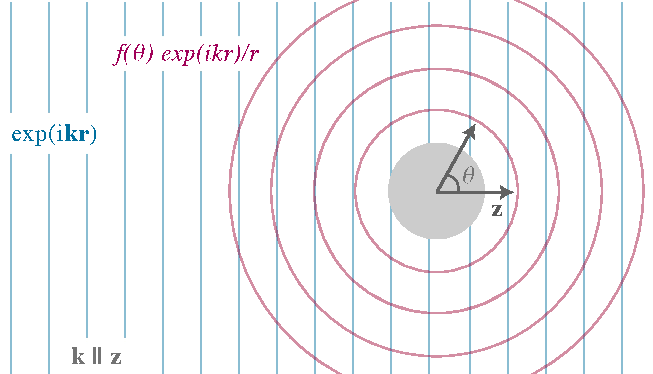
\includegraphics[scale=1]{scattering_scheme}
\decoRule
\caption{ \footnotesize An incoming plane wave scattering off a body making a distorted wave}
\label{fig:scattering_scheme}
\end{figure}

Using the partial wave expansion 
\begin{equation}
\chi^{(+)} \left( {\bf k}, {\bf r} \right) = 
\frac{4 \pi}{kr} \sum_{LM} i^{L} \chi_L \left( k,r \right) 
Y_{LM}\left( \hat{{\bf r}}\right) \left( Y_{LM}( \hat{{\bf k}})\right)^{*},
\end{equation}
A solution for Eq. (\ref{es_she1}) in the absence of any interaction potential, $U \left( r \right) = 0$, is given by 
\begin{equation}
\chi^{(+)} \left( {\bf k}, {\bf r} \right) \rightarrow
e^{i {\bf k} \cdot {\bf r}}, ~~ {\bf r} \rightarrow \infty, 
\end{equation}
for radial part only is written as
\begin{equation}
\chi_L \left( k,r \right)  \rightarrow kr~j_L \left(kr \right),
~~ r \rightarrow \infty,
\end{equation}
where $j_L \left(kr \right)$ is the usual spherical Bessel function. The $\chi_L \left( k,r \right)$ radial function satisfies the radial Shr\"{o}dinger equation
\begin{equation}
\left( \nabla_r + k^2 - \frac{L(L+1)}{r^2} - \frac{2 \mu}{\hbar2} U \left( r \right)\right) \chi_L \left( k,r \right) =0,
\label{es_she_radial}
\end{equation}
where $k^2 = \frac{2\mu E}{\hbar^2}$.

In the case of the interaction potential has a more sophisticated form, including both Coulomb and nuclear short-range  potentials, the radial Shr\"{o}dinger equation (\ref{es_she_radial}) may be rewritten as
\begin{equation}
\left( \nabla_r + k^2 - \frac{2 \eta k}{r} - \frac{L(L+1)}{r^2} - \frac{2 \mu}{\hbar2} U \left( r \right) \right) \chi_L \left( k,r \right) =0,
\label{es_she2}
\end{equation}
where $\eta$ is the usual Sommerfeld parameter with the $Z$ charge numbers
\begin{equation*}
\eta=\frac{Z_a Z_A e^2 \mu}{\hbar^2 k}
\end{equation*}
At the radius $r_0$, where the nuclear potential is negligible, Eq.~(\ref{es_she2}) has the solution, which can be expressed in terms of the $\text{H}_L$ outgoing  and $\text{H}_L^*$ incoming Coulomb functions, as follow
\begin{equation}
\chi_L \left( k,r \right) \rightarrow \frac{i}{2}e^{i \sigma_L} \left( \text{H}_L(kr_0)^*
-S_L \text{H}_L(kr_0)\right), 
~~ r \rightarrow r_0
\label{es_assymp_chi}
\end{equation} 
where $\sigma_L$ is the Coulomb phase shift, and it is given with the $\Gamma$ Gamma function as follow
\begin{equation*}
\sigma_L=Arg\left( \Gamma \left( L+1+i \eta \right) \right)
\end{equation*}
In practice, the radial Eq.~(\ref{es_she2}) is solved by numerical integration from $r \approx 0$, then, matched the value and the slope of the result onto the form (\ref{es_assymp_chi}) ar $r=r_0$. This procedure then gives a value for the $S_L$ scattering matrix elements. Having the $S_L$ matrix elements, the amplitude  of the elastic scattering, analogous  from Eq.~(\ref{es_chi_assymp_with_f}), for the $\chi_L \left( k,r \right)$ wave function in the Eq.~(\ref{es_she2}) is given by
\begin{equation}
f(\theta)=\frac{1}{2ik} \sum_{L} (2L+1) e^{2i\sigma_L} \left( S_L - 1 \right)
\text{P}_L(\text{cos}(\theta))
\label{es_amplitude_nuclear}
\end{equation}
where $\text{P}_L(x)$ is the Legendre polynomials, which are solutions to the Legendre differential equation.
By means of the Rutherford scattering amplitude 
\begin{equation}
f_C(\theta)=-\frac{\eta}{2 k {\text{sin}}^2 \left( \tfrac{1}{2} \theta \right) }
e^{\left( i \eta \text{ln}\left( \text{sin}^2 \left( \tfrac{1}{2} \theta \right) \right)
+2i \sigma_{0} \right)}
\end{equation}
the differential cross section of the elastic scattering has the form
\begin{equation}
\frac{\text{d} \sigma_{\alpha}}{\text{d} \Omega} = \vert f_C(\theta) + f(\theta) \vert^2.
\label{es_diff_cross_section}
\end{equation} 
The expression (\ref{es_diff_cross_section}) allows thus to provide comparison with the obtained  experimental data.   


\section{The coupled channels method for inelastic scattering}
The elastic scattering of the projectile $a$ by the nucleus $A$ has been denoted by $\alpha=a+A$. 
 Let $\alpha^{\prime}=a+A^{*}$ be an inelastic channel , in which only the $A$ nucleus has an extra excitation. In the framework of the coupled channel (CC) approach  the total wave function $\Psi$ for the system may be written as
\begin{equation}
\Psi =  \phi_\alpha \left( { x} \right) \chi_\alpha \left( {\bf r}_\alpha \right)+
\phi_{\alpha^{\prime}}  \left( { x} \right) \chi_{\alpha^{\prime}} \left( {\bf r}_{\alpha^{\prime}} \right)
\label{cc_tot_wf}
\end{equation}
 where ${\bf r}$ is the channel coordinate for the partitions $\alpha$ or $\alpha^{\prime}$, $x$ represents the corresponding internal coordinates.
 The total wave function can be part of the Shr\"{o}dinger equation kind of
 \begin{equation}
 H\Psi=E\Psi
 \label{cc_she1}
 \end{equation}
with the Hamiltonian appropriate particular for the $\alpha$ partition
\begin{equation}
H=H_\alpha + K_\alpha + V_\alpha.
\end{equation}
where $H_\alpha \equiv H_a + H_A$ is the internal Hamiltonian for the nuclei $a$ and $A$, $K_\alpha$ is the kinetic energy operator of relative motion and $V_\alpha$ is the interaction potential operator. The wave functions of ground $ \phi_\alpha \left( { x} \right) $ and excited state $ \phi_{\alpha^{\prime}}  \left( { x} \right)$, being eigenfunctions of the internal Hamiltonian $H_\alpha$
 \begin{align}
H_\alpha  \phi_\alpha \left( { x} \right) =& \varepsilon_\alpha \phi_\alpha \left( { x} \right) \nonumber \\
H_\alpha  \phi_{\alpha^{\prime}} \left( { x} \right) =& \varepsilon_{\alpha^{\prime}} \phi_{\alpha^{\prime}} \left( { x} \right),
 \end{align}
have an orthonormality property  of the form 
\begin{equation}
\int {d x} \left( \phi_\alpha \left( { x} \right)  \right)^{*} \phi_{\alpha^{\prime}} \left( { x}\right) =
\delta_{\alpha \alpha^{\prime}}.
\label{cc_orthonorm}
\end{equation}
 Using the expression of total wave function (\ref{cc_tot_wf}), multiplying Eq.~(\ref{cc_she1}) from the left by the $\phi^{*}_\alpha$ function, then, by the $\phi^{*}_{\alpha^{\prime}}$ function, the two coupled equations can be defined in the following form 
 \begin{align}
\left( E -\varepsilon_\alpha - K_\alpha - \langle \alpha \vert V_\alpha \vert \alpha \rangle \right) \chi_\alpha \left( {\bf r} \right) = & \langle \alpha \vert V_{\alpha} \vert \alpha^{\prime} \rangle \chi_{\alpha^{\prime}} \left( {\bf r} \right) 
\nonumber \\
\left( E -\varepsilon_\alpha - K_\alpha - \langle \alpha^{\prime} \vert V_\alpha \vert \alpha^{\prime} \rangle \right) \chi_{\alpha^{\prime}} \left( {\bf r} \right) =&  \langle \alpha^{\prime} \vert V_{\alpha} \vert \alpha \rangle \chi_{\alpha} \left( {\bf r} \right) 
 \end{align}
where $\langle \alpha \vert V_\alpha \vert \alpha \rangle$, or $\langle \alpha^{\prime} \vert V_{\alpha} \vert \alpha \rangle$, is  the matrix element of $V_\alpha$. In particular,  the matrix element $\langle \alpha^{\prime} \vert V_\alpha \vert \alpha \rangle$ is given by
\begin{align}
\langle \alpha^{\prime} \vert V_\alpha \vert \alpha \rangle = & \int d x \phi_\alpha^{\prime} \left( { x} \right)  V_\alpha \left( x,  {\bf r} \right) \phi_\alpha \left( { x} \right) =\nonumber \\
= & V_{\alpha^{\prime} \alpha} \left(  {\bf r} \right).
\end{align}

An expansion of the coupling potential $V_{\alpha^{\prime} \alpha} \left( {\bf r} \right)$ into the $\lambda$ multipoles can be given as follow
\begin{equation}
V_{\alpha^{\prime} \alpha} \left( {\bf r} \right) = \sum_{\lambda \mu} V^{\lambda \mu}_{\alpha^{\prime} \alpha} (r) Y_{\lambda \mu} \left( \hat{r} \right)
\end{equation}

If the potential shape has a deformation, the nuclear potential can be constructed as
\begin{equation}
V_\alpha \left( x, {\bf r}\right) \equiv U\left( r -\delta\left( \hat{r}^{\prime} \right) \right)
\label{cc_coup_pot_def}
\end{equation}
where $\hat{r}^{\prime}$ denotes angular coordinates of $(\theta,~\phi)$ referred to the intrinsic reference frame. The function $\delta\left( \hat{r}^{\prime} \right)$ is normally expanded in multipoles
\begin{equation}
\delta\left( \hat{r}^{\prime} \right) = \sum_{\lambda} \delta_\lambda Y_{\lambda 0} (\hat{r}^{\prime}).
\label{cc_delta_def}
\end{equation}


In the collective model, the ground and excited states are characterized by their angular momenta $I_i$ and $I_{f}$ with projections $M_i$ and $M_{f}$, respectively. For these state the relevant matrix element of the $V_{\alpha \alpha}^{\lambda \mu}$ operator is described using the Wigner-Eckart theorem by
\begin{equation}
\langle I_{i} M_{i} \vert V^{\lambda \mu}_{\alpha^{\prime} \alpha}  \vert I_f M_f \rangle 
= \sqrt{2I_i + 1} 
\langle I_f M_f \lambda \mu \vert I_i M_i\rangle
 \langle I^{\prime} \vert \vert V^{\lambda}_{\alpha^{\prime} \alpha} \vert \vert	 I \rangle.
 \label{cc_we}
\end{equation} 

Using the definitions, (\ref{cc_coup_pot_def}) and (\ref{cc_delta_def}), the reduced matrix element of radial multipoles from Eq.~(\ref{cc_we}) can be rewritten as follow 
 \begin{equation}
 \langle I_{i} \vert \vert V^{\lambda \mu}_{\alpha^{\prime} \alpha}  \vert \vert I_f \rangle = -\frac{\langle I_{i} \vert \vert \delta_\lambda \vert \vert I_f \rangle}{\sqrt{4 \pi}} 
 \frac{\text{d}U(r)}{\text{d}r}
 \end{equation}
 where 
\begin{equation}
\langle I_{i} \vert \vert \delta_\lambda \vert \vert I_f \rangle = \sqrt{2 I_f+1} 
\langle I_f M_f \lambda 0 \vert I_i M_i \rangle 
\langle \chi \vert \delta \vert \chi \rangle \delta_{M_i M_f}.
\end{equation}
The matrix element $\langle \chi \vert \delta \vert \chi \rangle$ is the expectation value of the operator $\delta_\lambda$ in the internal state of the  deformed nucleus. In the framework of the rotational model it can be given with the deformation length $\beta_\lambda$ as follow
\begin{equation}
\langle \chi \vert \delta \vert \chi \rangle = R_0 \beta_\lambda
\end{equation}
where $R_0$ is an average radius of the interaction potential.

The general asymptotic behaviour of the $\chi_{\alpha}$ elastic channel can be taken from Eq.~(\ref{es_chi_assymp_with_f}), while the inelastic channel $\chi_{\alpha^{\prime}}$ may have 
\begin{equation}
\chi_{\alpha^{\prime}} \left( {\bf r}_{\alpha^{\prime}} \right) \rightarrow 
f_{\alpha^{\prime}} \left( \theta \right)
\frac{e^{i k r_{\alpha^{\prime}}}}{r}, 
~~ {\bf r}_{\alpha^{\prime}} \rightarrow \infty
\end{equation}
Note, that the plane wave expression doesn't not present in this equation - only outgoing wave presents. 
A relevant differential cross section for the inelastic channel is obtained from the coefficient of the outgoing wave as follow
\begin{equation}
\frac{\text{d}\sigma_{\alpha^{\prime}} \left( \theta\right)}{\text{d}\Omega} =
\frac{k_{\alpha^{\prime}}}{k_{\alpha}}
\vert f_{\alpha^{\prime}} \left( \theta \right) \vert^2.
\label{cc_dsigma_domega}
\end{equation}
The wave numbers $k_{\alpha}$ and $k_{\alpha^{\prime}}$ follow from the energy conservation 
\begin{equation}
E=\varepsilon_\alpha + \frac{\hbar^2 k_\alpha}{2 \mu} = 
\varepsilon_{\alpha^{\prime}} + \frac{\hbar^2 k_{\alpha^{\prime}}}{2 \mu}.
\end{equation}

\section{The coupled-reaction-channels method for the transfer reactions}
Consider a model for the $a+A\rightarrow b+B$ nuclear reaction, in which entrance and exit channels are denoted as $\alpha$ and $\beta$ respectively. The $\Psi$ total wave function for this model may be given as
\begin{equation}
\Psi = \chi_{\alpha} \left( {\bf r}_\alpha \right) \phi_\alpha \left( x_\alpha \right) + 
 \chi_{\beta} \left( {\bf r}_\beta \right) \phi_\beta \left( x_\beta \right).
\end{equation}
with a model Hamiltonian $H$ such that $\left( E-H \right) \Psi =0$. From the projections of this equation onto the two channels,
\begin{align}
\langle \chi_\alpha \vert \left( E-H \right) \vert \Psi \rangle = 0 \nonumber \\
\langle \chi_\beta \vert \left( E-H \right) \vert \Psi \rangle = 0
\end{align}
with the two equivalent forms of $H$,
\begin{align}
H= H_\alpha +K_\alpha + V_\alpha \nonumber \\
H= H_\beta +K_\beta + V_\beta
\end{align}
one can get a pair of coupled equations for $\chi_\alpha$ and $\chi_\beta$:
\begin{align}
\left[ ~\left(E-\varepsilon_\alpha \right)  -K_\alpha -
\langle \alpha \vert V_\alpha \vert \alpha \rangle ~\right] 
\chi_\alpha ({\bf r}_\alpha) = 
\langle \alpha \vert H-E \vert  \beta \rangle \chi_\beta \nonumber \\
\left[ ~\left(E-\varepsilon_\beta \right)  -K_\beta -
\langle \beta \vert V_\beta \vert \beta \rangle ~\right] 
\chi_\beta ({\bf r}_\beta) = 
\langle \beta \vert H-E \vert \alpha \rangle \chi_\alpha .
\label{crc_couple_eq1}
\end{align}
These are \textit{the coupled-reaction-channels} (CRC) equations. They are integro-differential equations, as may be seen more explicitly in the form
\begin{align}
\left[ ~\left(E-\varepsilon_\alpha \right)  -K_\alpha -
\langle \alpha \vert V_\alpha \vert \alpha \rangle ~\right] 
\chi_\alpha ({\bf r}_\alpha) = 
\int \text{d} {\bf r}_\beta K_{\alpha \beta} \left( {\bf r}_\alpha, {\bf r}_\beta \right) \chi_\beta \left(  {\bf r}_\beta \right)
 \nonumber \\
\left[ ~\left(E-\varepsilon_\beta \right)  -K_\beta -
\langle \beta \vert V_\beta \vert \beta \rangle ~\right] 
\chi_\beta ({\bf r}_\beta) = 
\int \text{d} {\bf r}_\alpha K_{\beta \alpha} \left( {\bf r}_\beta, {\bf r}_\alpha \right) \chi_\alpha \left(  {\bf r}_\alpha \right)
\end{align}
where the kernels are
\begin{align}
K_{\alpha \beta} \left( {\bf r}_\alpha, {\bf r}_\beta \right) = 
J_{\alpha \beta}
\int \text{d} \zeta_\alpha \phi_\alpha^* \left( x_\alpha \right)
(H-E) \phi_\beta \left( x_\beta \right) \nonumber \\
K_{\beta \alpha} \left( {\bf r}_\beta, {\bf r}_\alpha \right) = 
J_{\beta \alpha}
\int \text{d} \zeta_\beta \phi_\beta^* \left( x_\beta \right)
(H-E) \phi_\alpha \left( x_\alpha \right).
\end{align}
Here the internal coordinates have been transformed from the set $x_\alpha$ to the set $\left( \zeta_\alpha, {\bf r}_\beta \right)$, where the $\zeta_\alpha$ are independent of ${\bf r}_\beta$. Also, $J_{\alpha \beta}$ is the Jacobian of this transformation. Then $J_{\beta \alpha}$ is the Jacobian for the analogous transformation form $x_\beta$ to $\left( \zeta_\beta,{\bf r}_\alpha  \right)$.

Since the off-diagonal matrix elements of $V_\alpha$ are small, they have little effect on the elastic scattering and may be neglected on the right side. 
This implies that the elastic scattering in the entrance $\alpha$ channel is described well by the potential $\langle \alpha \vert V_\alpha \vert \alpha \rangle$, and the potential $\langle \beta \vert V_\beta \vert \beta \rangle$ describes well the elastic scattering in the $\beta$ channel.
%Furthermore, if we have one more channel, it is assumed that all couplings, except the direct coupling to the entrance $\alpha$ channel, can be neglected on the right side of the equation for the $\beta$ channel, so that the potential $\langle \beta \vert V_\beta \vert \beta \rangle$ describes well the elastic scattering in this channel. 
By doing this approximation, Eq.~(\ref{crc_couple_eq1}) may be rewritten as
\begin{align}
\left[ ~\left(E-\varepsilon_\alpha \right)  -K_\alpha -
\langle \alpha \vert V_\alpha \vert \alpha \rangle ~\right] 
\chi_\alpha ({\bf r}_\alpha) \approx & 0
 \nonumber \\
\left[ ~\left(E-\varepsilon_\beta \right)  -K_\beta -
\langle \beta \vert V_\beta \vert \beta \rangle ~\right] 
\chi_\beta ({\bf r}_\beta) \approx &
\langle \beta \vert H-E \vert \alpha \rangle \chi_\alpha
\nonumber \\
\approx &
\langle \beta \vert V_\alpha \vert  \alpha \rangle \chi_\alpha + \langle \beta \vert \alpha \rangle (H_\alpha - E_\alpha) \chi_\alpha 
\nonumber \\
\approx & \langle \beta \vert V_\alpha \vert  \alpha \rangle \chi_\alpha
\label{crc_couple_eq2}
\end{align}
 Here the prior interaction, that is the interaction of the $\alpha$ channel, is used. The non-orthogonal term $\langle \beta \vert \alpha \rangle (H_\alpha - E_\alpha) \chi_\alpha$ vanishes because of the $\chi_\alpha$ is on-shell. The usual Green function techniques may then be used to solve these equations and give \textit{the  distorted wave Born approximation transition} (DWBA) amplitude 
 \begin{align}
 T_{\beta \alpha}^{DWBA} =& \langle \chi_\beta^{(-)} \phi_\beta  \vert V_\alpha \vert
 \chi_\alpha^{(+)} \phi_\alpha \rangle = \nonumber \\
= & \int \int \text{d}x_\beta \text{d}{\bf r}_\beta \chi_\beta^{(-)*} \left( {\bf r}_\beta \right)\phi_\beta^{*} \left( x_\beta \right) V_\alpha 
 \chi_\alpha^{(+)} \left( {\bf r}_\alpha \right)\phi_\alpha \left( x_\alpha \right)
 \end{align}
 where $\chi^{(+)}$ and $\chi^{(-)}$ obey the homogeneous equations
 \begin{align}
 \left[ ~\left(E-\varepsilon_\alpha \right)  -K_\alpha -
\langle \alpha \vert V_\alpha \vert \alpha \rangle ~\right] 
\chi_\alpha^{(+)} ({\bf r}_\alpha) = & 0 \nonumber \\
 \left[ ~\left(E-\varepsilon_\beta \right)  -K_\beta -
\langle \beta \vert V_\beta^{\dagger} \vert \beta \rangle ~\right] 
\chi_\alpha^{(-)} ({\bf r}_\alpha) = & 0 \nonumber
 \end{align}

The differential cross section for the transfer channel $\beta$ can be deduced in the similar way as in Eq.~(\ref{cc_dsigma_domega})

\section{Distorted Wave Born Approximation}

\section{Spectroscopic Amplitudes within the Shell Model}

\section{Interaction potentials. The double folding model}

The numerical calculations  of the elastic scattering  can be performed in the framework of the OM with the OM potential given by:

\begin{equation}\label{eqn:OP}
\begin{array}{l}
 U(R)=-V^{V}(R)-iW^{V}(R)+V^{SO}(R)( \mathbf{l} \cdot \sigma )\\
~~~ ~~~~~~~+V^C(R),
\end{array}
\end{equation}
where $V^{V}, W^{V}, V^{SO},$ and $V^C$ are real volume,  imaginary volume, spin-orbit and Coulomb potentials, respectively. The volume potentials of colliding two spherical nuclei may be represented as parametrized function. For example, in practice the Woods-Saxon potential is often used, and it has the form
\begin{align}
V^V\left( r \right) = & V_0^V f_{r_V, a_V} \left( r \right), \nonumber \\
W^V\left( r \right) = & V_0^W f_{r_W, a_W} \left( r \right), \nonumber \\
f_{r_0, a_0} \left( r \right) = &  \frac{1}{1+ \text{exp} \left( \frac{r-r_0}{a_0} \right) },
\end{align}
where $V_0$ is depth of the potential, $r_0$ is  average distance and $a_0$ is  diffusion parameter. 

%The surface and 
The spin-orbit term of the OM potential has standard form
\begin{eqnarray}
%W^D(R) &= -4 a_D W_0^D \frac{d}{dR} f^{R_D,a_D}(R), \\
V^{SO}(r) &= V_0^{SO}\left(\frac{\hbar}{m_\pi c}\right)^2 \frac{1}{r} \frac{d}{dR} f_{R_{SO} a_{SO}}(r).
\end{eqnarray}
The Coulomb term has been taken as the interaction of a point-charge with a uniformly charged sphere
\[
\label{coul}
V^C(r)=
\begin{cases}
\frac{Z_1 Z_2 e^2}{2 r_C} \left( 3- \frac{r^2}{r_C^2} \right), &\text{  for } r \leq r_C, \\
\frac{Z_1 Z_2 e^2}{r}, & \text{ for } r > r_C .
\end{cases}
\]



The situation changes, when the colliding nuclei have sophisticated shape. Assume, that there are nuclear matter distribution of the projectile $\rho_a \left( { r}_a \right) $ and target $\rho_A \left( { r}_a \right)$, depending on internal their own radii. Folding the nucleon-nucleon interaction potential $V_{nn}$ over the density distributions of nuclear matter, in the framework of \textit{the Double folding model} an interaction potential may be constructed as follow 
\begin{align}
V^V\left( r \right) = & N_f V^{DF} \left( r \right) \nonumber \\ 
V^{DF} \left( {\bf r} \right) = & \int \int \text{d} {\bf r}_a\text{d} {\bf r}_A
\rho_a \left( {\bf r}_a \right) V_{nn} \left( r_{aA}\right)  \rho_A \left( {\bf r}_A \right). 
\label{df_potential}
\end{align}
where $r_{aA}=\vert {\bf r} + {\bf r}_A - {\bf r}_a \vert$ (see Fig.~\ref{fig:df_scheme}). The $N_f$ normalization parameter is usually fitted in accordance with the dynamics of nuclear reaction of elastic scattering.

\begin{figure}
\centering
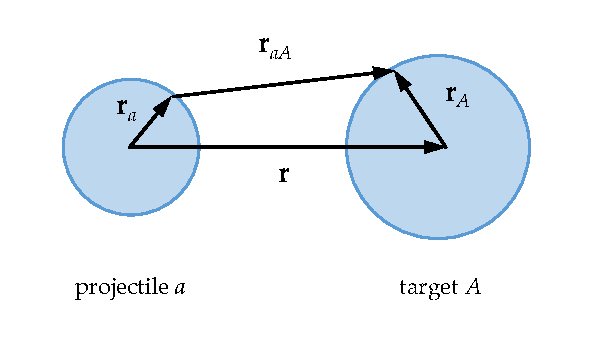
\includegraphics[scale=0.8]{df_scheme}
\decoRule
\caption{ \footnotesize Radius vectors for the double folding model}
\label{fig:df_scheme}
\end{figure}

The DF potential may be calculated using the effective M3Y-Paris \cite{anantaraman1983effective} nucleon-nucleon potential and the nuclear-matter-densities of projectile and target nuclei. 

 The $V_{nn}$ effective nucleon-nucleon interactions usually are taken as a sum of the three Yukawa potentials, i.e. M3Y-potentials:
 % According to Ref. \cite{anantaraman1983effective, bertsch1977interactions}, for both isoscalar and isovector M3Y-potentials have a form as
 \begin{equation}
 V_{nn}(r)=\sum_{i=1}^{3} N_i \frac{\text{exp}(-\mu_i r)}{\mu_i r}.
 \end{equation}
 
 
The parameters  $N_i$, $\mu_i$ of the M3Y-Reid effective NN-potential \cite{bertsch1977interactions}, often used in the double folding calculations, are given in Tab.\ref{m3y_reid_potpar}.
The potential depending on the collision energy of the projectile, undergoes a change by multiplying a factor
\begin{equation}
g(E)= 1-0.002 \frac{E}{A} .
\end{equation}
An additional dependence of the $V_{nn}$ potential on the total density of colliding nuclei in the region of their overlap may given as
\begin{equation}
F(\rho)=C \left( 1+ \alpha \text{exp} \left( - \beta \rho \right) \right).
\label{F_dependence}
\end{equation}
  Studies from Ref. \cite{khoa1994double} has revealed the best agreement of calculated differential cross sections of the $ {}^{12}C+{}^{16}O$  elastic scattering at low and medium energies with the experimental data in conditions, if parameters from Eq.~(\ref{F_dependence}) take the following values: $C=0.2845,~\alpha=3.64, \text{and}~\beta=2.96$.

Another effective potential often used in the double folding calculations is M3Y-Paris \citep{anantaraman1983effective}. 


 For the particles $t$, $^3$He, $\alpha$, which have simple structure, the density distribution of nuclear matter can be represented as parametrized Gaussian function as follow
 \begin{equation}
 \rho \left( r \right) = \rho _0{\mathrm{exp}}\left( - \alpha_0 r^2 \right)
 \end{equation}
 where the parameters $\rho_0$ and $\alpha_0$ are defined in condition to reproduce the rms matter radii
 \begin{equation}
 \alpha_0 = \frac{3}{2\langle r_{m}^{2} \rangle}, 
 \rho_0 = a  \left( \frac{\alpha_0}{\pi} \right)^{3/2}
 \end{equation}
 here $a$ -- atomic number of projectile. 
 %Для ядер $^3$He величина $\langle r^2_m \rangle^{1/2}= 1.703$ фм \cite{pomerantsev2005dibaryon}.
 
 The density distributions in (\ref{df_potential}) are normalized so that
 \begin{align}
 \int \rho_A ({\bf r}) \text{d} {\bf r} & =A \\ \nonumber
 \int \rho_a ({\bf r}) \text{d} {\bf r} & =a
 \end{align}
 where $A, a$ are the number of nucleons in the respective nuclei. 
 
\begin{table*}[bp]
\footnotesize
\caption{\label{m3y_reid_potpar} \footnotesize Parameters of the Reid-Elliot M3Y potential.}
\begin{tabular*}{\textwidth}{lr@{\extracolsep{\fill}}rrrl}
\toprule
$i$ & $N_i$, MeV &  ~ & ~ & ~ &$\mu_i$, $fm^{-1}$ \\
~& Direct T=0~  & Exchange T=0 & Direct T=1 & Exchange T=1&  \\
 \midrule
1  & 7999.0 & 4631.4  & -4885.5 & -1517.9 & 4.0000 	\\
2 & -2134.3  & -1787.1 & 1175.5 & 828.4 & 2.5000  \\ 
3 & 0.0  & -7.8 & 0.0 & 2.6 & 0.7072  \\ 
\bottomrule
\end{tabular*}
\end{table*}
 
 
 
As regards target nuclei, having cluster structure, the density distribution of nuclear matter are calculated by means of the three body wave function, and its details are set out in the next chapter.




\chapter{Results and discussions}
\section{The distribution function of nuclear matter}
Figure \ref{abe_fig2} shows the material densities for the ${}^9$Be nucleus and the components corresponding to the contribution from the $\alpha$ clusters and the valence neutron, calculated using the approach described above as
functions of the radial variable. 
The specific feature of the obtained density is an extended tail at great distances determined by the valence neutron.
The neutron is thus mainly located far from the center of mass
of the system and determines the low binding energy of
${}^9$Be nucleus. 
It is interesting to note that at short distances, the material density of ${}^9$Be has a weak minimum not reported in other works \cite{jansen1972nuclear,fey1973nuclear}.
 Such minima are strongly manifested in stable carbon, nitrogen,
and oxygen isotopes. 
For a ${}^9$Be nucleus considered within the above model, this minimum testifies to its cluster structure and noticeable deformation, reflecting that both the valence neutron and the $\alpha$ clusters are displaced with respect to the common center of mass.


\begin{figure}[bp]
\centering
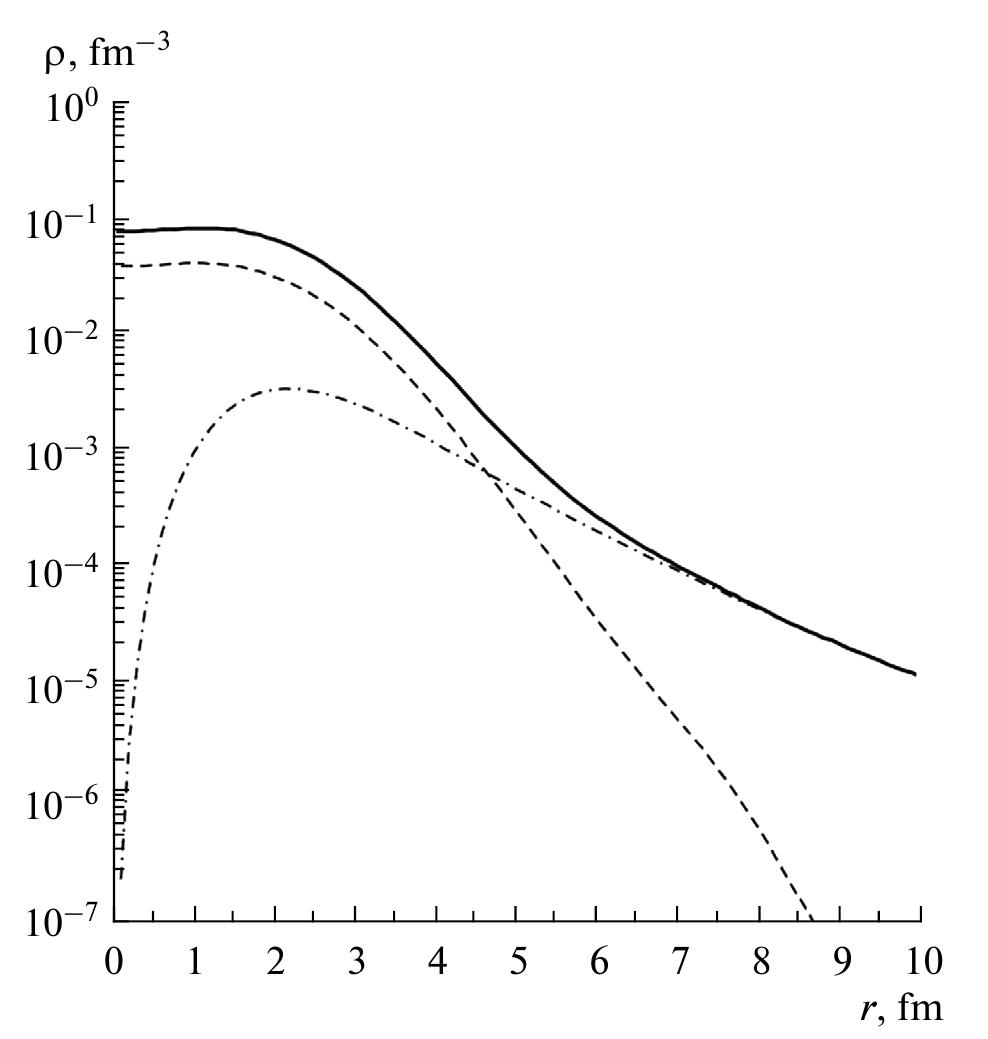
\includegraphics[scale=1]{abe_fig2}
\decoRule
\caption{  \footnotesize  Material density of the ${}^9$Be nucleus as a function of radial variable, calculated using the three cluster model (solid curve). Similar dependences for the $\alpha$ clusters and
the valence nucleon in the ${}^9$Be nucleus are shown by the
dashed and dashed and dotted lines, respectively. }
\label{abe_fig2}
\end{figure}

\section{The $\alpha$ + $^9$Be nuclear reactions}
\subsection{Elastic scattering}
We chose the DDM3YY Paris potential \cite{anantaraman1983effective} as our effective nucleon–nucleon interaction for calculating the folding potential. 
The results from calculating the interaction potential for $\alpha$ and ${}^9$Be nuclei are shown in Fig. \ref{abe_fig3}.
 The depth of the obtained potential on the whole agrees with the known global parameterizations of the optical potential for $\alpha$ nuclei. 
 It should be noted that the potential diffusivity, which is to a large extent determined by the extended spatial distribution of ${}^9$Be (see Fig. \ref{abe_fig2}), is considerable.


\begin{figure}[tp]
\centering
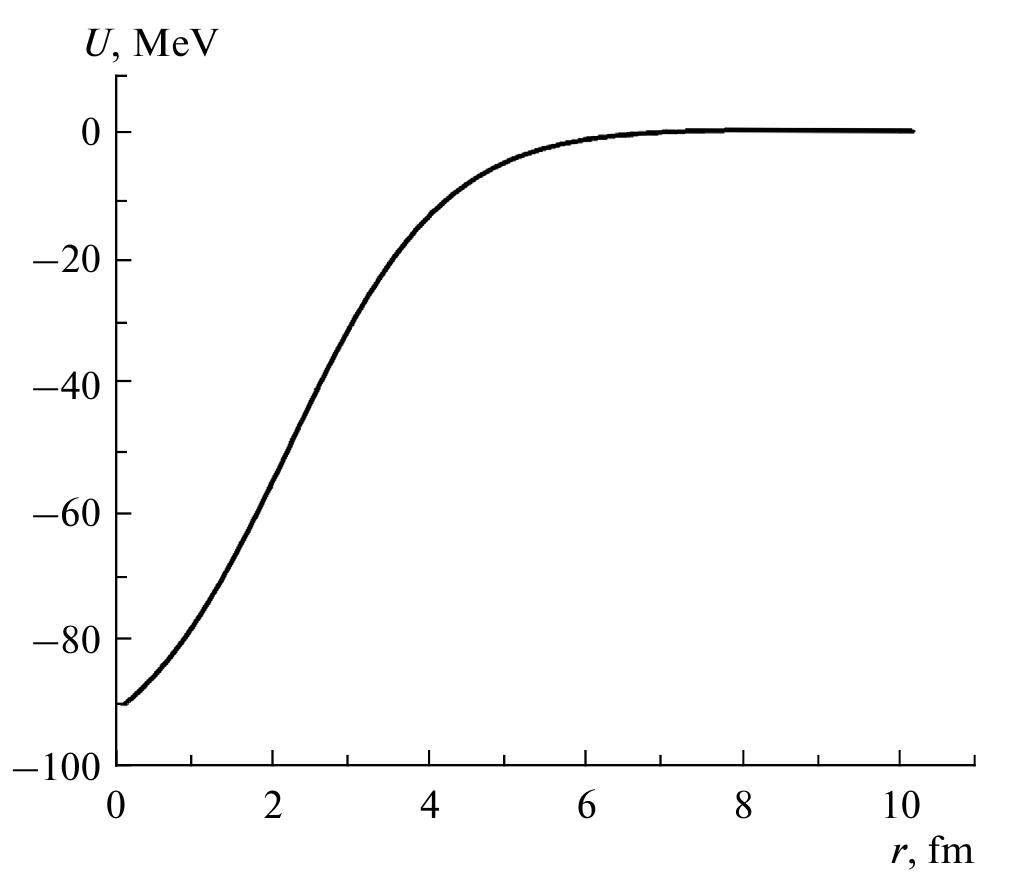
\includegraphics[scale=1]{abe_fig3}
\decoRule
\caption{  \footnotesize  Folding potential of $\alpha$ interaction with $^9$Be nucleus with allowance for the Coulomb interaction.
}
\label{abe_fig3}
\end{figure}


The obtained folding potential was used to calculate the differential cross section of elastic scattering for ${}^9$Be($\alpha$,~$\alpha$)${}^9$Be within the optical model using the data base in \citep{nrv}. 
Figure \ref{abe_fig4} shows the angular distributions obtained in the range of collision energies from 4.5 to 25.1 MeV/nucleon, compared to the available experimental data \cite{lucas1964scattering,burtebaev2002,hauser1969elastic}. 

\begin{figure}[tp]
\centering
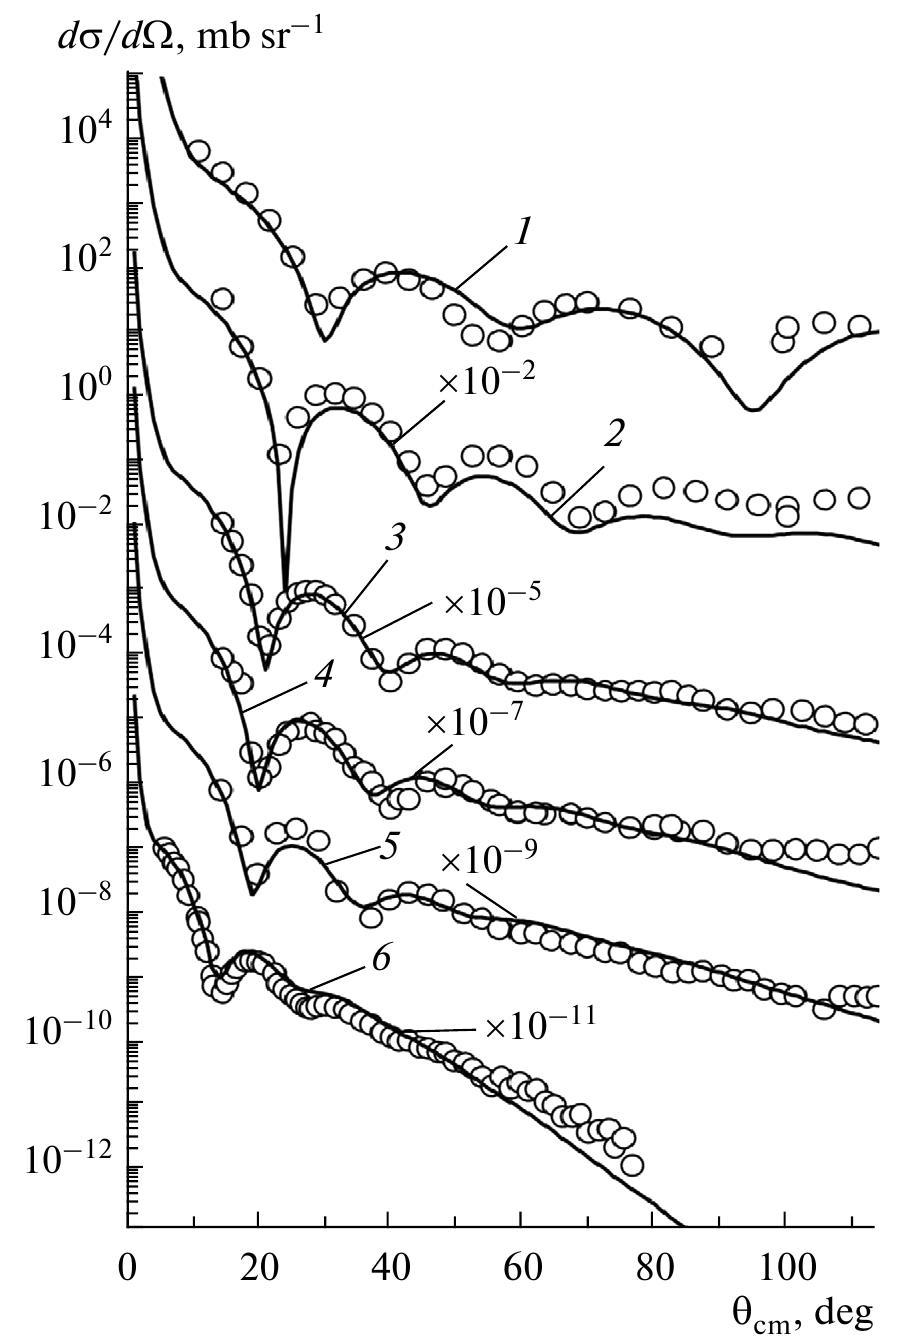
\includegraphics[scale=1]{abe_fig4}
\decoRule
\caption{  \footnotesize   Differential cross sections of elastic scattering ${}^9$Be($\alpha$, $\alpha$)${}^9$Be for different collision energies, compared to the experimental data in \cite{lucas1964scattering,burtebaev2002,hauser1969elastic} : (1) 4.5, (2) 7.25, (3)10.00, (4) 11.25, (5) 12.62, and (6) 26.00 MeV/nucleon.
}
\label{abe_fig4}
\end{figure}


In our calculations, folding potential   was used as the real part of the optical potential  $U_{opt}$ without additional coefficients.
 The optical potential was added using an imaginary term in the form of a Woods–Saxon function with parameters chosen by matching the theoretical cross section to the experimental data (see Table 1).
  The curves in Fig. \ref{abe_fig4} are in good agreement with the data in the region of small and intermediate scattering angles. 
  For large scattering angles at these energies, the elastic scattering cross section is influenced by the mechanism of transfer of heavy $^5$He clusters, which is not explicitly considered in the optical model.

The parameters found for the imaginary part of the optical potential (see Table \ref{abe_tab1}) allow us to study the dependence of the optical potential on the collision energy. In particular, the depth parameter of the imaginary part of the optical potential can be approximately described as
\begin{equation}
W_0(E)=-(23.2+0.15E).
\label{abe_w0}
\end{equation}
The form of the dependence and the found slope coefficient in expression \ref{abe_w0} are in good agreement with the corresponding parameters of the known global parameterizations for optical potentials \cite{avrigeanu1994global}.


\begin{table}[bp]
\caption{
\footnotesize
Parameters of imaginary part of the optical potential for calculating elastic scattering cross section $\alpha$ + $^9$Be. The $a_w$ parameter for all energies is 0.97 fm
}
\label{abe_tab1}
\centering
\footnotesize
\begin{tabular}{lll}
\hline
$E_{lab}$, MeV & $-W_0$, MeV & $r_w$, fm \\ \hline
18             & 26.5        & 1.35      \\
29             & 27.5        & 1.3       \\
40             & 28.5        & 1.25      \\
45             & 30.5        & 1.25      \\
50.5           & 31.5        & 1.1       \\
104            & 39.5        & 1.05      \\ \hline
\end{tabular}
\end{table}

\subsection{Inelastic scattering}
The obtained optical potentials were used to calculate the differential cross sections of inelastic channels within strong channel coupling using the FRESCO code \cite{fresco}. 
%We calculated the excitation cross sections for the low-lying $5/2^{-}$ (2.43 MeV) and $7/2^{-}$ (6.38 MeV) states of the rotational band in $^9$Be nucleus. 
The corresponding angular distributions shown in Fig. \ref{abe_fig5}.a are in good agreement with the experimental data. 
Calculations yield an estimate for the parameter of quadrupole deformation of the target
nucleus:   which is in good agreement with other sources \cite{harakeh1980strong, roy1995coupled, lukyanov2014study}.


\begin{figure}[tp]
\centering
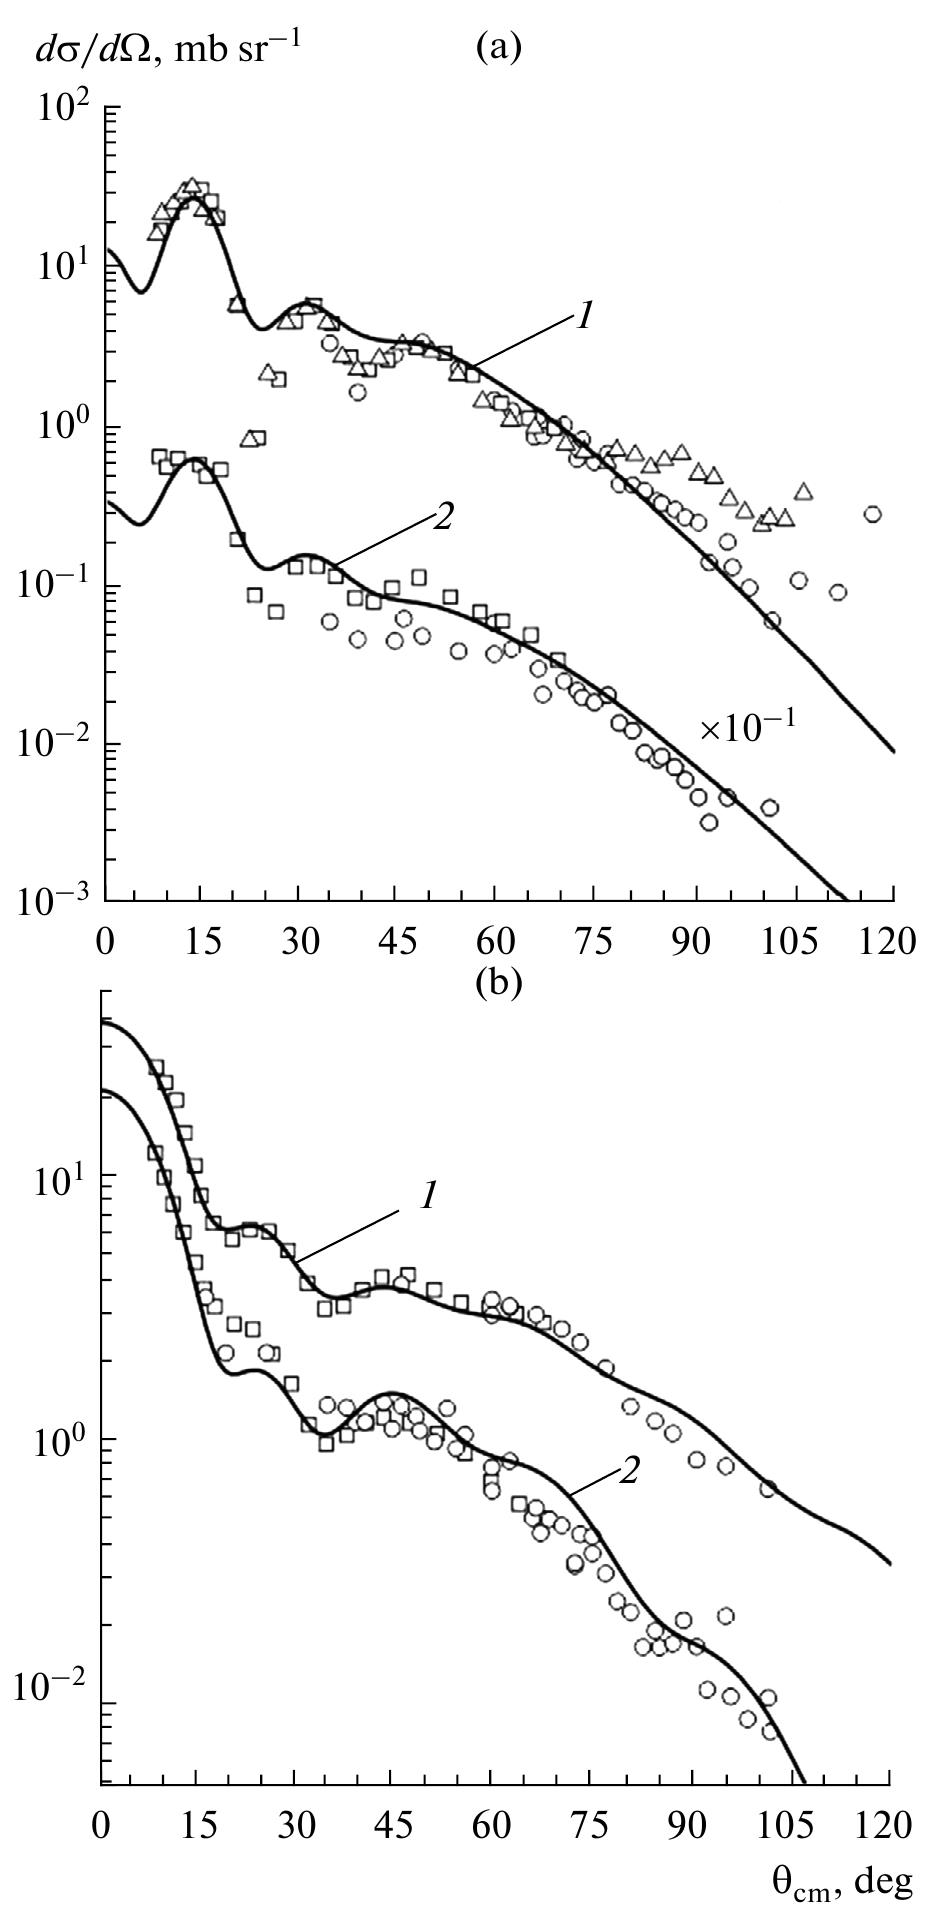
\includegraphics[scale=1]{abe_fig5}
\decoRule
\caption{\footnotesize  Differential cross sections for $E_{lab}$ =16.25 MeV/nucleon: (a) inelastic scattering $^9$Be($\alpha$, $\alpha$)$^9$Be$^*$ with excitation of:  (1) 5/2${}^{-}$ states, (2) 7/2$^{-}$ states; (b) single nucleon transfer reactions: (1)  ${}^{9}$Be($\alpha$, $t$)${}^{10}$B and (2) ${}^{9}$Be($\alpha$,  ${}^{3}$He)${}^{10}$Be. Experimental data are taken from \cite{harakeh1980strong, roy1995coupled, lukyanov2014study}
}
\label{abe_fig5}
\end{figure}


\subsection{One nucleon transfer reactions}
We also calculated the nucleon transfer cross sections within the distorted waves approach using the DWUCK5 code \cite{kunz}. The parameters of the potentials for the input and output reaction channels are given in Table \ref{abe_tab2}. 
Figure \ref{abe_fig5}.b shows the calculated differential cross sections for the transfer reactions ${}^{9}$Be($\alpha$,  ${}^{3}$He)${}^{10}$Be and ${}^{9}$Be($\alpha$, $t$)${}^{10}$B; these describe experimental data quite well. 
A comparison with the measured cross section yields information on the value of the spectroscopic factor   for the ground state of a final nucleus, $^{10}$Be = (${}^{9}$Be + $n$) and $^{10}$B = (${}^{9}$Be + $p$). The obtained values of  ( $^{10}$Be) = 1.1 and  ( $^{10}$B) =
0.6 in particular differ only slightly from the published values \cite{harakeh1980strong, lukyanov2014study, galanina2012mechanisms}. 
The values of the neutron structure factor in ${}^{9}$Be obtained in \cite{galanina2012mechanisms} by analyzing reactions ${}^{9}$Be($d$, $p$)${}^{10}$Be and ${}^{10}$B($d$, $p$)${}^{11}$B are in excellent agreement with the results obtained in this work.

% Please add the following required packages to your document preamble:
% \usepackage{booktabs}
% \usepackage{multirow}
\begin{table}[bp]
\caption{\footnotesize Parameters of the optical potentials for calculations using the distorted waves and channel coupling methods}
\label{abe_tab2}
\centering
\footnotesize
\begin{tabular}{@{}llllllll@{}}
\toprule
$E_{lab}$       & $-V_0$, MeV           & $r_v$, fm             & $a_v$, fm             & $-W_0$, MeV          & $r_w$, fm             & $a_w$, fm             & $r_c$, fm             \\ \midrule
$\alpha+^9$Be   & \multicolumn{3}{l}{The folding potential}                             & 32.65                & 1.14                  & 0.97                  & 1.30                  \\
$^3$He+$^{10}B$ & 132.9                 & 1.54                  & 0.57                  & 19.5                 & 1.82                  & 0.22                  & 0.81                  \\
$t+^{10}$B      & \multirow{2}{*}{95.0} & \multirow{2}{*}{0.95} & \multirow{2}{*}{0.82} & \multirow{2}{*}{8.0} & \multirow{2}{*}{1.60} & \multirow{2}{*}{0.73} & \multirow{2}{*}{1.07} \\
$t+^{10}$Be     &                       &                       &                       &                      &                       &                       &                       \\ \bottomrule
\end{tabular}
\end{table}

\section{The d+$^9$Be nuclear reactions}

\subsection{The elastic channel}
The DF potential was calculated using the effective M3Y-Paris nucleon-nucleon potential and the nuclear-matter-densities of projectile and target nuclei. In order to calculate the ${}^9$Be matter distribution we applied the $\alpha+\alpha+n$ three-body model (for more details, see Ref.~\cite{urazbekov2016}), while the matter density distribution of the deuteron projectile was chosen to be of the form
\begin{equation}
\rho\left( \frac{1}{2}r \right) =\int \vert \Psi (\textbf{r}) \vert ^2 d \Omega_r.
\end{equation}

For convenience, in the OM and CC (CRC) calculations the potentials have been fitted by means of the sum of three Woods-Saxon potentials:
\begin{eqnarray}
V^V(R) =  \sum_{i=1}^{3} V^i f^{R_i, a_i}(R), \\
 f^{R_V,a_V}(R)=\frac{1}{1+exp{\frac{R-R_V}{a_V}}}.
\end{eqnarray}

The parameters of the imaginary part of the optical potential were obtained by fitting the theoretical cross sections to the experimental data at 19.5 MeV and 35 MeV incident energies. As a starting point, the same parameterizations of the real part were used. The obtained potential parameters after fitting are listed in Table~\ref{dbe_potpar} for both 19.5 MeV and 35.0 MeV incident energies.

\begin{figure}[tp]
\centering
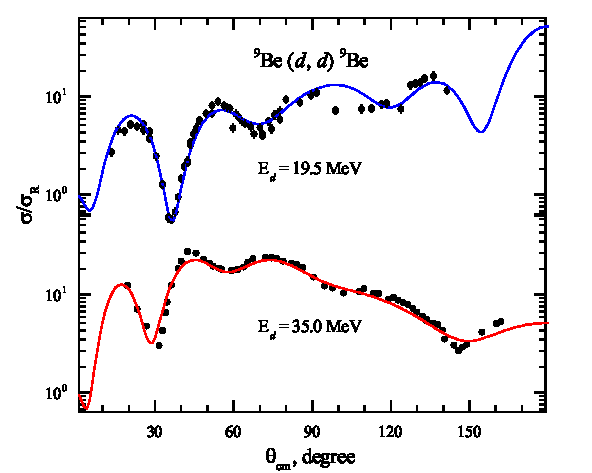
\includegraphics[width=8.2cm]{dbe_fig3.pdf}
\decoRule
\caption{ \label{dbe_fig3} \footnotesize The angular distribution of elastic scattering data of $d$ from ${}^9$Be at laboratory energy 19.5~MeV in comparison with theoretical calculations within the OM (solid curve). }
\end{figure}

The comparison of the results of the theoretical calculations with  the measured data for elastic scattering at 19.5 MeV and 35.0 MeV energies are plotted in Fig.~\ref{dbe_fig3}. 
The cross sections obtained in the framework of the OM with the DF potential are shown as solid curves. 
Theoretical results obtained by means of the OM give an excellent agreement, $\chi^2\approx2.5$, with the experimental data. The  parameters of  parameterized double-folding potential are listed in Table \ref{dbe_potpar}. 

\begin{table*}[bp]
\footnotesize
\caption{\label{dbe_potpar} \footnotesize Parameterized double-folding potentials of the $d$+$^9$Be system used in the OM, CC and DWBA calculations.}
\begin{tabular*}{\textwidth}{ll@{\extracolsep{\fill}}llllllllll}
\toprule
E$_d$, & i & V$_0$, & r$_v^{a}$, & a$_v$, & W$_0$, & r$_w^{a}$, & a$_w$, & V$_0^{SO}$, & N$_R$, & r$_C^{a}$, & $\chi^2/N$ \\
MeV   &   & MeV   & fm    & fm    & MeV   & fm    & fm    & MeV        &       & fm   						& \\ \midrule
19.5  & 1 & 6.18  & 0.328 & 0.308 & 3.99  & 0.328 & 0.127 & 3.275      & 1.22  & 0.809 			& 	2.490	\\
      & 2 & 70.97 & 0.746 & 0.831 & 25.50 (17.5$^{b}$) & 0.746 & 0.766 &            &       &    						&   \\
      & 3 & 0.605 & 1.491 & 1.724 & 0.924 & 1.491 & 2.238 &            &       &   							&    \\ \midrule
35.0  & 1 & 5.941 & 0.328 & 0.308 & 7.07  & 0.612 & 0.108 & 3.275      & 1.17  & 0.809 			&	2.503\\
      & 2 & 68.68 & 0.746 & 0.831 & 22.50 (17.5$^{b}$)& 0.838 & 0.731 &            &       &       						&\\
      & 3 & 0.58  & 1.491 & 1.724 & 0.999 & 1.377 & 1.856 &            &       &      							& \\ \bottomrule
\end{tabular*}
\scriptsize
$^{a}$ Radii are defined as $R_i = r_i \left( A^{1/3}_P+A^{1/3}_T \right)$.  \\
$^{b}$ The values are used in CRC calculations. \\
\end{table*}


\subsection{Inelastic scattering}
The CC and DWBA approaches have been applied to analyse the measured inelastic scattering data corresponding to the ${}^9$Be($5/2^-, 2.43$ MeV) excitation. Calculations were performed employing the FRESCO code \cite{fresco} and the DWUCK5 code \cite{kunz} which are available in the NRV knowledge-base \cite{nrv}.

In order to describe the measured experimental data one has to consider the ${}^9$Be target having a quadrupole deformation. Thus, the ${}^9$Be spectrum consists of the rotational band including the  $3/2^-$ ground state, $5/2^-$ state at 2.43 MeV and $7/2^-$ state at 6.38 MeV. Couplings to these states were taken into account within the coupled-channel approach. The spin reorientations were also taken into account. The coupling interaction has the usual form:
\begin{equation}
V_\lambda(R)=-\beta_\lambda R_V \left|\frac{d V^V}{dR}\right| - i \beta_\lambda R_W \left|\frac{d W^D}{dR}\right|,
\end{equation}
where $\beta_\lambda$ is the deformation parameter of $\lambda$ multipole describing the target-nucleus form. Here, we neglect as usual the contribution of the Coulomb interaction.

\begin{figure}[tp]
\centering
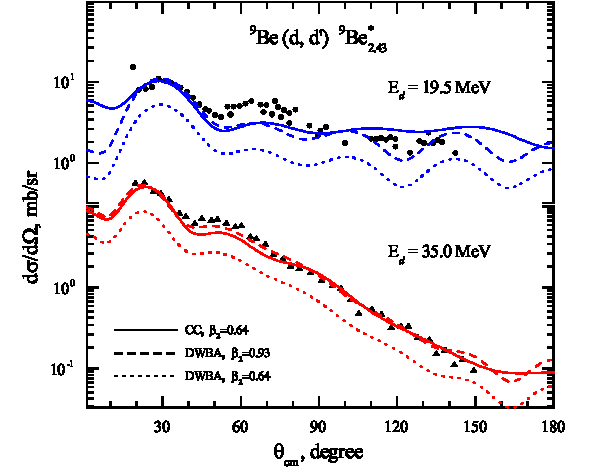
\includegraphics[width=8.2cm]{dbe_fig4.pdf}
\decoRule
\caption{\label{dbe_fig4} \footnotesize The cross sections of inelastic scattering ${}^9$Be($d,d$)$^9$Be* (E$_{exc}$=2.43 MeV) at laboratory energies 19.5 MeV (full circle) and 35 MeV (full triangle). Theoretical curves are described in the text.}
\end{figure} 


\begin{figure}[tp]
\centering
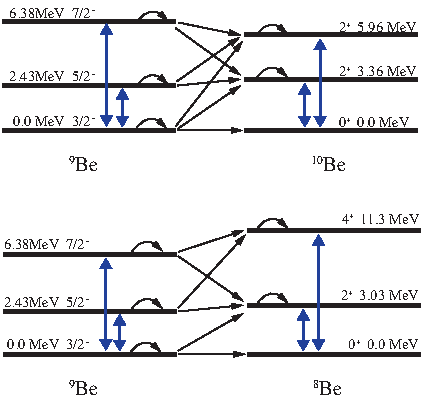
\includegraphics[scale=0.85]{dbe_fig5.pdf}
\decoRule
\caption{ \label{dbe_fig5} \footnotesize The target coupling schemes in the ${}^9$Be($d,p$)$^{10}$Be (upper) and the ${}^9$Be($d,t$)$^8$Be (lower) nuclear reactions. The bold two-headed arrows indicate E$\lambda$ transitions. The spin re-orientation effects are indicated as back-pointing arrows.}
\end{figure} 

The calculated cross sections for inelastic scattering to the $5/2^-$ state at 2.43 MeV are shown in Fig.~\ref{dbe_fig4}. The solid curves correspond to the results obtained within the CC approach, while the dashed and dotted curves were obtained within the DWBA approach using  different values of the deformation parameter $\beta_2$. The used potential parameters are listed in Table~\ref{potpar}.


All the results in Fig.~\ref{dbe_fig4} are in good agreement with the experimental data, except for the cross sections around 60$^\circ$ at 19.5 MeV incident energy. The quadrupole deformation parameter $\beta_2 = 0.64$ extracted within the coupled-channel model is consistent with the previous studies \cite{lukyanov2014study, harakeh1980strong}.

In the case of DWBA calculations, one uses the DF potential (see Table~\ref{dbe_potpar}) for both the entrance and the exit channels. The DWBA angular distributions very well reproduce the structure of experimental data but clearly underestimate them when the deformation parameter $\beta_2 = 0.64$ is used (see the dotted curves in Fig.~\ref{dbe_fig4}). In order to get the best fit the deformation parameter must be increased up to $\beta_2 = 0.93$, which is quite close to the values reported in previous studies (see, for example, \cite{bodek1989, votava1973}).

Thus, one may confirm that channel coupling and the effects of spin reorientation enhance the cross section that results in the reduction of the deformation parameter. However, the DWBA approach takes into account only first-order contributions to the transition amplitude. In particular, it also describes only general features of the angular distributions and overestimates the deformation parameter in order to compensate the difference between the experimental data and the DWBA cross sections.

\subsection{One-nucleon transfer reactions }

The one-neutron pick-up ${}^9$Be($d,t$)${}^8$Be and stripping ${}^9$Be($d,p$)${}^{10}$Be reactions were analyzed here within the framework of  the Coupled Reaction Channels (CRC).

The double-folding potential given in Table \ref{dbe_potpar} was used in the CRC calculations for the entrance channel and the global optical parameterizations from Ref. \cite{globalProton, globalTriton} were used for the exit channels. The coupling schemes of target and daughter nuclei for the ${}^9$Be($d,p$)${}^{10}$Be and ${}^9$Be($d,t$)${}^8$Be  reactions  are illustrated in Fig. \ref{dbe_fig5}. The states of ${}^{10}$Be, $2^+_{1}$ and $2^+_{2}$, as well as the low-lying excited states of ${}^8$Be, $2^+$ and $4^+$, were included in the coupling scheme. Also, the schemes take into account the spin reorientations of states on the condition $J \neq 0$.

In order to construct the bound-state wave functions of the transferred particle in the entrance and exit channels, the common method, i.e. fitting the depth of the corresponding Woods-Saxon potential to the known binding energy, was employed. The reduced radius and diffuseness in this case are set to be $r = 1.25$ fm and $a$ = 0.65 fm, respectively. If the transfer takes place to a final unbound state, the depth of the potential for this state was adjusted to yield a binding energy equal to $-0.1$ MeV in accordance with the procedure used in Ref. \cite{harakeh1980strong}.

\begin{figure}[tp]
\centering
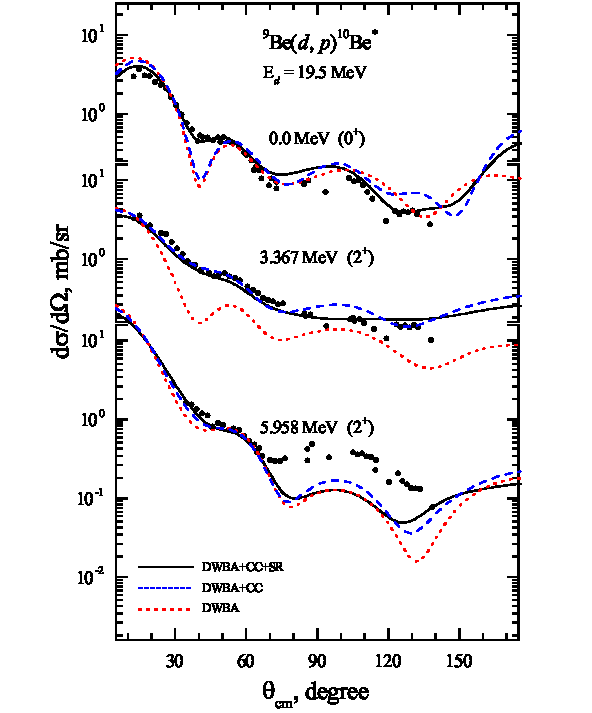
\includegraphics[scale=0.8]{dbe_fig6.pdf}
\decoRule
\caption{\label{dbe_fig6} \footnotesize Differential cross sections for the ${}^9$Be($d,p$)${}^{10}$Be$^*$ reactions at 19.5 MeV leading to different final states (labelled in the figure) in ${}^{10}$Be. The experimental data are shown in comparison with theoretical results obtained within the CRC method.}
\end{figure}

If the core and the composite nuclei have internal excitation energies, a renewed binding energy $BE^{\star}$ of the transferred particle is expressed by the formula:
\begin{equation} BE^{\star}=BE - E_{com}^*+E_{core}^* \end{equation}
where $BE$ $-$ the binding energy of the transferred particle, $E_{com}^*,~E_{core}^*~-$  excitation energies of the composite and  core nuclei, respectively.

\begin{figure}[tp]
\centering
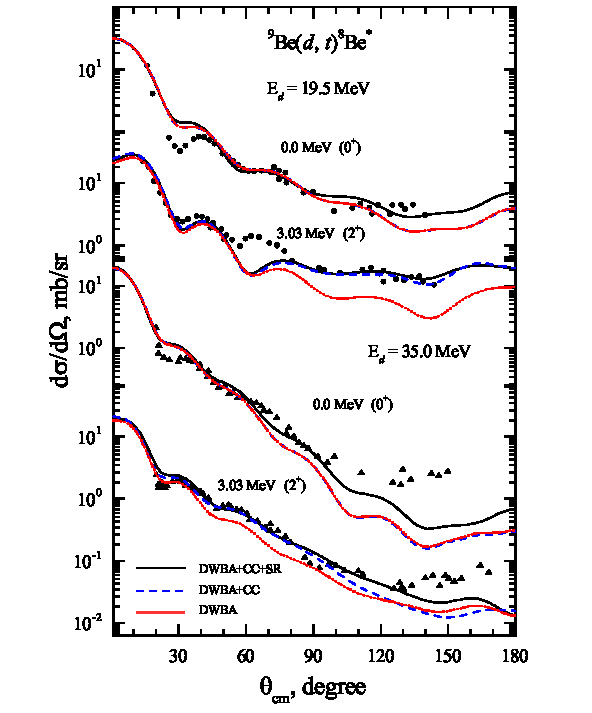
\includegraphics[scale=0.7]{dbe_fig7.pdf}
\decoRule
\caption{
\label{dbe_fig7}
\footnotesize Differential cross sections for the ${}^9$Be($d,t$)${}^{8}$Be$^*$ reactions at 19.5 and 35 MeV leading to different final states (labelled in the figure) in ${}^{8}$Be. The experimental data are shown in comparison with  theoretical results obtained within the CRC method.}
\end{figure}

The spectroscopic amplitude  $\mathcal{S}$ for the addition of a particle to a core with angular momentum $J_{core}$ to form a composite with $J_{com}$ is related to the matrix element of the creation operator~$\hat{a}^\dagger$:
%\cite{brown2017}:
\begin{eqnarray}\label{eq:SA}
\mathcal{S}_{Nlj} = \frac{\langle J_{com} \| \hat{a}^\dagger _{Nlj} \| J_{core}  \rangle}{\sqrt{2J_{com}+1}}
%= (-)^{j+J-J'} \frac{\langle J_{core}  \| \hat{a} _{NL_J} \| J_{com}  \rangle}{\sqrt{2J+1}}
\end{eqnarray}
where $Nlj$ is the set of particle quantum numbers. The spectroscopic amplitudes for one particle states were calculated by means of the $ANTOINE$ code \cite{antoine}  using the effective Cohen-Kurath interaction for $p$-shell nuclei \cite{cohen1965}. The calculated spectroscopic amplitudes for the one-nucleon transfer reactions are listed in Table~\ref{dbe_SA}.

\begin{table*}[tp]
\footnotesize
\caption{\label{dbe_SA} \footnotesize Spectroscopic amplitudes used in CRC calculations for the Composite = Core + Nucleon system. The one-nucleon spectroscopic amplitudes have been calculated by means of the $ANTOINE$ code \cite{antoine}. The alpha spectroscopic amplitudes were taken from  \cite{volya, volya2017}. }
\begin{tabular*}{\textwidth}{@{\extracolsep{\fill}}llllllrl@{\extracolsep{\fill}}llllllr@{\extracolsep{\fill}}}
\toprule
Com & 2J$_{1}$ & Core & 2J$_{2}$ & N & 2J & SA &    & Com & 2J$_{1}$ & Core & 2J$_{2}$ & N & 2J & SA      \\
\midrule 
$^9$Be  & 3  & ${}^8$Be   & 0   & $n$       & 3   & $-$0.761 &  & ${}^9$Be  & 3  & ${}^8$Li   & 2$_1$    & $p$       & 1   & $-$0.444  \\
$^9$Be  & 3  & ${}^8$Be   & 4   & $n$       & 3   & 0.816  &  & ${}^9$Be  & 3  & ${}^8$Li    & 6   & $p$       & 3   & $-$0.592  \\
$^9$Be  & 3  & ${}^8$Be   & 4   & $n$       & 1   & $-$0.242 &  & ${}^9$Be  & 3  & ${}^8$Li    & 2$_2$   & $p$       & 3   & $-$0.236  \\
$^9$Be  & 5  & ${}^8$Be   & 4   & $n$       & 3   & 0.986  &  & ${}^9$Be  & 3  & ${}^8$Li    & 2$_2$   & $p$       & 1   & 0.036   \\
$^9$Be  & 5  & ${}^8$Be   & 4   & $n$       & 1   & $-$0.417 &  & ${}^9$Be  & 5  & ${}^8$Li    & 4   & $p$       & 3   & 0.593   \\
$^9$Be  & 5  & ${}^8$Be   & 8   & $n$       & 3   & $-$0.374 &  & ${}^9$Be  & 5  & ${}^8$Li    & 4   & $p$       & 1   & 0.515   \\
$^9$Be  & 7  & ${}^8$Be   & 4   & $n$       & 3   & $-$0.457 &  & ${}^9$Be  & 5  & ${}^8$Li   & 2$_1$    & $p$       & 3   & $-$0.672  \\
$^9$Be  & 7  & ${}^8$Be   & 8   & $n$       & 3   & 0.919  &  & ${}^9$Be  & 5  & ${}^8$Li    & 6   & $p$       & 3   & $-$0.571  \\
$^9$Be  & 7  & ${}^8$Be   & 8   & $n$       & 1   & $-$0.429 &  & ${}^9$Be  & 5  & ${}^8$Li    & 6   & $p$       & 1   & $-$0.171  \\
$^8$Be  & 0  & ${}^7$Li   & 3   & $p$       & 3   & $-$1.204 &  & ${}^9$Be  & 5  & ${}^8$Li    & 2$_2$   & $p$       & 3   & 0.200     \\
$^8$Be  & 0  & ${}^7$Li   & 1   & $p$       & 1   & 0.736  &  & ${}^9$Be  & 7  & ${}^8$Li    & 4   & $p$       & 3   & $-$0.323  \\
$^8$Be  & 4  & ${}^7$Li   & 3   & $p$       & 3   & $-$0.748 &  & ${}^9$Be  & 7  & ${}^8$Li    & 6   & $p$       & 3   & $-$0.899  \\
$^8$Be  & 4  & ${}^7$Li   & 3   & $p$       & 1   & $-$0.612 &  & ${}^9$Be  & 7  & ${}^8$Li    & 6   & $p$       & 1   & $-$0.564  \\
$^8$Be  & 4  & ${}^7$Li   & 1   & $p$       & 3   & 0.667  &  & ${}^7$Li  & 3  & ${}^6$Li   & 2   & $n$       & 3   & 0.657   \\
$^8$Be  & 4  & ${}^7$Li   & 7   & $p$       & 3   & 0.624  &  & ${}^7$Li  & 3  & ${}^6$Li   & 2   & $n$       & 1   & $-$0.538  \\
$^8$Be  & 4  & ${}^7$Li   & 5$_2$   & $p$       & 3   & 0.079  &  & ${}^7$Li  & 3  & ${}^6$Li   & 6   & $n$       & 3   & 0.744   \\
$^8$Be  & 4  & ${}^7$Li   & 5$_2$   & $p$       & 3   & $-$0.146 &  & ${}^7$Li  & 3  & ${}^6$Li   & 4   & $n$       & 3   & $-$0.032  \\
$^8$Be  & 8  & ${}^7$Li   & 7   & $p$       & 3   & 0.864  &  & ${}^7$Li  & 3  & ${}^6$Li   & 4   & $n$       & 1   & 0.399   \\
$^8$Be  & 8  & ${}^7$Li   & 7   & $p$       & 1   & 0.687  &  & ${}^7$Li  & 1  & ${}^6$Li   & 2   & $n$       & 3   & $-$0.925  \\
$^8$Be  & 8  & ${}^7$Li   & 5$_2$   & $p$       & 3   & 0.374  &  & ${}^7$Li  & 1  & ${}^6$Li   & 2   & $n$       & 1   & 0.197   \\
$^8$Li  & 4  & ${}^7$Li   & 3   & $n$       & 3   & $-$0.988 &  & ${}^7$Li  & 1  & ${}^6$Li   & 4   & $n$       & 3   & $-$0.555  \\
$^8$Li  & 4  & ${}^7$Li   & 3   & $n$       & 1   & 0.237  &  & ${}^7$Li  & 7  & ${}^6$Li   & 6   & $n$       & 3   & $-$0.936  \\
$^8$Li  & 4  & ${}^7$Li   & 1   & $n$       & 3   & 0.430   &  & ${}^7$Li  & 7  & ${}^6$Li   & 6   & $n$       & 1   & 0.645   \\
$^8$Li  & 4  & ${}^7$Li   & 7   & $n$       & 3   & $-$0.496 &  & ${}^7$Li  & 7  & ${}^6$Li   & 4   & $n$       & 3   & $-$0.456  \\
$^8$Li  & 4  & ${}^7$Li   & 5   & $n$       & 3   & $-$0.665 &  & ${}^7$Li  & 5$_2$  & ${}^6$Li   & 2   & $n$       & 3   & $-$0.650   \\
$^8$Li  & 4  & ${}^7$Li   & 5$_2$   & $n$       & 1   & $-$0.275 &  & ${}^7$Li  & 5$_2$  & ${}^6$Li   & 6   & $n$       & 3   & 0.732   \\
$^8$Li  & 2$_1$  & ${}^7$Li   & 3   & $n$       & 3   & 0.567  &  & ${}^7$Li  & 5$_2$  & ${}^6$Li   & 6   & $n$       & 1   & 0.549   \\
$^8$Li  & 2$_1$  & ${}^7$Li   & 3   & $n$       & 1   & 0.351  &  & ${}^7$Li  & 5$_2$  & ${}^6$Li   & 4   & $n$       & 3   & 0.200     \\
$^8$Li  & 2$_1$  & ${}^7$Li   & 1   & $n$       & 3   & 0.905  &  & ${}^7$Li  & 5$_2$  & ${}^6$Li   & 4   & $n$       & 1   & $-$0.114  \\
$^8$Li  & 2$_1$  & ${}^7$Li   & 1   & $n$       & 1   & 0.331  &  & ${}^6$Li  & 2  & $d$     & 2   & $\alpha$     & 0   & 0.907  \\
$^8$Li  & 2$_1$  & ${}^7$Li   & 5$_2$   & $n$       & 3   & 0.767  &  & ${}^6$Li  & 2  & $d$     & 2   & $\alpha$     & 4   & 0.077   \\
$^8$Li  & 6  & ${}^7$Li   & 3   & $n$       & 3   & 0.581  &  & ${}^6$Li  & 6  & $d$     & 2   & $\alpha$     & 4   & 0.943   \\
$^8$Li  & 6  & ${}^7$Li   & 5$_2$   & $n$       & 3   & $-$0.660  &  & ${}^6$Li  & 6  & $d$     & 2   & $\alpha$     & 8   & 0.028   \\
$^8$Li  & 6  & ${}^7$Li   & 5$_2$   & $n$       & 1   & $-$0.541 &  & ${}^6$Li  & 4  & $d$     & 2   & $\alpha$     & 4   & 0.929   \\
$^8$Li  & 6  & ${}^7$Li   & 7   & $n$       & 3   & 0.973  &  & ${}^9$Be  & 3  & ${}^5$He   & 3   & $\alpha$     & 0   & $-$0.925  \\
$^8$Li  & 6  & ${}^7$Li   & 7   & $n$       & 1   & $-$0.404 &  & ${}^9$Be  & 3  & ${}^5$He   & 3   & $\alpha$     & 4   & 0.784   \\
$^8$Li  & 2$_2$  & ${}^7$Li   & 3   & $n$       & 3   & $-$0.617 &  & ${}^9$Be  & 5  & ${}^5$He   & 3   & $\alpha$     & 4   & 0.974   \\
$^8$Li  & 2$_2$  & ${}^7$Li   & 3   & $n$       & 1   & $-$0.841 &  & ${}^9$Be  & 5  & ${}^5$He   & 3   & $\alpha$     & 8   & $-$0.260   \\
$^8$Li  & 2$_2$  & ${}^7$Li   & 1   & $n$       & 3   & 0.178  &  & ${}^9$Be  & 7  & ${}^5$He   & 3   & $\alpha$     & 4   & 0.882   \\
$^8$Li  & 2$_2$  & ${}^7$Li   & 1   & $n$       & 1   & 0.331  &  & ${}^9$Be  & 7  & ${}^5$He   & 3   & $\alpha$     & 8   & $-$0.737  \\
$^8$Li  & 2$_2$  & ${}^7$Li   & 5   & $n$       & 3   & 0.231  &  & ${}^7$Li  & 3  & $t$     & 1   & $\alpha$     & 1   & 0.970       \\
$^9$Be  & 3  & ${}^8$Li    & 4   & $p$       & 3   & $-$0.947 &  & ${}^7$Li  & 1  & $t$     & 1   & $\alpha$     & 1   & 0.961       \\
$^9$Be  & 3  & ${}^8$Li    & 4   & $p$       & 1   & $-$0.319 &  & ${}^7$Li  & 7  & $t$     & 1   & $\alpha$     & 3   & 0.952       \\
$^9$Be  & 3  & ${}^8$Li    & 2$_1$   & $p$       & 3   & 0.454  &  & ${}^7$Li  & 5$_2$  & $t$     & 1   & $\alpha$     & 3   & 0.223  \\
\bottomrule
\end{tabular*}
\end{table*}

Angular distributions of the ${}^9$Be($d,p$)${}^{10}$Be nuclear reaction at E$_d$=19.5 MeV are shown in comparison with the theoretical curves  calculated in the framework of the CRC method in Fig. \ref{dbe_fig6}.

In order to study the couplings of the input  channels, the outputs  were fixed using the deformation parameter of $^8$Be from Ref. \cite{rocca2018}, and for $^{10}$Be from Ref. \cite{harakeh1980strong}. 
The direct transition from the ground state is indicated by the dotted line (DWBA). 
The contributions of the transitions from excited states (CC), and from spin reorientations (SR) are indicated by dashed and solid lines, respectively.
During the analysis, it was found that spin reorientation has a significant contribution in the $p$ + $^{10}$Be$_{gs}$ channel, especially in the range of 40-60 degrees. 

It is interesting to note that we managed to describe within the CRC method the differential cross section of the ${}^9$Be($d,p$)${}^{10}$Be$_{gs}$ reaction at all scattering angles, including the range 40$^\circ$-60$^\circ$, where they were not covered in Refs. \cite{galanina2012, bodek1989}.
 
An appreciable contribution of the \begin{small}
$3/2^- \rightarrow 2^+_1,~5/2^- \rightarrow 2^+_1,~7/2^-\rightarrow 2^+_1$
\end{small} transitions was observed in the $p$~+~$^{10}$Be$_{3.37}$ channel in the entire range of scattering angles. 
In the cross section of the  $p$~+~$^{10}$Be$_{5.96}$ channel, the theoretical calculation underestimates the experimental data starting from 70$^\circ$. Possibly, other higher excited states of $^9$Be should be taken into account.

Figure \ref{dbe_fig7} displays the cross sections of the ${}^9$Be($d,t$)${}^{8}$Be nuclear reaction at both 19.5 MeV and 35 MeV incident energies. As in the case of the ($d,p$) reactions, the ($d,t$) reactions also show the strong channel-coupling effects. We see a manifestation of spin-reorientation effects in the $t$+$^8$Be$_{gs}$ channels and a significant contribution of the  \begin{small}
$3/2^- \rightarrow 2^+,~ 5/2^- \rightarrow 2^+,~ 7/2^-\rightarrow 2^+$
\end{small} transitions in the $t$+$^8$Be$_{3.03}$ channel.
Disagreements around 30$^\circ$ in the $t$+$^8$Be$_{gs}$ channel for both 19.5 MeV and 35 MeV incident energies and around 60$^\circ$ in the $t$+$^8$Be$_{3.03}$ channel for 19.5 MeV incident energy are possibly caused by the uncertainty in the $t$+$^8$Be interaction potential.

Theoretical calculations made within the CRC method show, in general, good agreement with the experimental data for both ($d,p$)  and ($d,t$) reactions.
The analysis showed strong coupling effects in both entrance and exit channels. The effects of such couplings were also emphasized in Refs. \cite{harakeh1980strong, rudchik2016}.

\subsection{Cluster-transfer reaction}
Differential cross sections for the nuclear reaction ${^9}$Be($d,\alpha$)${}^7$Li are of particular interest. This is due to the specific behaviour of the cross section at large scattering angles, which indicates a ${}^5$He cluster transfer. In addition, the cross section calculated within the DWBA approach underestimates the data even at forward scattering angles. Therefore, in order to understand the difference between theory and experiment, the following transfer mechanisms are suggested (see Fig. \ref{dbe_fig9}):
\begin{itemize}
\item[$-$] direct transfer of heavy clusters $d$ and ${}^5$He;
\item[$-$] sequential two-step transfer of $n$-$p$, $p$-$n$, $n$-$\alpha$ and $\alpha$-$n$;
\end{itemize}


\begin{figure}[tp]
\centering
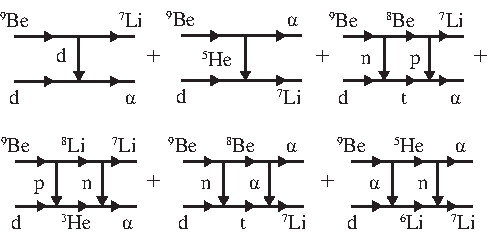
\includegraphics[width=8.2cm]{dbe_fig9.pdf}
\decoRule
\caption{\label{dbe_fig9} \footnotesize The scheme illustrates the reaction mechanisms taken into account in CRC calculations of the cross sections for ${}^9$Be($d,\alpha$)${}^7$Li reaction.}
\end{figure}


The resulting differential cross section for the ${^9}$Be($d$,$\alpha$)${}^7$Li reaction has the form of a coherent sum of two amplitudes
\begin{equation}
\frac{d\sigma}{d\Omega}(\theta) =\vert f_{I}(\theta) + f_{II}(\theta) \vert ^2,
\end{equation}
where the amplitude
\begin{equation} \label{eq:ampl1}
f_{I}(\theta)=f_{{}^5\textrm{He}}(\pi - \theta) + f_{n\textrm{-}\alpha}(\pi - \theta) + f_{\alpha\textrm{-}n}(\pi - \theta)
\end{equation}
describes the transfer of the heavy ${}^5$He-cluster and sequential two-step transfer of n-$\alpha$ and $\alpha$-n, and the amplitude
\begin{equation} \label{eq:ampl2}
f_{II}(\theta)=f_{d}(\theta) + f_{n\textrm{-}p}( \theta) + f_{p\textrm{-}n}(\theta)
\end{equation}
corresponds to the deuteron pick-up and sequential two-step transfer of $n$-$p$ and $p$-$n$.


\begin{figure*}[tp]
\centering
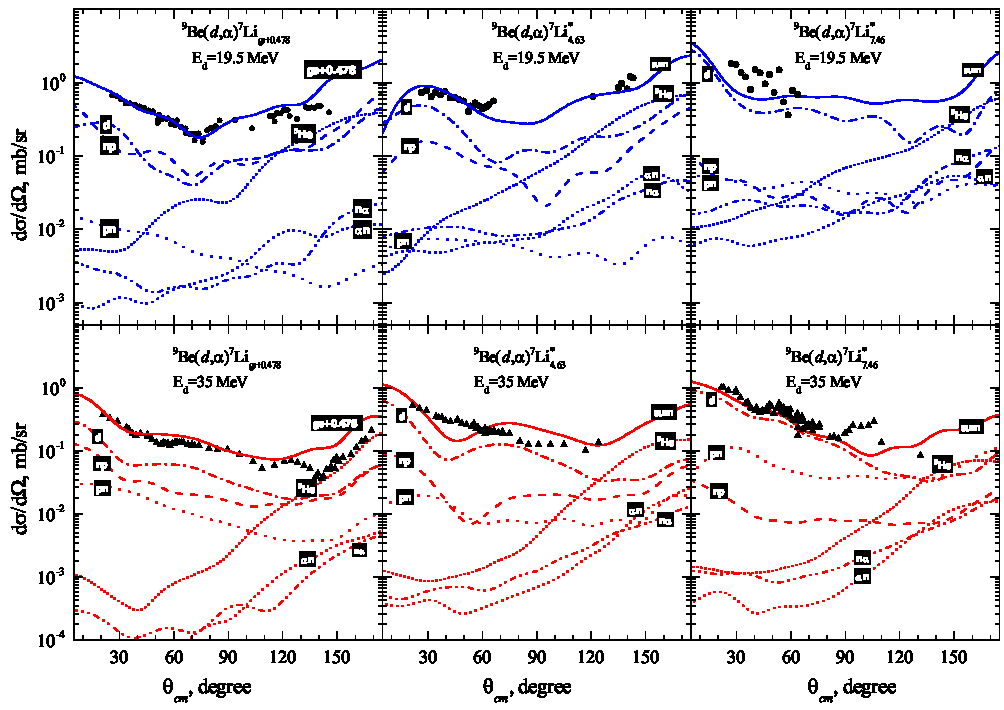
\includegraphics[scale=0.8]{dbe_fig8.pdf}
\decoRule
\caption{ \footnotesize Differential cross sections for the ${}^9$Be($d$,$\alpha$)${}^7$Li reactions measured at 19.5 MeV and 35 MeV energy with the ${}^{7}$Li observed in the ground or low-lying excited states in the exit channels.}
\label{dbe_fig8}
\end{figure*}	


The DF potential (see Table~\ref{dbe_potpar}) for the entrance channel and global optical potential parameterizations from Refs. \cite{globalTriton, globalAlpha, global6Li} for intermediate and exit channels were used in the analysis.
The prior form for the first coupling and the post form for the second coupling were chosen for two-step transfer reactions in order to avoid the non-orthogonal terms in the calculations of transition amplitudes.

%Important ingredients of the CRC method are the spectroscopic amplitudes of the composite configurations in the entrance, exit and intermediate states. In order to calculate the one nucleon spectroscopic amplitudes we applied the \textit{ANTOINE} code \cite{antoine} that reproduces the excitation functions of all p-shell nuclei well.

The spectroscopic amplitudes of the $d$ and ${}^5$He clusters were taken from Ref. \cite{fiveSA}, while the alpha-cluster spectroscopic amplitudes given in Table~\ref{dbe_SA} were provided by Dr. A. Volya within the method reported in Ref. \cite{volya2017}.

The calculated cross sections are shown in Fig.~\ref{dbe_fig8} with the $\alpha$-particle angular distributions formed in the ${}^9$Be(d,$\alpha$)${}^7$Li$^*$ reaction at incident energies of 19.5 and 35 MeV and corresponding to the low-lying excitation of the ${}^7$Li nucleus in the exit channels. The transfer of the deuteron (dash-dotted curve) provides the dominant contribution in all the channels. Despite the fact that the spectroscopic amplitude of the deuteron $\mathcal{S}_{1{D}_3}=0.558$ in the ${}^9$Be nucleus is not of great importance, a noticeable cross section is due to the large value of the deuteron spectroscopic amplitude $\mathcal{S}_{1{S}_1}=1.732$  of ${}^4$He.

The angular distribution of deuteron transfer has a significant cross section also at the backward scattering angles, which is mainly caused by the contribution of the $D$ wave. This symmetrical behaviour of the cross section of $D$ waves is very similar to the cross section of evaporation residues. Tanaka \textit{et al} \cite{tanaka1978} analyzed the role of the compound process in ${}^9$Be($d,\alpha$)${}^7$Li reaction and claimed the domination of the compound nucleus channels at the energies of 12.17 MeV and 14.43 MeV. However, in Ref. \cite{bodek1989} the negligible contribution of the compound-nucleus mechanism was shown at 7 MeV using the DWBA analysis. In this regard, our theoretical results based on the CRC method show that there is no need to take into account the mechanism through the compound-nucleus formation at energies of 19.5 and 35.0 MeV.

Starting from scattering angle $\theta_{c.m.} =$ 120$^\circ$, the transfer of the ${}^5$He cluster, labeled as ${}^5$He in Fig. \ref{dbe_fig8}, has a predominant contribution in all channels. It should be noted that a similar result was reported earlier in Ref. \cite{bodek1989}. One-step transfer of the ${}^5$He cluster was also indicated as a dominant process by Jarczyk \textit{et al} \cite{jarczyk1996} in studying the ${}^{12}$C(${}^{11}$B,${}^6$Li)${}^{17}$O and ${}^{12}$C($d$,${}^7$Li)${}^{7}$Be reactions.

Using the CRC method, we are able to estimate the contribution of the sequential transfer of ${}^5$He, which was not studied before. Corresponding cross sections are shown in Fig.~\ref{dbe_fig8} as curves labeled $n\alpha$ and $\alpha n$.
It turned out that the $n$-$\alpha$ and $\alpha$-$n$ transfer processes provide indeed a contribution more than one order of magnitude smaller in comparison with the one-step ${}^5$He transfer. Nevertheless, it should be noted that the contribution of the $n$-$\alpha$ and the $\alpha$-$n$ transfer channels increases with the increase in the ${}^7$Li excitation energy, where they should not be ignored.

\begin{figure}%[tp]
\centering
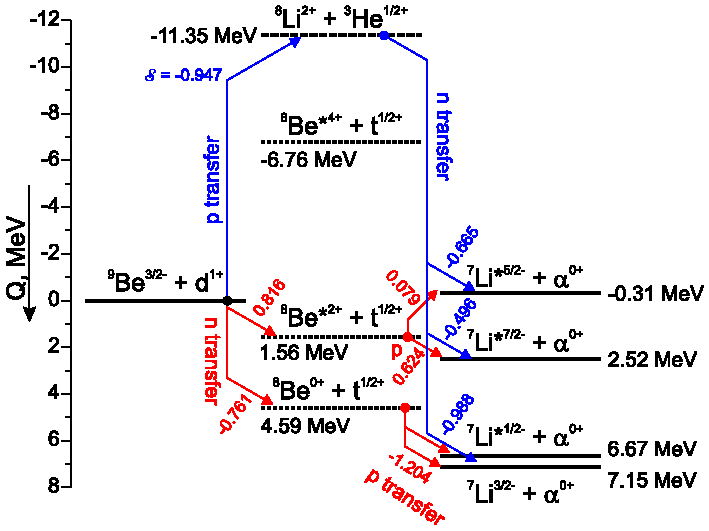
\includegraphics[width=8.2cm]{dbe_fig10.pdf}
\decoRule
\caption{\label{dbe_fig10} \footnotesize The scheme illustrates the energy balance of the different intermediate stages for the two-step mechanisms of ${}^9$Be($d,\alpha$)${}^7$Li transfer reaction. The $Q$-values for the different intermediate channels are shown near the corresponding lines. The numbers near the arrows correspond to the spectroscopic amplitudes of the heaviest reaction participants. For example, spectroscopic amplitude for the ${}^9$Be = ${}^8$Li + $p$ configuration is equal $\mathcal{S} = -0.947$.}
\end{figure}

The two-step $n$-$p$ transfer is another mechanism providing a noticeable contribution to the cross section. It is due to the prominent cluster structure of the ${}^9$Be nucleus having the weakly bound neutron. This structural feature explains also the weakness of the $p$-$n$ sequential transfer contribution to the cross section corresponding to the ${}^7$Li(g.s.) in the exit channel. However, with increasing the ${}^7$Li excitation energy these two mechanisms are interchanged in the significance of their contributions, as depicted by the curves in Fig.~\ref{dbe_fig8}, and the $p$-$n$ transfer begins to play a leading role, providing, in particular, almost 10 times larger contribution in the case of reaction at $E_{lab}$ = 35 MeV with ${}^7$Li$^*$(7.46 MeV) in exit channel.

In Fig.~\ref{dbe_fig10}, the possible scenarios for the $n$-$p$ and $p$-$n$ sequential transfer for the reaction under consideration are shown in respect to the $Q$-values. One may see that all the steps of the $n$-$p$ sequential transfer have positive $Q$-values, while the $p$-$n$ transfer goes through the intermediate channel ${}^8$Li + ${}^3$He that has a considerably negative $Q$-value. Together with the large values of the spectroscopic amplitudes (shown near to the arrows in Fig. \ref{dbe_fig10}), this explains the leading role of the ($d,t;t,\alpha$) mechanism in populating the ground state of ${}^7$Li in the exit channel.

\begin{figure}[tp]
\centering
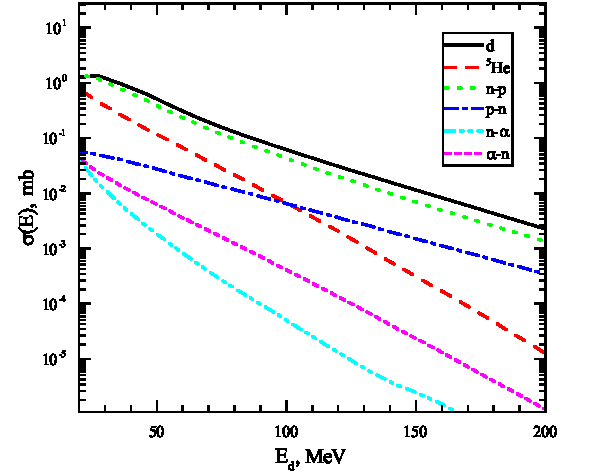
\includegraphics[width=8.2cm]{dbe_fig11.pdf}
\decoRule
\caption{\label{dbe_fig11} \footnotesize Contributions of the different mechanisms to the cross section of the ${}^9$Be($d,\alpha$)${}^7$Li$_{g.s.}$ reaction. See Fig.~\ref{dbe_fig9} for explanation of the curve notations.}
\end{figure}	

The situation becomes quite different in the case of the ${}^7$Li$^*$(5/2$^-$) in the exit channel. First, the population of this state through the $n$-$p$ transfer involves the ${}^9$Be~=~${}^8$Be$^*(2^+)$~+~$n$ intermediate configuration where the ${}^8$Be cluster has to be in the $2^+$ excited state. Note that the ${}^8$Be($0^+$) ground state is inappropriate because of angular-momentum-coupling mismatch in the entrance and exit configurations. Second, the extremely small spectroscopic amplitude of the ${}^8$Be$^*(2^+)$~=~${}^7$Li$^*(5/2^-)$~+~$p$ configuration, which is $\mathcal{S} = 0.079$, influences the transfer amplitude. These two factors lead to the suppression of the contribution of ($d,t;t,\alpha$) mechanism in population of the ${}^7$Li$^*$(5/2$^-$) state in the exit channel. Therefore, the $p$-$n$ sequential transfer prevails over the $n$-$p$ one. 

Figure \ref{dbe_fig11} shows the contributions of all the mechanisms mentioned above to the total cross section of the ${}^9$Be($d,\alpha$)${}^7$Li$_{g.s.}$ reaction (see Fig.~\ref{dbe_fig9}) as a function of the deuteron energy. One may conclude that mainly four mechanisms contribute to the cross section of this reaction. The transfer of the deuteron-cluster is the predominant channel at all collision energies. The sequential $n$-$p$ and $p$-$n$ transfers play a significant role at the high energies. The ${}^5$He-cluster transfer gives almost 20\% of the cross section at low energies and outdoes the sequential $p$-$n$ transfer in this energy domain. This allows us to claim that the configurations $n+^8$Be and $\alpha+{}^5$He provide noticeable contributions to the ground-state wave function of the ${}^9$Be nucleus. These conclusions agree well with the previous experimental studies \cite{brown2007, papka2007}.


\chapter{Conclusion}
%\include{Chapters/Chapter2} 
%\include{Chapters/Chapter3}
%\include{Chapters/Chapter4} 
%\include{Chapters/Chapter5} 

%----------------------------------------------------------------------------------------
%	THESIS CONTENT - APPENDICES
%----------------------------------------------------------------------------------------

\appendix % Cue to tell LaTeX that the following "chapters" are Appendices

% Include the appendices of the thesis as separate files from the Appendices folder
% Uncomment the lines as you write the Appendices

% Appendix A

\chapter{Some aspects from the quantum theory of angular momenta} % Main appendix title

\label{AppendixA} % For referencing this appendix elsewhere, use \ref{AppendixA}
A total angular momentum $\mathbf{j}$ are decomposed into two angular momenta $\mathbf{j}_1$ and $\mathbf{j}_2$ by means of the Clebsch-Gordan coefficient. For example, to quote a basis $\vert ~ jm \rangle $ with the angular momentum $ j$ with its $z$-component $m$, the Clebsch-Gordan coefficient can be represented as follow
\begin{equation}
\label{the_CG_coefficient}
\vert ~ jm \rangle =\sum_{m_1 m_2} \langle ~ j_1 m_1~j_2 m_2~ \vert ~j m~  \rangle ~ \vert ~j_1 m_1 \rangle~ \vert ~j_2 m_2 \rangle,
\end{equation}
For non-zero values of the coefficient (\ref{the_CG_coefficient}) vectors $\mathbf{j}_1$, $\mathbf{j}_2$ and $\mathbf{j}$ must satisfy the rule of triangle:
\begin{align*}
\vert j_1 - j_2 \vert \leq j \leq j_1 + j_2 \\
\vert j - j_2 \vert \leq j_1 \leq j + j_2 \\ 
\vert j_1 - j \vert \leq j_2 \leq j_1 + j 
\end{align*}
and the condition
\begin{equation*}
m=m_1+m_2.
\end{equation*}


If there are three vectors $\mathbf{j}_1, \mathbf{j}_2$ and $\mathbf{j}_3$, one can get a total angular momentum $\bf j$ in two ways

\begin{align}
\label{6j_basis1}
\bf j & =\bf \left( j_1 + j_2 \right) + j_3 = j_{12} + j_3 \\
\label{6j_basis2}		
& = \bf j_1 + \left( j_2  + j_3 \right) = j_1 +j_{23}
\end{align}

The Basis $ \vert (j_1 j_2)j_{12},j_3; jm \rangle$ and the basis $\vert j_1,(j_2 j_3); ~jm \rangle$ corresponding to Eq.~(\ref{6j_basis1}) and Eq.~(\ref{6j_basis2}) are related through a factor $U(~j_1 j_2 j j_3;~ j_{12} j_{23})$, which is the Racah coefficient:
\begin{equation}
\vert (j_1 j_2)j_{12},j_3; jm \rangle = \sum_{j_{23}} U(~j_1 j_2 j j_3;~ j_{12} j_{23}) ~ \vert j_1,(j_2 j_3); ~jm \rangle.
\label{racah_U}
\end{equation}

Four angular momenta, $\bf j_1,~j_2,~j_3$ and $\bf j_4$, are added into the total momentum $\bf j$ by
\begin{align}
\label{9j_basis1}
\bf j & =\bf \left( j_1 + j_2 \right) + ( j_3 + j_4) = j_{12} + j_{34} \\
\label{9j_basis2}		
& = \bf ( j_1 + j_3 ) + \left( j_2  + j_4 \right) = j_{13} +j_{24}
\end{align}

Two basis  $\vert~ j_1 j_2 (j_{12}),~j_3 j_4 (j_{34});~jm \rangle$ and $\vert~ j_1 j_3 (j_{13}),~j_2 j_4 (j_{24});~jm \rangle $, constructed respectively on the scheme Eq.~\ref{9j_basis1} and Eq.~\ref{9j_basis2},  are related as follow
\begin{align}
\label{9j}
\vert~ j_1 j_2 (j_{12}),~j_3 j_4 (j_{34});~jm \rangle = \sum_{j_{13},j_{24}} 
\begin{bmatrix}
j_1 & j_2 & j_{12} \\ 
j_3 & j_4 & j_{34} \\ 
j_{13} & j_{24} & j
\end{bmatrix} 
\vert~ j_1 j_3 (j_{13}),~j_2 j_4 (j_{24});~jm \rangle 
\end{align}
where transformation coefficient with square brackets is called a unitary 9j-symbol.


  A spacial spherical harmonics is expressed like
  \begin{equation}
  \mathcal{Y}_{lm}({\bf r}) = r^{l} Y_{lm}(\hat{r})
  \end{equation}
  where $Y_{lm}(\hat{r})$  -- spherical function, which is a eigenfunction of angular part the $\Delta_{\hat{r}}$ Laplace operator.
  For ${\bf r} = a{\bf r}_1+b {\bf r}_2$ a decomposition of the spacial spherical harmonics $\mathcal{Y}_{lm}({\bf r})$ leads to the following equality
  \begin{align}
  \mathcal{Y}_{lm}({\bf r} = a{\bf r}_1+b {\bf r}_2)=& \sum_{l_1,l_2,m_1,m_2} a^{l_1} b^{l_2}
  \langle ~ l_1 m_1~l_2 m_2~ \vert ~l m~  \rangle \mathcal{D}(l,l_1,l_2) \times \nonumber \\
   & \times \mathcal{Y}_{l_l m_1}({\bf r_1})  \mathcal{Y}_{l_2 m_2}({\bf r_2}) \nonumber \\
   = & \sum_{l_1,l_2} a^{l_1} b^{l_2}
   \mathcal{D}(l,l_1,l_2) \left[ \mathcal{Y}_{l_l}({\bf r_1}) \times \mathcal{Y}_{l_2}({\bf r_2}) \right]_{lm} 
  \end{align}
  with the condition $l=l_1+l_2$, and $\mathcal{D}(l,l_1,l_2) $ is given by
  \begin{equation}
  \label{sphHarmDecomp}
  \mathcal{D}(l,l_1,l_2)  = \sqrt{\frac{4 \pi (2l+1)!}{(2l_1+1)! (2l_2+1)!}}
  \end{equation}
Spherical harmonics with the argument are coupled as follow
\begin{equation}
\left[ Y_{l_1}(\hat{r}) \times Y_{l_2}(\hat{r})\right]_{lm} =  \mathcal{C}(l_1,l_2,l) Y_{lm}(\hat{r})
\end{equation}
where the $\mathcal{C}(l_1,l_2,l)$ coefficient reads as
\begin{equation}
\mathcal{C}(l_1,l_2,l) = \sqrt{\frac{(2l_1+1)(2l_2+1)}{4 \pi (2l+1)}} \langle ~ l_1 0~l_2 0~ \vert ~l 0~  \rangle
\end{equation}

It would be useful also note a coupling between two spherical hyper harmonics kind of
\begin{equation}
\left[ Y^{(l_1l_2)}_{l_{12}}(\hat{{\bf r}}_1,\hat{{\bf r}}_2) \times Y^{(l_3l_4)}_{l_{34}}(\hat{{\bf r}}_1,\hat{{ \bf r}}_2) \right]_{lm}= \sum_{l_{13}l_{24}} {E}^{l_1l_2l_{12}l_2l_4l_{34}l}_{l_{13}l_{24}}  Y^{(l_{13}l_{24})}_{lm}(\hat{{\bf r}}_1,\hat{{\bf r}}_2)
\end{equation}
where the coupling coefficient ${E}^{l_1l_2l_{12}l_2l_4l_{34}l}_{l_{13}l_{24}}$ is given as
\begin{equation}
\label{hyperSphTrans}
{E}^{l_1l_2l_{12}l_2l_4l_{34}l}_{l_{13}l_{24}} = 
\begin{bmatrix}
l_1 & l_2 & l_{12} \\ 
l_3 & l_4 & l_{34} \\ 
l_{13} & l_{24} & l
\end{bmatrix}
\mathcal{C}(l_1,l_3,l_{13})\mathcal{C}(l_2,l_4,l_{24}).
\end{equation}
% Appendix B

\chapter{Parameters of the three body wave function} % Main appendix title

\label{AppendixB} % For referencing this appendix elsewhere, use \ref{AppendixB}

\section{Helium-6}

\begin{longtable}{@{\extracolsep{\fill}}cllr@{}}
\caption{\footnotesize The three-body wave function parameters found by means of variational approach for the ground state of \he  } \label{tab:wave_function_par_he} \\

\toprule \multicolumn{1}{c}{$i$} & \multicolumn{1}{c}{$\alpha_i^{(k)}$} & \multicolumn{1}{c}{$\beta_i^{(k)}$} & \multicolumn{1}{c}{$C_i$} \\
\endfirsthead

\multicolumn{4}{c}%
{{ \tablename\ \thetable{} -- continued from previous page}} \\
\midrule \multicolumn{1}{c}{{$i$}} & \multicolumn{1}{c}{{$\alpha_i^{(k)}$}} & \multicolumn{1}{c}{{$\beta_i^{(k)}$}} & \multicolumn{1}{c}{{$C_i$}} \\ \midrule 
\endhead

\midrule \multicolumn{4}{r}{{Continued on next page}} \\ \midrule
\endfoot

\midrule \midrule
\endlastfoot

\midrule
\multicolumn{4}{c}{ $\gamma \equiv $  0 0 0 0} \\
\midrule
1  &  0.03872262  &  0.09444994  &  -0.1737337132E-04 \\
2  &  0.03872262  &  0.28926931  &  -0.7746568943E-01 \\
3  &  0.03872262  &  0.50341072  &   0.1537953138E+00 \\
4  &  0.03872262  &  0.75592149  &  -0.2068222047E+00 \\
5  &  0.03872262  &  1.07956780  &   0.1915099409E+00 \\
6  &  0.03872262  &  1.54178260  &  -0.1186045848E+00 \\
7  &  0.03872262  &  2.31514050  &   0.4377908070E-01 \\
8  &  0.03872262  &  4.02900180  &  -0.8511508780E-02 \\
9  &  0.03872262  &  12.33951600  &   0.8124669663E-03 \\
10  &  0.11859473  &  0.09444994  &   0.1914598067E+00 \\
11  &  0.11859473  &  0.28926931  &  -0.4142283997E-01 \\
12  &  0.11859473  &  0.50341072  &  -0.9504287755E+00 \\
13  &  0.11859473  &  0.75592149  &   0.5100204701E+00 \\
14  &  0.11859473  &  1.07956780  &   0.4351961872E+00 \\
15  &  0.11859473  &  1.54178260  &  -0.5512501566E+00 \\
16  &  0.11859473  &  2.31514050  &   0.2353573699E+00 \\
17  &  0.11859473  &  4.02900180  &  -0.3888384752E-01 \\
18  &  0.11859473  &  12.33951600  &   0.2142226702E-02 \\
19  &  0.20638850  &  0.09444994  &  -0.7243857878E+00 \\
20  &  0.20638850  &  0.28926931  &   0.1811320023E+01 \\
21  &  0.20638850  &  0.50341072  &  -0.2829679245E+00 \\
22  &  0.20638850  &  0.75592149  &   0.6392623958E-01 \\
23  &  0.20638850  &  1.07956780  &  -0.1629089089E+01 \\
24  &  0.20638850  &  1.54178260  &   0.1304993071E+01 \\
25  &  0.20638850  &  2.31514050  &  -0.4928065738E+00 \\
26  &  0.20638850  &  4.02900180  &   0.1996819496E-01 \\
27  &  0.20638850  &  12.33951600  &   0.1060241013E-01 \\
28  &  0.30991295  &  0.09444994  &   0.1599423834E+01 \\
29  &  0.30991295  &  0.28926931  &  -0.5264844147E+01 \\
30  &  0.30991295  &  0.50341072  &   0.7012917232E+01 \\
31  &  0.30991295  &  0.75592149  &  -0.4714686948E+01 \\
32  &  0.30991295  &  1.07956780  &  -0.4796509839E+00 \\
33  &  0.30991295  &  1.54178260  &   0.2065489512E+01 \\
34  &  0.30991295  &  2.31514050  &  -0.8987555045E+00 \\
35  &  0.30991295  &  4.02900180  &   0.4500233344E+00 \\
36  &  0.30991295  &  12.33951600  &  -0.8218053258E-01 \\
37  &  0.44260156  &  0.09444994  &  -0.1956103683E+01 \\
38  &  0.44260156  &  0.28926931  &   0.7193813517E+01 \\
39  &  0.44260156  &  0.50341072  &  -0.1163049706E+02 \\
40  &  0.44260156  &  0.75592149  &   0.6193322640E+01 \\
41  &  0.44260156  &  1.07956780  &   0.7415949805E+01 \\
42  &  0.44260156  &  1.54178260  &  -0.8938587045E+01 \\
43  &  0.44260156  &  2.31514050  &   0.3391887206E+01 \\
44  &  0.44260156  &  4.02900180  &  -0.1168066181E+01 \\
45  &  0.44260156  &  12.33951600  &   0.1744136293E+00 \\
46  &  0.63210054  &  0.09444994  &   0.1402383982E+01 \\
47  &  0.63210054  &  0.28926931  &  -0.5136700789E+01 \\
48  &  0.63210054  &  0.50341072  &   0.8665026533E+01 \\
49  &  0.63210054  &  0.75592149  &  -0.2933774272E+01 \\
50  &  0.63210054  &  1.07956780  &  -0.8943836753E+01 \\
51  &  0.63210054  &  1.54178260  &   0.8717580886E+01 \\
52  &  0.63210054  &  2.31514050  &  -0.3215399907E+01 \\
53  &  0.63210054  &  4.02900180  &   0.1165125187E+01 \\
54  &  0.63210054  &  12.33951600  &  -0.1665816218E+00 \\
55  &  0.94916212  &  0.09444994  &  -0.5455065421E+00 \\
56  &  0.94916212  &  0.28926931  &   0.1973142226E+01 \\
57  &  0.94916212  &  0.50341072  &  -0.3305486410E+01 \\
58  &  0.94916212  &  0.75592149  &   0.5936725650E+00 \\
59  &  0.94916212  &  1.07956780  &   0.4339113002E+01 \\
60  &  0.94916212  &  1.54178260  &  -0.4005833236E+01 \\
61  &  0.94916212  &  2.31514050  &   0.1671843031E+01 \\
62  &  0.94916212  &  4.02900180  &  -0.6442299484E+00 \\
63  &  0.94916212  &  12.33951600  &   0.8553541645E-01 \\
64  &  1.65181150  &  0.09444994  &   0.1291465276E+00 \\
65  &  1.65181150  &  0.28926931  &  -0.3358554818E+00 \\
66  &  1.65181150  &  0.50341072  &   0.6888942468E+00 \\
67  &  1.65181150  &  0.75592149  &  -0.1350120966E+00 \\
68  &  1.65181150  &  1.07956780  &  -0.1153775517E+01 \\
69  &  1.65181150  &  1.54178260  &   0.1271270643E+01 \\
70  &  1.65181150  &  2.31514050  &  -0.7908870481E+00 \\
71  &  1.65181150  &  4.02900180  &   0.2382269089E+00 \\
72  &  1.65181150  &  12.33951600  &  -0.2472769828E-01 \\
73  &  5.05895900  &  0.09444994  &  -0.1003954377E+00 \\
74  &  5.05895900  &  0.28926931  &  -0.1270223362E+00 \\
75  &  5.05895900  &  0.50341072  &  -0.3653418537E+00 \\
76  &  5.05895900  &  0.75592149  &   0.6548391778E+00 \\
77  &  5.05895900  &  1.07956780  &  -0.1837812114E+00 \\
78  &  5.05895900  &  1.54178260  &   0.2724244480E+00 \\
79  &  5.05895900  &  2.31514050  &   0.5022837020E-01 \\
80  &  5.05895900  &  4.02900180  &  -0.1318577464E-01 \\
81  &  5.05895900  &  12.33951600  &  -0.5334531276E-03 \\
\midrule
\multicolumn{4}{c}{ $\gamma \equiv $  1 1 1 1} \\
\midrule
1  &  0.03872262  &  0.09444994  &  -0.1209912997E-03 \\
2  &  0.03872262  &  0.28926931  &  -0.2752286691E-03 \\
3  &  0.03872262  &  0.50341072  &   0.8313112741E-03 \\
4  &  0.03872262  &  0.75592149  &  -0.1569396728E-02 \\
5  &  0.03872262  &  1.07956780  &   0.1841931183E-02 \\
6  &  0.03872262  &  1.54178260  &  -0.1329878249E-02 \\
7  &  0.03872262  &  2.31514050  &   0.5732118509E-03 \\
8  &  0.03872262  &  4.02900180  &  -0.1407523317E-03 \\
9  &  0.03872262  &  12.33951600  &   0.2464625078E-04 \\
10  &  0.11859473  &  0.09444994  &   0.3780785946E-03 \\
11  &  0.11859473  &  0.28926931  &  -0.1000393773E-01 \\
12  &  0.11859473  &  0.50341072  &   0.1426933985E-01 \\
13  &  0.11859473  &  0.75592149  &  -0.2639755490E-01 \\
14  &  0.11859473  &  1.07956780  &   0.3639070623E-01 \\
15  &  0.11859473  &  1.54178260  &  -0.3096578932E-01 \\
16  &  0.11859473  &  2.31514050  &   0.1507393647E-01 \\
17  &  0.11859473  &  4.02900180  &  -0.4078109925E-02 \\
18  &  0.11859473  &  12.33951600  &   0.7893561124E-03 \\
19  &  0.20638850  &  0.09444994  &  -0.1675476628E-02 \\
20  &  0.20638850  &  0.28926931  &   0.3933745812E-01 \\
21  &  0.20638850  &  0.50341072  &  -0.1092045673E+00 \\
22  &  0.20638850  &  0.75592149  &   0.1542197135E+00 \\
23  &  0.20638850  &  1.07956780  &  -0.1840525972E+00 \\
24  &  0.20638850  &  1.54178260  &   0.1475223686E+00 \\
25  &  0.20638850  &  2.31514050  &  -0.6976541581E-01 \\
26  &  0.20638850  &  4.02900180  &   0.1855170403E-01 \\
27  &  0.20638850  &  12.33951600  &  -0.3521003985E-02 \\
28  &  0.30991295  &  0.09444994  &   0.4106806042E-02 \\
29  &  0.30991295  &  0.28926931  &  -0.9266191014E-01 \\
30  &  0.30991295  &  0.50341072  &   0.2815735552E+00 \\
31  &  0.30991295  &  0.75592149  &  -0.4603450597E+00 \\
32  &  0.30991295  &  1.07956780  &   0.5000169839E+00 \\
33  &  0.30991295  &  1.54178260  &  -0.3928705377E+00 \\
34  &  0.30991295  &  2.31514050  &   0.1830077652E+00 \\
35  &  0.30991295  &  4.02900180  &  -0.4774102277E-01 \\
36  &  0.30991295  &  12.33951600  &   0.7847255538E-02 \\
37  &  0.44260156  &  0.09444994  &  -0.5723743876E-02 \\
38  &  0.44260156  &  0.28926931  &   0.1267185089E+00 \\
39  &  0.44260156  &  0.50341072  &  -0.4013118748E+00 \\
40  &  0.44260156  &  0.75592149  &   0.6809541150E+00 \\
41  &  0.44260156  &  1.07956780  &  -0.7658315705E+00 \\
42  &  0.44260156  &  1.54178260  &   0.5861381351E+00 \\
43  &  0.44260156  &  2.31514050  &  -0.2712619146E+00 \\
44  &  0.44260156  &  4.02900180  &   0.7108163202E-01 \\
45  &  0.44260156  &  12.33951600  &  -0.1022953848E-01 \\
46  &  0.63210054  &  0.09444994  &   0.4677586570E-02 \\
47  &  0.63210054  &  0.28926931  &  -0.1014186442E+00 \\
48  &  0.63210054  &  0.50341072  &   0.3298241305E+00 \\
49  &  0.63210054  &  0.75592149  &  -0.5616842239E+00 \\
50  &  0.63210054  &  1.07956780  &   0.6411713372E+00 \\
51  &  0.63210054  &  1.54178260  &  -0.4946856323E+00 \\
52  &  0.63210054  &  2.31514050  &   0.2242477697E+00 \\
53  &  0.63210054  &  4.02900180  &  -0.6092825450E-01 \\
54  &  0.63210054  &  12.33951600  &   0.8592838651E-02 \\
55  &  0.94916212  &  0.09444994  &  -0.2194397884E-02 \\
56  &  0.94916212  &  0.28926931  &   0.4740184928E-01 \\
57  &  0.94916212  &  0.50341072  &  -0.1572767288E+00 \\
58  &  0.94916212  &  0.75592149  &   0.2605021995E+00 \\
59  &  0.94916212  &  1.07956780  &  -0.2950306986E+00 \\
60  &  0.94916212  &  1.54178260  &   0.2325275547E+00 \\
61  &  0.94916212  &  2.31514050  &  -0.1002393441E+00 \\
62  &  0.94916212  &  4.02900180  &   0.2887819798E-01 \\
63  &  0.94916212  &  12.33951600  &  -0.4542642070E-02 \\
64  &  1.65181150  &  0.09444994  &   0.5992856734E-03 \\
65  &  1.65181150  &  0.28926931  &  -0.1164675896E-01 \\
66  &  1.65181150  &  0.50341072  &   0.4636939204E-01 \\
67  &  1.65181150  &  0.75592149  &  -0.5909598945E-01 \\
68  &  1.65181150  &  1.07956780  &   0.7349403097E-01 \\
69  &  1.65181150  &  1.54178260  &  -0.6253335023E-01 \\
70  &  1.65181150  &  2.31514050  &   0.2300764414E-01 \\
71  &  1.65181150  &  4.02900180  &  -0.6869029310E-02 \\
72  &  1.65181150  &  12.33951600  &   0.1279464637E-02 \\
73  &  5.05895900  &  0.09444994  &  -0.8739688325E-04 \\
74  &  5.05895900  &  0.28926931  &   0.2659208242E-02 \\
75  &  5.05895900  &  0.50341072  &  -0.4297540353E-02 \\
76  &  5.05895900  &  0.75592149  &   0.1984703845E-01 \\
77  &  5.05895900  &  1.07956780  &  -0.1802355036E-01 \\
78  &  5.05895900  &  1.54178260  &   0.1173642602E-01 \\
79  &  5.05895900  &  2.31514050  &  -0.7529136326E-02 \\
80  &  5.05895900  &  4.02900180  &   0.1375626183E-02 \\
81  &  5.05895900  &  12.33951600  &  -0.2653098521E-03 \\
\midrule
\multicolumn{4}{c}{ $\gamma \equiv $  2 2 0 0} \\
\midrule
1  &  0.07010120  &  0.17098674  &   0.8287413344E-05 \\
2  &  0.07010120  &  0.55006725  &  -0.2315910360E-03 \\
3  &  0.07010120  &  1.07956780  &   0.2205912189E-03 \\
4  &  0.07010120  &  2.11877100  &  -0.1546351743E-03 \\
5  &  0.07010120  &  6.81612260  &   0.1309976070E-03 \\
6  &  0.22551676  &  0.17098674  &   0.1592019751E-03 \\
7  &  0.22551676  &  0.55006725  &   0.1457399081E-02 \\
8  &  0.22551676  &  1.07956780  &  -0.6213676741E-02 \\
9  &  0.22551676  &  2.11877100  &   0.5178724836E-02 \\
10  &  0.22551676  &  6.81612260  &  -0.4694996433E-02 \\
11  &  0.44260156  &  0.17098674  &  -0.3630365442E-03 \\
12  &  0.44260156  &  0.55006725  &   0.5589096347E-03 \\
13  &  0.44260156  &  1.07956780  &   0.9499448616E-02 \\
14  &  0.44260156  &  2.11877100  &  -0.1099890159E-01 \\
15  &  0.44260156  &  6.81612260  &   0.1241336217E-01 \\
16  &  0.86865448  &  0.17098674  &   0.3996664351E-03 \\
17  &  0.86865448  &  0.55006725  &  -0.4801971131E-03 \\
18  &  0.86865448  &  1.07956780  &  -0.9127801910E-02 \\
19  &  0.86865448  &  2.11877100  &   0.6666082171E-02 \\
20  &  0.86865448  &  6.81612260  &  -0.1471088050E-01 \\
21  &  2.79447630  &  0.17098674  &  -0.3154650054E-03 \\
22  &  2.79447630  &  0.55006725  &  -0.8889072435E-04 \\
23  &  2.79447630  &  1.07956780  &   0.1109393782E-01 \\
24  &  2.79447630  &  2.11877100  &  -0.2003915591E-01 \\
25  &  2.79447630  &  6.81612260  &   0.1595658076E-01 \\
\midrule
\multicolumn{4}{c}{ $\gamma \equiv $  3 3 1 1} \\
\midrule
1  &  0.07010120  &  0.17098674  &  -0.2579335841E-06 \\
2  &  0.07010120  &  0.55006725  &  -0.2765357271E-05 \\
3  &  0.07010120  &  1.07956780  &   0.6139330639E-05 \\
4  &  0.07010120  &  2.11877100  &  -0.7938375153E-05 \\
5  &  0.07010120  &  6.81612260  &   0.1167298934E-04 \\
6  &  0.22551676  &  0.17098674  &   0.5917355271E-06 \\
7  &  0.22551676  &  0.55006725  &  -0.6483646762E-04 \\
8  &  0.22551676  &  1.07956780  &   0.8695083699E-05 \\
9  &  0.22551676  &  2.11877100  &  -0.4800513075E-05 \\
10  &  0.22551676  &  6.81612260  &   0.6570347080E-06 \\
11  &  0.44260156  &  0.17098674  &  -0.1470428346E-05 \\
12  &  0.44260156  &  0.55006725  &   0.1350176334E-03 \\
13  &  0.44260156  &  1.07956780  &  -0.2583695882E-03 \\
14  &  0.44260156  &  2.11877100  &   0.1700235229E-03 \\
15  &  0.44260156  &  6.81612260  &  -0.2196174841E-03 \\
16  &  0.86865448  &  0.17098674  &   0.2122290583E-05 \\
17  &  0.86865448  &  0.55006725  &  -0.1948661774E-03 \\
18  &  0.86865448  &  1.07956780  &   0.3856831336E-03 \\
19  &  0.86865448  &  2.11877100  &  -0.3277457806E-03 \\
20  &  0.86865448  &  6.81612260  &   0.4749778522E-03 \\
21  &  2.79447630  &  0.17098674  &  -0.3460810077E-05 \\
22  &  2.79447630  &  0.55006725  &   0.3075671947E-03 \\
23  &  2.79447630  &  1.07956780  &  -0.6343122836E-03 \\
24  &  2.79447630  &  2.11877100  &   0.6129185220E-03 \\
25  &  2.79447630  &  6.81612260  &  -0.7981418030E-03 \\
\end{longtable}

\newpage
\section{Lithium-6}
\begin{longtable}{@{\extracolsep{\fill}}cllr@{}}
\caption{\footnotesize The three-body wave function parameters found by means of variational approach for the ground state of \li  } \label{tab:wave_function_par_li} \\

\toprule \multicolumn{1}{c}{$i$} & \multicolumn{1}{c}{$\alpha_i^{(k)}$} & \multicolumn{1}{c}{$\beta_i^{(k)}$} & \multicolumn{1}{c}{$C_i$} \\
\endfirsthead

\multicolumn{4}{c}%
{{ \tablename\ \thetable{} -- continued from previous page}} \\
\midrule \multicolumn{1}{c}{{$i$}} & \multicolumn{1}{c}{{$\alpha_i^{(k)}$}} & \multicolumn{1}{c}{{$\beta_i^{(k)}$}} & \multicolumn{1}{c}{{$C_i$}} \\ \midrule 
\endhead

\midrule \multicolumn{4}{r}{{Continued on next page}} \\ \midrule
\endfoot

\midrule \midrule
\endlastfoot

\midrule
\multicolumn{4}{c}{ $\gamma \equiv $  0 0 0 1} \\
\midrule
1  &  0.04011531  &  0.10896291  &  -0.1803892906E-03 \\
2  &  0.04011531  &  0.33559821  &   0.3207207170E-01 \\
3  &  0.04011531  &  0.59133984  &  -0.3287679135E-01 \\
4  &  0.04011531  &  0.90793256  &   0.1666301953E-02 \\
5  &  0.04011531  &  1.34805360  &   0.2701001430E-01 \\
6  &  0.04011531  &  2.06977730  &  -0.2223424493E-01 \\
7  &  0.04011531  &  3.64704510  &   0.6998916361E-02 \\
8  &  0.04011531  &  11.23264600  &  -0.9092908423E-03 \\
9  &  0.12355238  &  0.10896291  &  -0.1229642431E+00 \\
10  &  0.12355238  &  0.33559821  &   0.4717347384E+00 \\
11  &  0.12355238  &  0.59133984  &  -0.4651643626E+00 \\
12  &  0.12355238  &  0.90793256  &   0.9962817084E+00 \\
13  &  0.12355238  &  1.34805360  &  -0.1276226929E+01 \\
14  &  0.12355238  &  2.06977730  &   0.7795864921E+00 \\
15  &  0.12355238  &  3.64704510  &  -0.2215678668E+00 \\
16  &  0.12355238  &  11.23264600  &   0.2737675477E-01 \\
17  &  0.21770511  &  0.10896291  &   0.2891126276E+00 \\
18  &  0.21770511  &  0.33559821  &  -0.2411541395E+01 \\
19  &  0.21770511  &  0.59133984  &   0.4451709775E+01 \\
20  &  0.21770511  &  0.90793256  &  -0.5916104705E+01 \\
21  &  0.21770511  &  1.34805360  &   0.6633130630E+01 \\
22  &  0.21770511  &  2.06977730  &  -0.3973171424E+01 \\
23  &  0.21770511  &  3.64704510  &   0.1148495732E+01 \\
24  &  0.21770511  &  11.23264600  &  -0.1428310234E+00 \\
25  &  0.33426051  &  0.10896291  &  -0.5014236271E+00 \\
26  &  0.33426051  &  0.33559821  &   0.4520521450E+01 \\
27  &  0.33426051  &  0.59133984  &  -0.1112526104E+02 \\
28  &  0.33426051  &  0.90793256  &   0.1674630659E+02 \\
29  &  0.33426051  &  1.34805360  &  -0.1709289595E+02 \\
30  &  0.33426051  &  2.06977730  &   0.9959388720E+01 \\
31  &  0.33426051  &  3.64704510  &  -0.2904926089E+01 \\
32  &  0.33426051  &  11.23264600  &   0.3617330676E+00 \\
33  &  0.49629358  &  0.10896291  &   0.3691148992E+00 \\
34  &  0.49629358  &  0.33559821  &  -0.4642975913E+01 \\
35  &  0.49629358  &  0.59133984  &   0.1274670370E+02 \\
36  &  0.49629358  &  0.90793256  &  -0.2118020809E+02 \\
37  &  0.49629358  &  1.34805360  &   0.2169847161E+02 \\
38  &  0.49629358  &  2.06977730  &  -0.1253059589E+02 \\
39  &  0.49629358  &  3.64704510  &   0.3772546645E+01 \\
40  &  0.49629358  &  11.23264600  &  -0.4754319741E+00 \\
41  &  0.76200024  &  0.10896291  &  -0.1809029181E+00 \\
42  &  0.76200024  &  0.33559821  &   0.2500421767E+01 \\
43  &  0.76200024  &  0.59133984  &  -0.7609285593E+01 \\
44  &  0.76200024  &  0.90793256  &   0.1339612438E+02 \\
45  &  0.76200024  &  1.34805360  &  -0.1393810450E+02 \\
46  &  0.76200024  &  2.06977730  &   0.8191177607E+01 \\
47  &  0.76200024  &  3.64704510  &  -0.2652360165E+01 \\
48  &  0.76200024  &  11.23264600  &   0.3460395761E+00 \\
49  &  1.34268030  &  0.10896291  &  -0.3393395929E-01 \\
50  &  1.34268030  &  0.33559821  &  -0.8838357055E+00 \\
51  &  1.34268030  &  0.59133984  &   0.2777870668E+01 \\
52  &  1.34268030  &  0.90793256  &  -0.5070333148E+01 \\
53  &  1.34268030  &  1.34805360  &   0.5647602756E+01 \\
54  &  1.34268030  &  2.06977730  &  -0.3354616735E+01 \\
55  &  1.34268030  &  3.64704510  &   0.1188442606E+01 \\
56  &  1.34268030  &  11.23264600  &  -0.1651377670E+00 \\
57  &  4.13536210  &  0.10896291  &   0.1870036658E+00 \\
58  &  4.13536210  &  0.33559821  &   0.4191765900E+00 \\
59  &  4.13536210  &  0.59133984  &  -0.7254042356E+00 \\
60  &  4.13536210  &  0.90793256  &   0.9549950353E+00 \\
61  &  4.13536210  &  1.34805360  &  -0.1622631305E+01 \\
62  &  4.13536210  &  2.06977730  &   0.8926129595E+00 \\
63  &  4.13536210  &  3.64704510  &  -0.3158854492E+00 \\
64  &  4.13536210  &  11.23264600  &   0.4519872066E-01 \\
\midrule
\multicolumn{4}{c}{ $\gamma \equiv $  2 0 2 1} \\
\midrule
1  &  0.04589142  &  0.12465222  &  -0.4544993203E-05 \\
2  &  0.04589142  &  0.38711777  &   0.1753871978E-03 \\
3  &  0.04589142  &  0.69514632  &  -0.2908374912E-03 \\
4  &  0.04589142  &  1.10631900  &   0.1937616620E-03 \\
5  &  0.04589142  &  1.76069660  &  -0.5504100412E-04 \\
6  &  0.04589142  &  3.16167810  &  -0.2590345143E-05 \\
7  &  0.04589142  &  9.81885300  &   0.3537294375E-05 \\
8  &  0.14251960  &  0.12465222  &  -0.8283263110E-03 \\
9  &  0.14251960  &  0.38711777  &   0.2882961865E-02 \\
10  &  0.14251960  &  0.69514632  &  -0.7044119057E-02 \\
11  &  0.14251960  &  1.10631900  &   0.1208480243E-01 \\
12  &  0.14251960  &  1.76069660  &  -0.8850892215E-02 \\
13  &  0.14251960  &  3.16167810  &   0.3211420819E-02 \\
14  &  0.14251960  &  9.81885300  &  -0.5615393109E-03 \\
15  &  0.25592205  &  0.12465222  &   0.3778904276E-02 \\
16  &  0.25592205  &  0.38711777  &  -0.1265670820E-01 \\
17  &  0.25592205  &  0.69514632  &   0.5268784537E-01 \\
18  &  0.25592205  &  1.10631900  &  -0.7447374680E-01 \\
19  &  0.25592205  &  1.76069660  &   0.5134143603E-01 \\
20  &  0.25592205  &  3.16167810  &  -0.1939583611E-01 \\
21  &  0.25592205  &  9.81885300  &   0.3609459940E-02 \\
22  &  0.40729761  &  0.12465222  &  -0.1850338246E-01 \\
23  &  0.40729761  &  0.38711777  &   0.1964881039E-01 \\
24  &  0.40729761  &  0.69514632  &  -0.9278266295E-01 \\
25  &  0.40729761  &  1.10631900  &   0.1667969445E+00 \\
26  &  0.40729761  &  1.76069660  &  -0.1109233499E+00 \\
27  &  0.40729761  &  3.16167810  &   0.4768747213E-01 \\
28  &  0.40729761  &  9.81885300  &  -0.9728947184E-02 \\
29  &  0.64821044  &  0.12465222  &   0.2452749104E-01 \\
30  &  0.64821044  &  0.38711777  &  -0.2206628080E-01 \\
31  &  0.64821044  &  0.69514632  &   0.1119515408E+00 \\
32  &  0.64821044  &  1.10631900  &  -0.1861487916E+00 \\
33  &  0.64821044  &  1.76069660  &   0.7751512522E-01 \\
34  &  0.64821044  &  3.16167810  &  -0.4867592996E-01 \\
35  &  0.64821044  &  9.81885300  &   0.1231423886E-01 \\
36  &  1.16398970  &  0.12465222  &  -0.7562685391E-01 \\
37  &  1.16398970  &  0.38711777  &  -0.8661044694E-03 \\
38  &  1.16398970  &  0.69514632  &  -0.1641712051E+00 \\
39  &  1.16398970  &  1.10631900  &   0.4712722505E+00 \\
40  &  1.16398970  &  1.76069660  &  -0.2597092534E+00 \\
41  &  1.16398970  &  3.16167810  &   0.8507230018E-01 \\
42  &  1.16398970  &  9.81885300  &  -0.1807666847E-01 \\
43  &  3.61486630  &  0.12465222  &  -0.1151873725E+00 \\
44  &  3.61486630  &  0.38711777  &  -0.4136720190E-01 \\
45  &  3.61486630  &  0.69514632  &  -0.9558240386E-01 \\
46  &  3.61486630  &  1.10631900  &   0.4532504074E+00 \\
47  &  3.61486630  &  1.76069660  &  -0.1845375904E+00 \\
48  &  3.61486630  &  3.16167810  &   0.1043736131E+00 \\
49  &  3.61486630  &  9.81885300  &  -0.1537030856E-01 \\
\midrule
\multicolumn{4}{c}{ $\gamma \equiv $  1 1 1 0} \\
\midrule
1  &  0.04589142  &  0.12465222  &  -0.4866938229E-04 \\
2  &  0.04589142  &  0.38711777  &  -0.1458515802E-03 \\
3  &  0.04589142  &  0.69514632  &   0.3281186122E-03 \\
4  &  0.04589142  &  1.10631900  &  -0.4226021938E-03 \\
5  &  0.04589142  &  1.76069660  &   0.2998171719E-03 \\
6  &  0.04589142  &  3.16167810  &  -0.1127048329E-03 \\
7  &  0.04589142  &  9.81885300  &   0.2936410508E-04 \\
8  &  0.14251960  &  0.12465222  &  -0.2504898128E-04 \\
9  &  0.14251960  &  0.38711777  &  -0.5265548964E-02 \\
10  &  0.14251960  &  0.69514632  &   0.4963256286E-02 \\
11  &  0.14251960  &  1.10631900  &  -0.5769305333E-02 \\
12  &  0.14251960  &  1.76069660  &   0.4424222636E-02 \\
13  &  0.14251960  &  3.16167810  &  -0.2011073744E-02 \\
14  &  0.14251960  &  9.81885300  &   0.5788519952E-03 \\
15  &  0.25592205  &  0.12465222  &   0.1851282670E-04 \\
16  &  0.25592205  &  0.38711777  &   0.8034383746E-02 \\
17  &  0.25592205  &  0.69514632  &  -0.3170206581E-01 \\
18  &  0.25592205  &  1.10631900  &   0.2216280794E-01 \\
19  &  0.25592205  &  1.76069660  &  -0.1433958645E-01 \\
20  &  0.25592205  &  3.16167810  &   0.7072212353E-02 \\
21  &  0.25592205  &  9.81885300  &  -0.2351274853E-02 \\
22  &  0.40729761  &  0.12465222  &   0.2014357651E-05 \\
23  &  0.40729761  &  0.38711777  &  -0.1019895539E-01 \\
24  &  0.40729761  &  0.69514632  &   0.4134925630E-01 \\
25  &  0.40729761  &  1.10631900  &  -0.4900724944E-01 \\
26  &  0.40729761  &  1.76069660  &   0.2061304370E-01 \\
27  &  0.40729761  &  3.16167810  &  -0.1128969179E-01 \\
28  &  0.40729761  &  9.81885300  &   0.4373172358E-02 \\
29  &  0.64821044  &  0.12465222  &  -0.7329403869E-05 \\
30  &  0.64821044  &  0.38711777  &   0.6398513513E-02 \\
31  &  0.64821044  &  0.69514632  &  -0.3750326707E-01 \\
32  &  0.64821044  &  1.10631900  &   0.4142645560E-01 \\
33  &  0.64821044  &  1.76069660  &  -0.1634689117E-01 \\
34  &  0.64821044  &  3.16167810  &   0.7968526649E-02 \\
35  &  0.64821044  &  9.81885300  &  -0.3264161578E-02 \\
36  &  1.16398970  &  0.12465222  &   0.4470438404E-04 \\
37  &  1.16398970  &  0.38711777  &   0.8876501864E-03 \\
38  &  1.16398970  &  0.69514632  &   0.2859676625E-01 \\
39  &  1.16398970  &  1.10631900  &  -0.2243748552E-01 \\
40  &  1.16398970  &  1.76069660  &   0.8253615321E-02 \\
41  &  1.16398970  &  3.16167810  &  -0.4010945593E-02 \\
42  &  1.16398970  &  9.81885300  &   0.1415435440E-02 \\
43  &  3.61486630  &  0.12465222  &   0.1027736424E-04 \\
44  &  3.61486630  &  0.38711777  &   0.1488674478E-02 \\
45  &  3.61486630  &  0.69514632  &   0.1023799446E-03 \\
46  &  3.61486630  &  1.10631900  &   0.7482735185E-02 \\
47  &  3.61486630  &  1.76069660  &  -0.4434008119E-02 \\
48  &  3.61486630  &  3.16167810  &   0.1560196173E-02 \\
49  &  3.61486630  &  9.81885300  &  -0.8083446767E-03 \\
\midrule
\multicolumn{4}{c}{ $\gamma \equiv $  2 2 0 1} \\
\midrule
1  &  0.06450960  &  0.17522372  &  -0.9922676129E-06 \\
2  &  0.06450960  &  0.56369770  &   0.1221705852E-03 \\
3  &  0.06450960  &  1.10631900  &  -0.1523134894E-03 \\
4  &  0.06450960  &  2.17127340  &   0.1088605050E-03 \\
5  &  0.06450960  &  6.98502340  &  -0.9061751882E-04 \\
6  &  0.20752850  &  0.17522372  &  -0.1090065045E-03 \\
7  &  0.20752850  &  0.56369770  &  -0.2692287200E-03 \\
8  &  0.20752850  &  1.10631900  &   0.3087213448E-02 \\
9  &  0.20752850  &  2.17127340  &  -0.2277606332E-02 \\
10  &  0.20752850  &  6.98502340  &   0.2119734920E-02 \\
11  &  0.40729761  &  0.17522372  &   0.2079958375E-03 \\
12  &  0.40729761  &  0.56369770  &  -0.2667376133E-02 \\
13  &  0.40729761  &  1.10631900  &  -0.8877499020E-03 \\
14  &  0.40729761  &  2.17127340  &  -0.1511321584E-03 \\
15  &  0.40729761  &  6.98502340  &  -0.2069870206E-02 \\
16  &  0.79936658  &  0.17522372  &  -0.2263976040E-03 \\
17  &  0.79936658  &  0.56369770  &   0.1939224400E-02 \\
18  &  0.79936658  &  1.10631900  &  -0.3396150888E-03 \\
19  &  0.79936658  &  2.17127340  &   0.1016127706E-01 \\
20  &  0.79936658  &  6.98502340  &  -0.2185699277E-02 \\
21  &  2.57157590  &  0.17522372  &   0.1298152166E-03 \\
22  &  2.57157590  &  0.56369770  &  -0.7626896248E-03 \\
23  &  2.57157590  &  1.10631900  &  -0.8197544068E-02 \\
24  &  2.57157590  &  2.17127340  &  -0.7645842537E-03 \\
25  &  2.57157590  &  6.98502340  &   0.7937033880E-02 \\
\midrule
\multicolumn{4}{c}{ $\gamma \equiv $  2 2 1 1} \\
\midrule
1  &  0.06450960  &  0.17522372  &  -0.3339597522E-05 \\
2  &  0.06450960  &  0.56369770  &  -0.1132330265E-04 \\
3  &  0.06450960  &  1.10631900  &   0.2267914059E-04 \\
4  &  0.06450960  &  2.17127340  &  -0.2352307209E-04 \\
5  &  0.06450960  &  6.98502340  &   0.1834281885E-04 \\
6  &  0.20752850  &  0.17522372  &  -0.5748859294E-05 \\
7  &  0.20752850  &  0.56369770  &  -0.4563431809E-03 \\
8  &  0.20752850  &  1.10631900  &   0.4295222452E-03 \\
9  &  0.20752850  &  2.17127340  &  -0.3213521201E-03 \\
10  &  0.20752850  &  6.98502340  &   0.2805387071E-03 \\
11  &  0.40729761  &  0.17522372  &   0.3533052459E-05 \\
12  &  0.40729761  &  0.56369770  &   0.2970520213E-03 \\
13  &  0.40729761  &  1.10631900  &  -0.1260175766E-02 \\
14  &  0.40729761  &  2.17127340  &   0.6248126780E-03 \\
15  &  0.40729761  &  6.98502340  &  -0.6892394941E-03 \\
16  &  0.79936658  &  0.17522372  &  -0.2664777462E-04 \\
17  &  0.79936658  &  0.56369770  &  -0.9840418266E-03 \\
18  &  0.79936658  &  1.10631900  &   0.2070404093E-02 \\
19  &  0.79936658  &  2.17127340  &  -0.6012080564E-03 \\
20  &  0.79936658  &  6.98502340  &   0.1244787678E-02 \\
21  &  2.57157590  &  0.17522372  &  -0.4021970008E-04 \\
22  &  2.57157590  &  0.56369770  &  -0.2991833581E-03 \\
23  &  2.57157590  &  1.10631900  &  -0.7585129820E-02 \\
24  &  2.57157590  &  2.17127340  &  -0.1618767394E-02 \\
25  &  2.57157590  &  6.98502340  &  -0.1750811298E-02 \\
\midrule
\multicolumn{4}{c}{ $\gamma \equiv $  2 2 2 1} \\
\midrule
1  &  0.08101653  &  0.22006054  &  -0.1929412768E-05 \\
2  &  0.08101653  &  0.73921874  &  -0.2006956937E-04 \\
3  &  0.08101653  &  1.65572340  &   0.1507761142E-04 \\
4  &  0.08101653  &  5.56184130  &  -0.3426758073E-04 \\
5  &  0.27214757  &  0.22006054  &   0.3125675258E-04 \\
6  &  0.27214757  &  0.73921874  &  -0.1565966223E-03 \\
7  &  0.27214757  &  1.65572340  &   0.3834815879E-03 \\
8  &  0.27214757  &  5.56184130  &   0.1940567272E-03 \\
9  &  0.60956396  &  0.22006054  &  -0.4781842976E-05 \\
10  &  0.60956396  &  0.73921874  &  -0.4525121801E-03 \\
11  &  0.60956396  &  1.65572340  &  -0.1060836916E-01 \\
12  &  0.60956396  &  5.56184130  &   0.5677338934E-02 \\
13  &  2.04762340  &  0.22006054  &  -0.1457667771E-03 \\
14  &  2.04762340  &  0.73921874  &  -0.9277348020E-03 \\
15  &  2.04762340  &  1.65572340  &  -0.8276319924E-02 \\
16  &  2.04762340  &  5.56184130  &  -0.8204815867E-02 \\
\midrule
\multicolumn{4}{c}{ $\gamma \equiv $  0 2 2 1} \\
\midrule
1  &  0.10913507  &  0.29643729  &   0.1620767206E-03 \\
2  &  0.10913507  &  1.10631900  &   0.7256729573E-02 \\
3  &  0.10913507  &  4.12883880  &  -0.4323400140E-02 \\
4  &  0.40729761  &  0.29643729  &  -0.1575387211E-02 \\
5  &  0.40729761  &  1.10631900  &  -0.1957717882E-01 \\
6  &  0.40729761  &  4.12883880  &   0.9438138297E-02 \\
7  &  1.52005540  &  0.29643729  &   0.1390639775E-02 \\
8  &  1.52005540  &  1.10631900  &   0.6800024355E-02 \\
9  &  1.52005540  &  4.12883880  &  -0.1569399655E-01 \\
\end{longtable}

\newpage
\section{Beryllium-9}
\begin{longtable}{@{\extracolsep{\fill}}cllr@{}}
\caption{\footnotesize The three-body wave function parameters found by means of variational approach for the ground state of \be  } \label{tab:wave_function_par_be} \\

\toprule \multicolumn{1}{c}{$i$} & \multicolumn{1}{c}{$\alpha_i^{(k)}$} & \multicolumn{1}{c}{$\beta_i^{(k)}$} & \multicolumn{1}{c}{$C_i$} \\
\endfirsthead

\multicolumn{4}{c}%
{{ \tablename\ \thetable{} -- continued from previous page}} \\
\midrule \multicolumn{1}{c}{{$i$}} & \multicolumn{1}{c}{{$\alpha_i^{(k)}$}} & \multicolumn{1}{c}{{$\beta_i^{(k)}$}} & \multicolumn{1}{c}{{$C_i$}} \\ \midrule 
\endhead

\midrule \multicolumn{4}{r}{{Continued on next page}} \\ \midrule
\endfoot

\midrule \midrule
\endlastfoot

\midrule

\multicolumn{4}{c}{ $\gamma \equiv $  0 1 1 1} \\

\midrule

1  &  0.09222844  &  0.03467231  &  -0.5749151068E-03 \\

2  &  0.09222844  &  0.10767772  &  -0.3838851470E-02 \\

3  &  0.09222844  &  0.19335659  &  -0.3343703114E-02 \\

4  &  0.09222844  &  0.30772526  &   0.6152031912E-03 \\

5  &  0.09222844  &  0.48974194  &   0.3127639817E-02 \\

6  &  0.09222844  &  0.87942826  &  -0.2202594466E-02 \\

7  &  0.09222844  &  2.73113720  &   0.7301101473E-04 \\

8  &  0.28642305  &  0.03467231  &  -0.1402006121E-03 \\

9  &  0.28642305  &  0.10767772  &  -0.7091214738E-02 \\

10  &  0.28642305  &  0.19335659  &   0.2305680350E-02 \\

11  &  0.28642305  &  0.30772526  &  -0.1742778302E+00 \\

12  &  0.28642305  &  0.48974194  &  -0.3187167848E-01 \\

13  &  0.28642305  &  0.87942826  &   0.3039506091E-01 \\

14  &  0.28642305  &  2.73113720  &   0.9514809808E-02 \\

15  &  0.51432908  &  0.03467231  &  -0.8527376132E-03 \\

16  &  0.51432908  &  0.10767772  &   0.7747996702E-02 \\

17  &  0.51432908  &  0.19335659  &  -0.4446218448E-01 \\

18  &  0.51432908  &  0.30772526  &   0.4402942877E+00 \\

19  &  0.51432908  &  0.48974194  &  -0.2046128930E+00 \\

20  &  0.51432908  &  0.87942826  &  -0.4056323274E+00 \\

21  &  0.51432908  &  2.73113720  &  -0.7813977210E-01 \\

22  &  0.81855004  &  0.03467231  &   0.5375067316E-02 \\

23  &  0.81855004  &  0.10767772  &   0.2796107394E-01 \\

24  &  0.81855004  &  0.19335659  &   0.1235796374E+00 \\

25  &  0.81855004  &  0.30772526  &  -0.4224621555E+00 \\

26  &  0.81855004  &  0.48974194  &   0.6577748985E+00 \\

27  &  0.81855004  &  0.87942826  &   0.9996163672E+00 \\

28  &  0.81855004  &  2.73113720  &   0.1445247127E+00 \\

29  &  1.30271490  &  0.03467231  &  -0.5298458930E-02 \\

30  &  1.30271490  &  0.10767772  &  -0.3527622920E-01 \\

31  &  1.30271490  &  0.19335659  &  -0.1045218882E+00 \\

32  &  1.30271490  &  0.30772526  &   0.2291556567E+00 \\

33  &  1.30271490  &  0.48974194  &  -0.5780951776E+00 \\

34  &  1.30271490  &  0.87942826  &  -0.8020981495E+00 \\

35  &  1.30271490  &  2.73113720  &  -0.6308805304E-01 \\

36  &  2.33928160  &  0.03467231  &   0.1647190294E-02 \\

37  &  2.33928160  &  0.10767772  &   0.1114473473E-01 \\

38  &  2.33928160  &  0.19335659  &   0.3518997183E-01 \\

39  &  2.33928160  &  0.30772526  &  -0.9067262584E-01 \\

40  &  2.33928160  &  0.48974194  &   0.1819309090E+00 \\

41  &  2.33928160  &  0.87942826  &   0.1997706489E+00 \\

42  &  2.33928160  &  2.73113720  &  -0.1672610367E-01 \\

43  &  7.26483260  &  0.03467231  &  -0.1754592338E-03 \\

44  &  7.26483260  &  0.10767772  &  -0.8593955119E-03 \\

45  &  7.26483260  &  0.19335659  &  -0.6094809212E-02 \\

46  &  7.26483260  &  0.30772526  &   0.2033436508E-01 \\

47  &  7.26483260  &  0.48974194  &  -0.2275729417E-01 \\

48  &  7.26483260  &  0.87942826  &  -0.8355648909E-02 \\

49  &  7.26483260  &  2.73113720  &   0.7660503690E-02 \\

\midrule

\multicolumn{4}{c}{ $\gamma \equiv $  2 1 1 1} \\

\midrule

1  &  0.09222844  &  0.03467231  &  -0.1924771157E-05 \\

2  &  0.09222844  &  0.10767772  &  -0.2356249922E-04 \\

3  &  0.09222844  &  0.19335659  &  -0.2411396428E-04 \\

4  &  0.09222844  &  0.30772526  &  -0.3277817525E-03 \\

5  &  0.09222844  &  0.48974194  &   0.3510077596E-03 \\

6  &  0.09222844  &  0.87942826  &  -0.1042721976E-03 \\

7  &  0.09222844  &  2.73113720  &   0.7300483783E-05 \\

8  &  0.28642305  &  0.03467231  &  -0.1811185889E-04 \\

9  &  0.28642305  &  0.10767772  &  -0.9263076412E-03 \\

10  &  0.28642305  &  0.19335659  &  -0.1355643769E-02 \\

11  &  0.28642305  &  0.30772526  &  -0.1275242738E-02 \\

12  &  0.28642305  &  0.48974194  &  -0.6633639490E-02 \\

13  &  0.28642305  &  0.87942826  &   0.4570012890E-02 \\

14  &  0.28642305  &  2.73113720  &  -0.6773126034E-03 \\

15  &  0.51432908  &  0.03467231  &  -0.2451069527E-04 \\

16  &  0.51432908  &  0.10767772  &   0.2390967055E-02 \\

17  &  0.51432908  &  0.19335659  &  -0.5125262756E-02 \\

18  &  0.51432908  &  0.30772526  &  -0.5418800266E-02 \\

19  &  0.51432908  &  0.48974194  &  -0.2109364349E-01 \\

20  &  0.51432908  &  0.87942826  &  -0.2515442562E-01 \\

21  &  0.51432908  &  2.73113720  &   0.6601216814E-02 \\

22  &  0.81855004  &  0.03467231  &   0.2286563138E-04 \\

23  &  0.81855004  &  0.10767772  &  -0.5363732756E-02 \\

24  &  0.81855004  &  0.19335659  &   0.2315350945E-01 \\

25  &  0.81855004  &  0.30772526  &  -0.1755538546E-01 \\

26  &  0.81855004  &  0.48974194  &   0.5532754524E-01 \\

27  &  0.81855004  &  0.87942826  &  -0.3382279171E-01 \\

28  &  0.81855004  &  2.73113720  &  -0.1186306105E-01 \\

29  &  1.30271490  &  0.03467231  &   0.1042128190E-03 \\

30  &  1.30271490  &  0.10767772  &   0.6603541558E-02 \\

31  &  1.30271490  &  0.19335659  &  -0.1579342851E-01 \\

32  &  1.30271490  &  0.30772526  &   0.3817737886E-01 \\

33  &  1.30271490  &  0.48974194  &  -0.1880665950E-01 \\

34  &  1.30271490  &  0.87942826  &   0.6354958107E-01 \\

35  &  1.30271490  &  2.73113720  &  -0.1023900583E-01 \\

36  &  2.33928160  &  0.03467231  &  -0.1138017603E-03 \\

37  &  2.33928160  &  0.10767772  &  -0.3549492629E-02 \\

38  &  2.33928160  &  0.19335659  &  -0.2172338237E-02 \\

39  &  2.33928160  &  0.30772526  &  -0.1716855378E-01 \\

40  &  2.33928160  &  0.48974194  &  -0.2158352491E-01 \\

41  &  2.33928160  &  0.87942826  &  -0.2664998049E-02 \\

42  &  2.33928160  &  2.73113720  &   0.1795868885E-01 \\

43  &  7.26483260  &  0.03467231  &   0.5481566912E-04 \\

44  &  7.26483260  &  0.10767772  &   0.1616977160E-02 \\

45  &  7.26483260  &  0.19335659  &   0.2999057062E-02 \\

46  &  7.26483260  &  0.30772526  &   0.5941831686E-02 \\

47  &  7.26483260  &  0.48974194  &   0.2509228284E-01 \\

48  &  7.26483260  &  0.87942826  &  -0.2888442185E-01 \\

49  &  7.26483260  &  2.73113720  &  -0.1306911414E-01 \\

\midrule

\multicolumn{4}{c}{ $\gamma \equiv $  2 1 2 1} \\

\midrule

1  &  0.09222844  &  0.03467231  &  -0.3010378678E-05 \\

2  &  0.09222844  &  0.10767772  &  -0.3755683361E-04 \\

3  &  0.09222844  &  0.19335659  &  -0.1320445807E-04 \\

4  &  0.09222844  &  0.30772526  &  -0.4112501943E-04 \\

5  &  0.09222844  &  0.48974194  &   0.6953669839E-04 \\

6  &  0.09222844  &  0.87942826  &  -0.2860739308E-04 \\

7  &  0.09222844  &  2.73113720  &   0.5423290871E-05 \\

8  &  0.28642305  &  0.03467231  &  -0.1103139569E-04 \\

9  &  0.28642305  &  0.10767772  &  -0.5090367741E-03 \\

10  &  0.28642305  &  0.19335659  &  -0.7148466875E-03 \\

11  &  0.28642305  &  0.30772526  &  -0.3929303844E-02 \\

12  &  0.28642305  &  0.48974194  &  -0.3977209961E-04 \\

13  &  0.28642305  &  0.87942826  &   0.9213700358E-03 \\

14  &  0.28642305  &  2.73113720  &  -0.1948617319E-03 \\

15  &  0.51432908  &  0.03467231  &  -0.4733213692E-04 \\

16  &  0.51432908  &  0.10767772  &  -0.2857738750E-03 \\

17  &  0.51432908  &  0.19335659  &  -0.2777454876E-02 \\

18  &  0.51432908  &  0.30772526  &   0.3561667784E-02 \\

19  &  0.51432908  &  0.48974194  &  -0.2946736188E-01 \\

20  &  0.51432908  &  0.87942826  &  -0.8666890705E-02 \\

21  &  0.51432908  &  2.73113720  &   0.2748423502E-02 \\

22  &  0.81855004  &  0.03467231  &   0.5631914170E-04 \\

23  &  0.81855004  &  0.10767772  &  -0.7971505555E-03 \\

24  &  0.81855004  &  0.19335659  &   0.5371812194E-02 \\

25  &  0.81855004  &  0.30772526  &  -0.2551441441E-01 \\

26  &  0.81855004  &  0.48974194  &   0.4680352343E-01 \\

27  &  0.81855004  &  0.87942826  &  -0.3854700723E-01 \\

28  &  0.81855004  &  2.73113720  &  -0.1222388447E-01 \\

29  &  1.30271490  &  0.03467231  &   0.6206550924E-04 \\

30  &  1.30271490  &  0.10767772  &   0.3834269660E-02 \\

31  &  1.30271490  &  0.19335659  &   0.4162933824E-03 \\

32  &  1.30271490  &  0.30772526  &   0.4735754022E-01 \\

33  &  1.30271490  &  0.48974194  &  -0.1389393548E-01 \\

34  &  1.30271490  &  0.87942826  &   0.8961263346E-01 \\

35  &  1.30271490  &  2.73113720  &   0.8808594255E-02 \\

36  &  2.33928160  &  0.03467231  &  -0.7647542798E-04 \\

37  &  2.33928160  &  0.10767772  &  -0.2890372198E-02 \\

38  &  2.33928160  &  0.19335659  &  -0.3276057155E-02 \\

39  &  2.33928160  &  0.30772526  &  -0.2749917292E-01 \\

40  &  2.33928160  &  0.48974194  &  -0.4710540922E-02 \\

41  &  2.33928160  &  0.87942826  &  -0.5466921396E-01 \\

42  &  2.33928160  &  2.73113720  &   0.2818082044E-02 \\

43  &  7.26483260  &  0.03467231  &   0.3333979438E-04 \\

44  &  7.26483260  &  0.10767772  &   0.1155051008E-02 \\

45  &  7.26483260  &  0.19335659  &   0.1905609943E-02 \\

46  &  7.26483260  &  0.30772526  &   0.9732835265E-02 \\

47  &  7.26483260  &  0.48974194  &   0.2074495567E-02 \\

48  &  7.26483260  &  0.87942826  &   0.1851242373E-01 \\

49  &  7.26483260  &  2.73113720  &  -0.4869370430E-02 \\

\midrule

\multicolumn{4}{c}{ $\gamma \equiv $  2 3 1 1} \\

\midrule

1  &  0.10776416  &  0.04051280  &  -0.1718969469E-07 \\

2  &  0.10776416  &  0.12746398  &  -0.1350667625E-05 \\

3  &  0.10776416  &  0.23612589  &  -0.1105295982E-04 \\

4  &  0.10776416  &  0.40103536  &  -0.9776430048E-06 \\

5  &  0.10776416  &  0.74291449  &   0.7818043812E-05 \\

6  &  0.10776416  &  2.33740540  &  -0.1657183025E-05 \\

7  &  0.33905453  &  0.04051280  &   0.5619336286E-07 \\

8  &  0.33905453  &  0.12746398  &   0.5297325790E-06 \\

9  &  0.33905453  &  0.23612589  &   0.2429380314E-04 \\

10  &  0.33905453  &  0.40103536  &  -0.7202852868E-03 \\

11  &  0.33905453  &  0.74291449  &  -0.5017077937E-03 \\

12  &  0.33905453  &  2.33740540  &   0.7685878901E-04 \\

13  &  0.62809554  &  0.04051280  &  -0.2882973360E-06 \\

14  &  0.62809554  &  0.12746398  &  -0.1419326948E-04 \\

15  &  0.62809554  &  0.23612589  &  -0.1971653098E-03 \\

16  &  0.62809554  &  0.40103536  &   0.1367614996E-02 \\

17  &  0.62809554  &  0.74291449  &  -0.2329445855E-03 \\

18  &  0.62809554  &  2.33740540  &  -0.1038875830E-02 \\

19  &  1.06675520  &  0.04051280  &   0.5215988170E-06 \\

20  &  1.06675520  &  0.12746398  &   0.2838726456E-04 \\

21  &  1.06675520  &  0.23612589  &   0.5215310433E-03 \\

22  &  1.06675520  &  0.40103536  &  -0.1687394348E-02 \\

23  &  1.06675520  &  0.74291449  &   0.2978139773E-02 \\

24  &  1.06675520  &  2.33740540  &   0.5095314999E-02 \\

25  &  1.97615460  &  0.04051280  &  -0.4079628548E-06 \\

26  &  1.97615460  &  0.12746398  &  -0.1393485092E-04 \\

27  &  1.97615460  &  0.23612589  &  -0.5466031490E-03 \\

28  &  1.97615460  &  0.40103536  &   0.1777350931E-02 \\

29  &  1.97615460  &  0.74291449  &  -0.3110115061E-02 \\

30  &  1.97615460  &  2.33740540  &  -0.6388951126E-02 \\

31  &  6.21750490  &  0.04051280  &   0.2858299794E-06 \\

32  &  6.21750490  &  0.12746398  &  -0.2515569774E-05 \\

33  &  6.21750490  &  0.23612589  &   0.4286470482E-03 \\

34  &  6.21750490  &  0.40103536  &  -0.1506471110E-02 \\

35  &  6.21750490  &  0.74291449  &   0.1647806248E-02 \\

36  &  6.21750490  &  2.33740540  &   0.3849236254E-02 \\

\midrule

\multicolumn{4}{c}{ $\gamma \equiv $  2 3 2 1} \\

\midrule

1  &  0.12964559  &  0.04873889  &   0.1693294553E-07 \\

2  &  0.12964559  &  0.15679385  &   0.1049895108E-05 \\

3  &  0.12964559  &  0.30772526  &   0.1228675253E-04 \\

4  &  0.12964559  &  0.60394482  &   0.2771362931E-05 \\

5  &  0.12964559  &  1.94290080  &  -0.2211980330E-04 \\

6  &  0.41707208  &  0.04873889  &   0.3551996642E-07 \\

7  &  0.41707208  &  0.15679385  &   0.1075704259E-04 \\

8  &  0.41707208  &  0.30772526  &   0.8745751123E-04 \\

9  &  0.41707208  &  0.60394482  &   0.9594057967E-03 \\

10  &  0.41707208  &  1.94290080  &   0.8746328794E-03 \\

11  &  0.81855004  &  0.04873889  &   0.6352400316E-07 \\

12  &  0.81855004  &  0.15679385  &  -0.1942454226E-04 \\

13  &  0.81855004  &  0.30772526  &   0.1609826431E-04 \\

14  &  0.81855004  &  0.60394482  &  -0.1726785289E-02 \\

15  &  0.81855004  &  1.94290080  &  -0.4042936946E-04 \\

16  &  1.60649490  &  0.04873889  &  -0.1710826173E-06 \\

17  &  1.60649490  &  0.15679385  &   0.2301228629E-05 \\

18  &  1.60649490  &  0.30772526  &  -0.1979072562E-03 \\

19  &  1.60649490  &  0.60394482  &   0.9738317810E-03 \\

20  &  1.60649490  &  1.94290080  &  -0.3203561255E-02 \\

21  &  5.16812160  &  0.04873889  &   0.1116340388E-06 \\

22  &  5.16812160  &  0.15679385  &   0.1167778442E-04 \\

23  &  5.16812160  &  0.30772526  &   0.1738791058E-03 \\

24  &  5.16812160  &  0.60394482  &  -0.3609843531E-03 \\

25  &  5.16812160  &  1.94290080  &   0.5494840873E-02 \\

\midrule

\multicolumn{4}{c}{ $\gamma \equiv $  4 3 1 1} \\

\midrule

1  &  0.16281973  &  0.06121036  &   0.1321914819E-08 \\

2  &  0.16281973  &  0.20561544  &  -0.4736845147E-06 \\

3  &  0.16281973  &  0.46054339  &  -0.3319521179E-05 \\

4  &  0.16281973  &  1.54703930  &   0.3553888116E-05 \\

5  &  0.54693765  &  0.06121036  &  -0.6503262677E-07 \\

6  &  0.54693765  &  0.20561544  &   0.1654995181E-05 \\

7  &  0.54693765  &  0.46054339  &  -0.1640576015E-03 \\

8  &  0.54693765  &  1.54703930  &  -0.4829795892E-03 \\

9  &  1.22504670  &  0.06121036  &   0.1390571831E-06 \\

10  &  1.22504670  &  0.20561544  &  -0.2891665504E-05 \\

11  &  1.22504670  &  0.46054339  &   0.3281309143E-03 \\

12  &  1.22504670  &  1.54703930  &   0.8592636208E-03 \\

13  &  4.11512900  &  0.06121036  &  -0.1154820611E-06 \\

14  &  4.11512900  &  0.20561544  &   0.2842324272E-05 \\

15  &  4.11512900  &  0.46054339  &  -0.2326745567E-03 \\

16  &  4.11512900  &  1.54703930  &  -0.5225362461E-03 \\

\midrule

\multicolumn{4}{c}{ $\gamma \equiv $  4 3 2 1} \\

\midrule

1  &  0.16281973  &  0.06121036  &  -0.1950076982E-09 \\

2  &  0.16281973  &  0.20561544  &  -0.2964169729E-06 \\

3  &  0.16281973  &  0.46054339  &  -0.1306289078E-05 \\

4  &  0.16281973  &  1.54703930  &   0.1006880888E-05 \\

5  &  0.54693765  &  0.06121036  &  -0.2314866478E-07 \\

6  &  0.54693765  &  0.20561544  &  -0.1222001577E-06 \\

7  &  0.54693765  &  0.46054339  &  -0.1063250475E-03 \\

8  &  0.54693765  &  1.54703930  &  -0.1370765485E-03 \\

9  &  1.22504670  &  0.06121036  &   0.4339252791E-07 \\

10  &  1.22504670  &  0.20561544  &   0.1146087127E-05 \\

11  &  1.22504670  &  0.46054339  &   0.2039624307E-03 \\

12  &  1.22504670  &  1.54703930  &   0.3150677285E-03 \\

13  &  4.11512900  &  0.06121036  &  -0.2831722723E-07 \\

14  &  4.11512900  &  0.20561544  &  -0.1086792529E-05 \\

15  &  4.11512900  &  0.46054339  &  -0.1370131651E-03 \\

16  &  4.11512900  &  1.54703930  &  -0.2779272754E-03 \\
\end{longtable}
%\include{Appendices/AppendixC}

%----------------------------------------------------------------------------------------
%	BIBLIOGRAPHY
%----------------------------------------------------------------------------------------

\printbibliography[heading=bibintoc]

%----------------------------------------------------------------------------------------

\end{document}  
